\documentclass[border={42pt 0pt 25pt 10pt}]{standalone}
	%	==================================================
% 						PACKAGES REQUIRED 
% 	==================================================

% *****************************************
%  *** control, combine and redefine command in deep level -  - very important 
	\usepackage{xparse}	
		% --- redefine commands
	\usepackage{environ} 
		% --- define and redefine environments


% *****************************************	
% 	*** format the document
	\usepackage{lipsum}	
		% blind test for sample doc
%	\usepackage{showframe}
		% show frame for formating doc
	\usepackage{layouts}
		% get value of layouts
	\usepackage{multicol}	
	\usepackage{multirow}
		% make multicolumns environment
%	\usepackage{multicolrule}	
		% make and decorate the rule between columns  
	\usepackage[explicit]{titlesec}
		% format the sections' titles - may affect the ToC
	\usepackage{titletoc}
		%  format the ToC 
	
		
% *****************************************
%  *** ngôn ngữ
	\usepackage[utf8]{vietnam}	
	
% *****************************************
%  *** fonts 
	\usepackage{helvet}
	
% *****************************************
%  *** decoration 
	\usepackage[most]{tcolorbox} 
	\usepackage[locale=DE,separate-uncertainty=true,multi-part-units=single]{siunitx}
	\usepackage{tasks}	
	\usepackage{xparse} % hỗ trợ định nghĩa options cho lệnh
	\usepackage{xcolor,color,colortbl}  % các gói trộn màu 
	\usepackage{xpatch}
	\usepackage{makecell} % hỗ trợ định dạng ô trong bảng 
	\usepackage{array} % hỗ trợ định dạng array
	\usepackage{amsmath,amssymb,amsthm} % công thức và ký hiệu toán học 
	%\usepackage{mathabx} % ký hiệu toán học bổ sung (+ thiên văn)  
	\usepackage{enumitem}
	\setlist[itemize,enumerate,description]{noitemsep, nosep}
	\usepackage{tikz} % gói TikZ vẽ hình 
	\usetikzlibrary{decorations.shapes,shapes.geometric,calc,shapes.misc,positioning,math,intersections,arrows.meta}
	\usepackage{multicol} % môi trường nhiều cột
	\usepackage{environ} % hỗ trợ định nghĩa môi trường
	\usepackage{tasks} % hỗ trợ list dạng task 
	\usepackage{calc} % hỗ trợ tính toán & đo văn bản 
	\usepackage{multido} % thực hiện lệnh lặp lại 
	\usepackage{pgf} % hỗ trợ phép tính toán học và vẽ hình	
	\usepackage{setspace} % hỗ trợ định dạng khoảng cách văn bản. 
	%\usepackage{showframe}	% hiển thị khung lề 
	\usepackage{tabularx} % hỗ trợ bảng 
	\usepackage{needspace} % hỗ trợ định dạng khối dòng văn bản 
	\usepackage{hyperref}
	%
	\hypersetup{hidelinks,colorlinks=false,breaklinks=true,bookmarksopen=true}
	\usepackage{tkz-tab} % xử lý hình với tikz 
	\usepackage{fancybox} % tạo các hộp 
	\usepackage[most]{tcolorbox} % định dạng các hộp, khung 
	\tcbuselibrary{skins,xparse} % thư viện bổ sung cho tcolorbox
	\usepackage{graphicx} % Chèn hình, vẽ hình đơn giản 
	\usepackage{changepage}
%	\usepackage[sfdefault]{roboto}
%	\usepackage[T1,T5]{fontenc}
%	\usepackage{showframe}
\usepackage{longtable} % bảng dài nhiều trang 

\usepackage{subcaption} % nhiều hình với chú thích riêng trong 1 hình lớn. (vd hình 1 có a,b,c,...)
\usepackage{pgfplots}
\usepackage[prefix=]{xcolor-material}

\usepackage{pgfkeys}
\usepackage[margin=1cm,font=small,labelfont=bf]{caption}		% định dạng cho caption hình & bảng 
\usepackage{rotating}
\usepackage{tikz,pgfplots}
\usepackage{tkz-euclide}
\usetikzlibrary{calc,patterns,angles,quotes}
	% ==============================================
%		delcaration of default data  
% ==============================================
\graphicspath{{../figs/}{../extra/}{../icon/}} % các thư mục chứa hình ảnh 

\definecolor{obcolor}{HTML}	
%		{ffce00}	% Mathematics
		{aa98ff}	% Physics
%		{99bcff}	% Chemistry
%		{c4e538}	% Biology
%		{f37676}	% English
% --- testing
\newcommand{\PhysicsA}{
	\newcommand{\sublogo}{Physics_A.png}
	\newcommand{\subname}{Vật lý}	
	\newcommand{\substyle}{Chuyên đề}
}
\newcommand{\PhysicsL}{
	\newcommand{\sublogo}{Physics-L}
	\newcommand{\subname}{Vật lý}	
	\newcommand{\substyle}{Lý thuyết}
}
\newcommand{\Physics}{
	\newcommand{\sublogo}{Physics_A.png}
	\newcommand{\subname}{Vật lý}	
	\newcommand{\substyle}{}
}
\newcommand{\ChemistryA}{
	\newcommand{\sublogo}{Chemistry_A.png}
	\newcommand{\subname}{Hóa học}	
	\newcommand{\substyle}{Dạng bài}	
}
\newcommand{\ChemistryL}{
	\newcommand{\sublogo}{Chemistry_L.png}
	\newcommand{\subname}{Hóa học}	
	\newcommand{\substyle}{Lý thuyết}
}
\newcommand{\MathematicsA}{
	\newcommand{\sublogo}{Mathematics_A.png}
	\newcommand{\subname}{Toán học}	
	\newcommand{\substyle}{Dạng bài}
}
\newcommand{\MathematicsL}{
	\newcommand{\sublogo}{Mathematics_L.png}
	\newcommand{\subname}{Toán học}	
	\newcommand{\substyle}{Lý thuyết}
}
\newcommand{\BiologyA}{
	\newcommand{\sublogo}{Biology_A.png}
	\newcommand{\subname}{Sinh học }
	\newcommand{\substyle}{Dạng bài}		
}
\newcommand{\BiologyL}{
	\newcommand{\sublogo}{Biology_L.png}
	\newcommand{\subname}{Sinh học}	
	\newcommand{\substyle}{Lý thuyết}
}
% ========== color =============

\colorlet{pagecol}{white}	

\colorlet{headerbcol}{obcolor}
\colorlet{headerdcol}{black}
\colorlet{headertcol}{black}

\colorlet{footercol}{obcolor}
\colorlet{footertextcol}{black}

\colorlet{secdcol}{black}
\colorlet{secbcol}{obcolor}
\colorlet{sectcol}{black}
\colorlet{secnbcol}{white}
\colorlet{secntcol}{black}

\colorlet{ssecdcol}{black}
\colorlet{ssectcol}{black}
\colorlet{ssecnbcol}{obcolor}
\colorlet{ssecntcol}{black}

\colorlet{dangtbcol}{obcolor!15}

\colorlet{vidufcol}{obcolor}
\colorlet{vidutbcol}{obcolor}
\colorlet{viduttcol}{black}
\colorlet{vidumbcol}{pagecol}
\colorlet{vidumtcol}{black}
\colorlet{vidulbcol}{pagecol}
\colorlet{vidultcol}{black}

\colorlet{baitapfcol}{obcolor}
\colorlet{baitaptbcol}{obcolor}
\colorlet{baitapttcol}{black}
\colorlet{baitapmbcol}{obcolor!15}
\colorlet{baitapmtcol}{black}
\colorlet{baitaplbcol}{pagecol}
\colorlet{baitapltcol}{black}

\colorlet{stardrawcol}{white}
\colorlet{starmkdcol}{white}
\colorlet{starempcol}{vidutbcol}

\definecolor{manatbcol}{HTML}{05C88C}
\colorlet{manatfcol}{manatbcol}
\colorlet{manafcol}{manatbcol!25}
\colorlet{manambcol}{manafcol}

\definecolor{luuytbcol}{HTML}{546de5}
\colorlet{luuytfcol}{luuytbcol}
\colorlet{luuyfcol}{luuytbcol!25}
\colorlet{luuymbcol}{luuyfcol}

\definecolor{pphaptbcol}{HTML}{f45b5b}
\colorlet{pphaptfcol}{pphaptbcol}
\colorlet{pphapfcol}{pphaptbcol!25}
\colorlet{pphapmbcol}{pphapfcol}

\pagecolor{pagecol}

% --------- stars color for white background ----
\newcommand{\whiteBGstarBegin}{
	\colorlet{stardrawcol}{obcolor}
	\colorlet{starmkdcol}{obcolor}
	\colorlet{starempcol}{white}
}
\newcommand{\whiteBGstarEnd}{
	\colorlet{stardrawcol}{white}
	\colorlet{starmkdcol}{white}
	\colorlet{starempcol}{obcolor}
}
% ==============================================
% 		format the page with abitrary page length
% ==============================================
\edef\svparindent{\the\parindent}
\standaloneenv{page}
\makeatletter\newenvironment{fixedpagewidth}[1]
{\begin{page}\begin{minipage}{\dimexpr#1-\sa@border@left-\sa@border@right\relax}%
			\parindent\svparindent\relax}
		{\end{minipage}\end{page}}
\makeatother
\newlength{\mypagelength}
\setlength{\mypagelength}{485pt}

% ==============================================
% 		format for sections
% ==============================================
% --- Định cấu trúc 
\setcounter{secnumdepth}{4} % đánh số đến cấp thứ 4 của chỉ mục (subsubsection sẽ được đánh số)
% --- lesson
\newcounter{mychap}[part]
\newcommand{\mychap}[1]{
	\begin{flushleft}
		\refstepcounter{mychap}
		\Large\sffamily\bfseries Chương \themychap\ \\ 
		\LARGE #1
		\vspace{1em}
	\end{flushleft}
}
% --- section


\definecolor{cor1}{HTML}{57C3CF}
\definecolor{cor2}{HTML}{4EA8B1}
\newcommand\SecTitle[1]{%
	\begin{tikzpicture}
		\node (A) [rounded rectangle,minimum width=\textwidth, minimum height=25pt,color=sectcol,fill=secbcol,line width=1.5pt,draw=secdcol, text width=\textwidth-100pt,align=left] {\hspace{20pt}\parbox{\textwidth}{\large\textbf{\textsf{#1}}}};
		\tikzmath{coordinate \p;
			\p = (A.south)-(A.north); 
			\distAB = veclen(\px,\py)-1.6; 
		}
		\node (B) [rounded rectangle,rounded rectangle east arc=0pt,minimum width=0.1\textwidth, minimum height=\distAB pt,color=sectcol,fill=secnbcol,line width=1.5pt,draw=secdcol, text width=0.1\textwidth,align=left,anchor=west] at (A.west) {\hspace{20pt}\parbox{0.4\textwidth}{\large\textbf{\textsf{\thesection}}}};
	\end{tikzpicture}
}
\titleformat{\section}
{\normalfont\renewcommand\thesection{\Roman{section}}}
{}
{0em}
{\SecTitle{#1}}
\titlespacing{\section}{0pt}{20pt}{0pt}

\renewcommand{\thesubsection}{\arabic{subsection}}
\DeclareRobustCommand*\circledsubsec[1]{%
	\tikz[
	baseline=(char.base)
	]{%
		\node[
		shape=circle,
		draw,
		line width=1.5pt,
		inner sep=3pt,
		fill=ssecnbcol,
		%lightgray
		] (char) {\color{black}\bfseries\fontfamily{phv}\selectfont\thesubsection};%
	}%
}

\newcommand\SubSecTitle[1]{%
	\begin{enumerate}[leftmargin=24pt, nosep,label=\circledsubsec{\arabic*},ref=\arabic*]
		%\refstepcounter{subsection}
		%\setcounter{enumi}{subsection}
		\item \normalsize\textbf{\textsf{#1}}
	\end{enumerate}
}
\titleformat{\subsection}
{}
{}
{0em}
{\SubSecTitle{#1}}
\titlespacing{\subsection}{0cm}{10pt}{-5pt}


\newcommand\SubSubSecTitle[1]{%
	\begin{itemize}[leftmargin=13pt, nosep]
		\item [\tikz{\draw[draw=obcolor,fill=obcolor,line width=1.5pt] circle (3pt);}] \normalsize\textbf{\textsf{#1}}
	\end{itemize}
}
\titleformat{\subsubsection}
{}
{}
{0em}
{\SubSubSecTitle{#1}}
\titlespacing{\subsubsection}{0cm}{-5pt}{-5pt}

% =============================================


% --- định nghĩa môi trường mới - Dạng 
\newcounter{dang} % định nghĩa chỉ số cho Dạng 
[section] % chỉ số sẽ reset mỗi section 
\newenvironment % định nghĩa môi trường mới 
{dang} % tên môi trường 
[1] % số thành phần phải có 
{
	\refstepcounter{dang} % chỉ số tương ứng 
	\leavevmode
	\begin{center}
		\leavevmode \vspace{-0.6cm}
		\begin{tcolorbox}
			[
			bicolor
			,sidebyside
			,width=0.93\textwidth
			,lefthand width=2.7cm
			,arc=0.5cm
			%	,rounded corners
			,colback=dangtbcol
			,colbacklower=white
			,segmentation engine=path
			,segmentation style=
			{
				line width=1.5pt
				,solid
			}
			%						,borderline={0.3mm}{0.3mm}{black}
			]
			\large
			{
				\bf Mục tiêu \thedang:
			}
			\tcblower
			\centering\large
			{
				\color{white}\large\bfseries #1
			}
		\end{tcolorbox}
	\end{center}
	
} 

{
	
	\par
	\medskip	
}

% --- Định nghĩa lệnh tạo box Phương pháp giải 
\newcommand{\ppgiai}[1] %lệnh hộp (tóm tắt lý thuyết)
{	\begin{center}
		\vspace*{-0.3cm}
		\leavevmode 
		\begin{tcolorbox}
			[
			%standard jigsaw
			,enhanced
			,opacityback=0
			,opacityfill=1
			,attach boxed title to top center={yshift=-10pt,yshifttext=-10pt}
			,boxed title style=
			{
				size=small
				%height=26pt
				,boxrule=0pt
				,colframe=pphaptfcol
				,colback=pphaptbcol
				,arc=9pt
				,center title
				,overlay={
					\node[anchor=west] 
					at ([xshift=8pt] $ (frame.north west)$ )
					{\includegraphics[height=0.9cm]{icon-20}};}
			}
			,coltitle=black
			,title=\strut \hspace{40pt}\textbf{\textsf{Phương pháp giải}\hspace{10pt}}
			%						,opacityback=0
			,opacityframe=1
			,breakable
			,pad at break*=2mm
			,colback=pphapmbcol,
			,colframe=pphapfcol
			,width=\linewidth
			,before upper={\parindent15pt}
			
			%						,watermark color=blue!3!white
			%						,watermark text=\arabic{tcbbreakpart}
			]
			{
				#1
			}
		\end{tcolorbox}
	\end{center}
}

% --- Định nghĩa lệnh tạo box Manatips
\newcommand{\manatip}[1] %lệnh hộp (tóm tắt lý thuyết)
{	\begin{center}
		\vspace*{-0.3cm}
		\leavevmode 
		\begin{tcolorbox}
			[
			%standard jigsaw
			,enhanced
			,opacityback=0
			,opacityfill=1
			,attach boxed title to top center={yshift=-10pt,yshifttext=-10pt}
			,boxed title style=
			{
				size=small
				%height=26pt
				,boxrule=0pt
				,colframe=manatfcol
				,colback=manatbcol
				,arc=9pt
				,center title
				,overlay={
					\node[anchor=west] 
					at ([xshift=8pt] $ (frame.north west)$ )
					{\includegraphics[height=0.9cm]{manatip-logo}};}
			}
			,coltitle=black
			,title=\strut \hspace{40pt}\textbf{\textsf{Manatip}\hspace{10pt}}
			%						,opacityback=0
			,opacityframe=1
			,breakable
			,pad at break*=2mm
			,colback=manambcol,
			,colframe=manafcol
			,width=\linewidth
			,before upper={\parindent15pt}
			
			%						,watermark color=blue!3!white
			%						,watermark text=\arabic{tcbbreakpart}
			]
			{
				#1
			}
		\end{tcolorbox}
	\end{center}
}
% --- Định nghĩa lệnh tạo box Lưu ý khi dàn trang

% --- Định nghĩa lệnh tạo box Lưu ý 
\newcommand{\luuy}[1] %lệnh hộp (tóm tắt lý thuyết)
{	
	\vspace*{-0.3cm}
	\begin{center}
		\leavevmode 
		\begin{tcolorbox}
			[
			%standard jigsaw
			,enhanced
			,opacityback=0
			,opacityfill=1
			,attach boxed title to top center={yshift=-10pt,yshifttext=-10pt}
			,boxed title style=
			{
				size=small
				%height=26pt
				,boxrule=0pt
				,colframe=luuytfcol
				,colback=luuytbcol
				,arc=9pt
				,center title
				,overlay={
					\node[anchor=west] 
					at ([xshift=8pt] $ (frame.north west)$ )
					{\includegraphics[height=0.9cm]{luuy-logo}};}
			}
			,coltitle=black
			,title=\strut \hspace{40pt}\textbf{\textsf{Lưu ý}\hspace{10pt}}
			%						,opacityback=0
			,opacityframe=1
			,breakable
			,pad at break*=2mm
			,colback=luuymbcol,
			,colframe=luuyfcol
			,width=\linewidth
			,before upper={\parindent15pt}
			
			%						,watermark color=blue!3!white
			%						,watermark text=\arabic{tcbbreakpart}
			]
			{
				#1
			}
		\end{tcolorbox}
	\end{center}
}


% --- Tạo môi trường các đáp án trắc nghiệm 
\makeatletter
\@ifpackagelater{tasks}{2019/10/04}
{
	\NewTasksEnvironment[style=enumerate,label=\Alph*.,label-format={\bfseries},label-width=2ex,label-offset=1ex,item-indent=1.8cm]{mcq}[\item](1)
	% Code which runs if the package date is 2019/10/04 or later
}
{
	\NewTasks[style=enumerate,counter-format={\bfseries tsk[A].},label-width=2ex,label-offset=1.5ex,item-indent=1.8cm]{mcq}[\item](1)
	% Code which runs if the package date is older than 2019/10/04
}
\makeatother
%	\NewEnviron{mcq}[1][]
%		{
	% Misc. stuff to preceed the tasks env here
	%			\def\tempbegin
	%				{%\vspace{1cm}
		%					\begin{twopartasks}
			%				}%
		%					\expandafter\tempbegin\BODY
		%					\end{twopartasks}
	% Misc. stuff to follow
	%		}

% -- insert stars
\newcommand\score[2]{%
	\pgfmathsetmacro\pgfxa{#1 + 1}%
	\tikzstyle{scorestars}=[star, star points=5, star point ratio=2, draw=stardrawcol, inner sep=2pt, anchor=outer point 3]%
	\begin{tikzpicture}[baseline]
		\foreach \i in {1, ..., #2} {
			\pgfmathparse{\i<=#1 ? "starmkdcol" : "starempcol"}
			\edef\starcolor{\pgfmathresult}
			\draw (\i*3.5ex, 0ex) node[name=star\i, scorestars, fill=\starcolor]  {};
		}
	\end{tikzpicture}%
}
\newcommand{\mkstar}[1]{\protect\score{#1}{4}}


% --- Định nghĩa môi trường ví dụ 
\newcommand{\vidu}[3] % -- không đánh số, có lời giải 
{
	\begin{tcolorbox}[
		title=\textbf{\textsf{Ví dụ }}\hfill \mkstar{#1}
		,width=0.9\linewidth
		,grow to right by=0.1\textwidth
		%		,text width=0.9/textwidth
		,breakable
		,colbacktitle=vidutbcol
		,coltitle=viduttcol
		,colframe=vidufcol
		,colback=vidumbcol
		,boxrule=1.5pt
		]
		{#2}
		\tcblower 
		{#3}
	\end{tcolorbox}
	\vspace{5pt}
}

\newcommand{\viduon}[2] % không đánh số, không lời giải
{
	\begin{tcolorbox}[
		title=\textbf{\textsf{Ví dụ}}\hfill \mkstar{#1}
		,width=0.9\linewidth
		,grow to right by=0.1\textwidth
		%		,text width=0.9/textwidth
		,breakable
		,colbacktitle=vidutbcol
		,coltitle=viduttcol
		,colframe=vidufcol
		,colback=vidumbcol
		,boxrule=1.5pt
		]
		{#2}
	\end{tcolorbox}
	\vspace{5pt}
}

\newcounter{viduii}[dang] % chỉ số của ví dụ, reset khi bắt đầu dạng mới 
\newcommand{\viduii}[3] % có đánh số, có lời giải 
{
	\refstepcounter{viduii}
	\begin{tcolorbox}[
		title=\textbf{\textsf{Ví dụ \theviduii~}}\hfill \mkstar{#1}
		,width=0.9\linewidth
		,grow to right by=0.1\textwidth
		%		,text width=0.9/textwidth
		,breakable
		,colbacktitle=vidutbcol
		,coltitle=viduttcol
		,colframe=vidufcol
		,colback=vidumbcol
		,boxrule=1.5pt
		]
		{#2}
		\tcblower
		{#3}
	\end{tcolorbox}
	\vspace{5pt}
}


\newcommand{\viduin}[2] % có đánh số, không lời giải 
{
	
	\refstepcounter{viduii}
	\begin{tcolorbox}[
		title=\textbf{\textsf{Ví dụ \theviduii~}}\hfill \mkstar{#1}
		,width=0.9\linewidth
		,grow to right by=0.1\textwidth
		%		,text width=0.9/textwidth
		,breakable
		,colbacktitle=vidutbcol
		,coltitle=viduttcol
		,colframe=vidufcol
		,colback=vidumbcol
		,boxrule=1.5pt
		]
		{#2}
	\end{tcolorbox}
	\vspace{5pt}
}

% --- môi trường bài tập có đánh số 

\newcounter{baitapii}[section] % chỉ số của bài tập, reset khi bắt đầu dạng mới 
\newcommand{\baitapii}[3] % có đánh số, có lời giải 
{
	\refstepcounter{baitapii}
	\vspace*{5pt}
	\begin{tcolorbox}[
		title=\textbf{\textsf{Bài tập \thebaitapii~}}\hfill \mkstar{#1}
		,width=0.9\linewidth
		,grow to right by=0.1\textwidth
		,breakable
		,colbacktitle=baitaptbcol
		,coltitle=baitapttcol
		,colframe=baitapfcol
		,colback=baitapmbcol
		,boxrule=1.5pt
		]
		{#2}
		\tcblower
		{#3}
	\end{tcolorbox}
	\vspace{5pt}
}	
% --- các ký tự tạo thêm 
% --- ký hiệu song song 
\newcommand{\parallelsum} % tên lệnh tạo ký hiệu song song 
{
	{\mathbin{\!/\mkern-5mu/\!}}
}
\newcommand{\dpara}{\parallelsum}
% --- đồng nhất kí hiệu độ (đơn vị góc) thành ^\circ
\renewcommand{\ang}[1]{#1^\circ}
% --- ký hiệu suất điện động và công suất như sgk
% ký hiệu từ font calligra 
%	\DeclareFontFamily{U}{calligra}{}
%	\DeclareFontShape{U}{calligra}{m}{n}{<->callig15}{}
%	\newcommand{\calE} % lệnh tạo ký hiệu sđđ 
%		{
	%			{\!\!\text{\usefont{U}{calligra}{m}{n}\textbf{E}}\,\,}
	%		}
%	\newcommand{\calP} % lệnh tạo ký hiệu công suất 
%		{
	%			{\!\!\text{\usefont{U}{calligra}{m}{n}P}\,\,}
	%		}
% ký hiệu từ font Boondox 
\DeclareFontFamily{U}{BOONDOX-cal}{\skewchar\font=45 }
\DeclareFontShape{U}{BOONDOX-cal}{m}{n}{
	<-> s*[1.05] BOONDOX-r-cal}{}
\DeclareFontShape{U}{BOONDOX-cal}{b}{n}{
	<-> s*[1.05] BOONDOX-b-cal}{}
\DeclareMathAlphabet{\bdx}{U}{BOONDOX-cal}{m}{n}
\SetMathAlphabet{\bdx}{bold}{U}{BOONDOX-cal}{b}{n}
\DeclareMathAlphabet{\bbdx}{U}{BOONDOX-cal}{b}{n}
\newcommand{\calE}{\bdx{E}}
\newcommand{\calP}{\bdx{P}}
\newcommand{\ud}{\;\text{d}}
% lệnh siunit 
\newcommand{\xsi}[2]{\SI[parse-numbers=false]{#1}{#2}}

% --- định nghĩa môi trường định luật 
\newtheorem{thrPh}{Định luật}
\newtheorem*{thrPh*}{Định luật}
%--- hỗ trợ bảng 
\renewcommand{\theadfont}
{
	\normalfont\bfseries
} % làm ô trong bảng canh giữa + in đậm 
\newcommand{\nfhead}[1] % tên lệnh 
{
	\renewcommand{\theadfont}
	{
		\normalfont
	}
	\thead{#1}
	\renewcommand{\theadfont}
	{
		\normalfont\bfseries
	} 
} % làm ô trong bảng canh giữa 
% lưu ý, khi sử dụng \thead và \nfhead thì phải xuống dòng thủ công.

% --- tạo dòng trống 
\newcommand{\Pointilles}[1]{%
	\par\nobreak
	\noindent\rule{0pt}{\baselineskip}% Provides a larger gap between the preceding paragraph and the dots
	%\doublespacing
	\multido{}{#1}{\noindent\makebox[\linewidth]{\dotfill}\endgraf}% ... dotted lines ...
	%\onehalfspacing
	\bigskip% Gap between dots and next paragraph
}

\newcommand{\Linesfill}[1]{%
	\par\nobreak
	\noindent\rule{0pt}{\baselineskip}% Provides a larger gap between the preceding paragraph and the dots
	%\doublespacing
	\multido{}{#1}{\noindent\rule{\linewidth}{0.2pt}\endgraf}% ... dotted lines ...
	%\onehalfspacing
	\bigskip% Gap between dots and next paragraph
}	

\newcommand{\Blfill}[1]{%
	\par\nobreak
	\noindent\rule{0pt}{\baselineskip}% Provides a larger gap between the preceding paragraph and the dots
	%\doublespacing
	\multido{}{#1}{\noindent\rule{\linewidth}{0pt}\endgraf}% ... dotted lines ...
	%\onehalfspacing
	\bigskip% Gap between dots and next paragraph
}	

\newcommand{\phantomline}[2][b]{
	\ifx b#1 \Blfill{#2} \else
	\ifx d#1	\Pointilles{#2} \else
	\ifx l#1 \Linesfill{#2}
	\fi\fi\fi 
}

% --- các lệnh che các đoạn văn bản 
\newlength{\saveparindent}
\AtBeginDocument{\setlength{\saveparindent}{\parindent}}

\newsavebox{\mytext}

\newcommand{\dotshide}[1]{%
	\savebox{\mytext}{%
		\parbox[t]{\columnwidth}{
			\setlength{\parindent}{\saveparindent}
			#1\par\xdef\savedprevdepth{\the\prevdepth}
		}%
	}%
	\noindent
	\pgfmathparse{int(round(\the\dp\mytext/\the\baselineskip))}
	\Pointilles{\pgfmathresult}
	\par
	% restore \prevdepth to compute correctly the interline glue
	\prevdepth\savedprevdepth
}

\newcommand{\lineshide}[1]{%
	\savebox{\mytext}{%
		\parbox[t]{\columnwidth}{
			\setlength{\parindent}{\saveparindent}
			#1\par\xdef\savedprevdepth{\the\prevdepth}
		}%
	}%
	\noindent
	\pgfmathparse{int(round(\the\dp\mytext/\the\baselineskip))}
	\Linesfill{\pgfmathresult}
	\par
	% restore \prevdepth to compute correctly the interline glue
	\prevdepth\savedprevdepth
}

\newcommand{\blankhide}[1]{%
	\savebox{\mytext}{%
		\parbox[t]{\columnwidth}{
			\setlength{\parindent}{\saveparindent}
			#1\par\xdef\savedprevdepth{\the\prevdepth}
		}%
	}%
	\noindent
	\pgfmathparse{int(round(\the\dp\mytext/\the\baselineskip))}
	\Blfill{\pgfmathresult}
	\par
	% restore \prevdepth to compute correctly the interline glue
	\prevdepth\savedprevdepth
}

\newcommand{\hide}[2][b]{
	\ifx b#1 #2
	\fi
}

\newcommand{\bltext}[1]{#1}

% --- new commands workshop 
\DeclareSIUnit\minute{\textrm{phút}}
% 
\newcommand{\bai}[1]{\part{#1}}
\newcommand{\LO}[1]{\chapter{#1}}

% --- equation number
\renewcommand{\theequation}{\arabic{equation}}
% --- reduce space above and below equation 
%\setlength{\abovedisplayskip}{3pt}
%\setlength{\belowdisplayskip}{3pt}

% --- testing 
\newcommand{\hides}[1]{#1}
\setlength{\abovedisplayskip}{0pt}


\usepackage{booktabs} % Required for nicer horizontal rules in tables


\newcommand{\SGBegin}{
	\begin{fixedpagewidth}{\mypagelength}
		\hspace*{-10pt}
		\begin{tikzpicture}
			%\draw[draw=pagecol,fill=footercol,anchor=west] (0,0) rectangle (10pt,-20pt);
			\node[inner sep=0pt] (oblogo) at (0,0)
			{\includegraphics[height=20pt]{\sublogo}};
			\node [rectangle,rounded corners=8pt,	minimum height=16pt, color=headertcol,draw=headerdcol,fill=headerbcol,line width=1.3pt, text width=2cm,minimum width=2cm] (obname) at ($(oblogo.east)+(45pt,0)$) {\parbox{\textwidth}{\centering\small\textbf{\textsf{\subname}}}};%
			\node [rectangle,rounded corners=8pt,	minimum height=10pt, color=headertcol,draw=headerdcol,line width=1pt, text width=3cm,minimum width=3cm,draw opacity=0] (obname) at ($(obname.east)+(30pt,0)$) {\parbox{\textwidth}{\centering\small\textbf{\textsf{\substyle}}}};%	
		\end{tikzpicture}
		\vspace{1cm}
	}
	
	\newcommand{\SGEnd}{
		\begin{adjustwidth}{-42pt}{}
			\vspace{2cm}
			%		\fancyhfoffset[L]{-0.1\paperwidth}
			%		\fancyhfoffset[R]{-0.1\paperwidth}
			\begin{tikzpicture}
				\draw[draw=pagecol,fill=footercol] (0,0) rectangle (595pt,-47pt);
				\node[inner sep=0pt,anchor=east] (oblogo) at (80pt,-25pt) {\includegraphics[height=25pt]{\sublogo}};
				\node [rectangle,minimum height=10pt, color=footertextcol,draw=footercol,fill=footercol,line width=1pt, text width=15cm,minimum width=2cm,anchor=west] (obname) at ($(oblogo.east)+(15pt,0pt)$)   {\parbox{0.6\textwidth}{\small\textbf{\textsf{\chapname}}}};%
				\node[inner sep=0pt,anchor=east] (comlogo) at (443pt,-25pt) {\includegraphics[height=0.5cm]{Logo.png}};
			\end{tikzpicture}
			%	\end{tcolorbox}
		%		\vspace{20pt}
	\end{adjustwidth}
\end{fixedpagewidth}
}
% --- các lệnh bật / tắt dáp án
\newcommand{\AnswersOff}{
\def\anskey{0}
}
\newcommand{\AnswersOn}{
\def\anskey{1}
}	
\newcommand{\hideall}[1]{#1}
\renewcommand{\hideall}[1]{
\ifthenelse{\equal{\anskey}{0}}{}{#1}	
}
% ---- testing
\newcommand{\phantomlesson}[1]{#1}
\newcommand{\chapter}[2][]{
	\newcommand{\chapname}{#1}
	\begin{flushleft}
		\begin{minipage}[t]{\linewidth}
			\includegraphics[height=1cm]{hdht-logo.png}
			\hspace{0pt}	
			\sffamily\bfseries\large \lesson
			\begin{flushleft}
				\LARGE\bfseries #2
			\end{flushleft}
		\end{minipage}
	\end{flushleft}
	\vspace{1cm}
	\normalfont\normalsize
}

	% --- tạo hộp Tóm tắt lý thuyết  
\newcommand{\hops}[1] %lệnh hộp (tóm tắt lý thuyết)
{	
	\begin{flushright}
		\leavevmode 
		\begin{tcolorbox}
			[
			standard jigsaw
			,opacityback=0
			,opacityframe=1
			,breakable
			,pad at break*=2mm
			%						,colback=white!20!white,
			,colframe=black!70!white
			,width=\textwidth
			,before upper={\parindent15pt}
			%						,watermark color=blue!3!white
			%						,watermark text=\arabic{tcbbreakpart}
			]
			{
				#1
			}
		\end{tcolorbox}
	\end{flushright}
}

%	\input{../extra/op-blank-text4}


\begin{document}
	
	\PhysicsL
%	\PhysicsA
%	\PhysAchosen
	\SGBegin
%--------------------------------
%\setcounter{mychap}{0}
%	\mychap{Mở đầu}
%\input{../dataSG/VN10-2022-PH-TP002}
%\input{../dataSG/VN10-2022-PH-TP003}
%\setcounter{mychap}{1}
%	\mychap{Mô tả chuyển động}
%\let\lesson\undefined
\newcommand{\lesson}{\phantomlesson{Bài 4: Chuyển động thẳng}}
\chapter[Độ dịch chuyển và quãng đường]{Độ dịch chuyển và quãng đường}
\setcounter{section}{0}
\section{Lý thuyết}
\subsection{Chuyển động cơ. Chất điểm}
\subsubsection{Chuyển động cơ}
Chuyển động cơ của một vật (gọi tắt là chuyển động) là sự thay đổi vị trí của vật đó so với các vật khác theo thời gian.
\subsubsection{Chất điểm}
Một vật chuyển động được coi là một chất điểm nếu kích thước của nó rất nhỏ so với độ dài đường đi (hoặc so với những khoảng cách mà ta đề cập đến).

Ví dụ: trong chuyển động của ô tô từ thành phố Hồ Chí Minh đến Hà Nội thì ô tô được xem là chất điểm.
\subsubsection{Quỹ đạo}
Tập hợp tất cả các vị trí của một chất điểm chuyển động tạo ra một đường trong không gian, đường đó gọi là quỹ đạo của chuyển động.
\subsection{Cách xác định vị trí của vật trong không gian}
\subsubsection{Vật làm mốc và thước đo}
Nếu đã biết đường đi (quỹ đạo) của vật, ta cần chọn một vật làm mốc và một chiều dương trên đường đi, và dùng thước đo chiều dài đoạn đường từ vật làm mốc đến vật là có thể xác định được chính xác vị trí của vật.
\begin{center}
	\includegraphics[scale=0.3]{../figs/VN10-PH-02-L-001-1-V2-01.jpg}
\end{center}
\subsubsection{Hệ tọa độ}
Muốn xác định vị trí của một điểm trên một mặt phẳng ta cần có hệ tọa độ với hai trục O$x$ và O$y$ vuông góc nhau, hình chiếu vuông góc của điểm xuống hai trục tọa độ đó chính là tọa độ của điểm đó.
\begin{center}
	\includegraphics[height=3cm]{../figs/VN10-PH-02-L-001-1-V2-02.jpg}
	
\end{center}
\subsection{Cách xác định thời gian trong chuyển động}
\subsubsection{Mốc thời gian và đồng hồ}
Để mô tả chuyển động của một vật ta phải biết tọa độ của vật đó ở những thời điểm khác nhau. Muốn thế, ta phải chỉ rõ mốc thời gian và đo khoảng thời gian trôi đi kể từ mốc thời gian bằng một đồng hồ.
\subsubsection{Thời điểm và thời gian}
Nếu lấy mốc thời gian là thời điểm vật bắt đầu chuyển động (thời điểm 0) thì số chỉ của thời điểm sẽ trùng với số đo khoảng thời gian đã trôi qua kể từ mốc thời gian.
\subsection{Hệ quy chiếu}
Một hệ quy chiếu gồm:
\begin{itemize}
	\item mốc tọa độ và một hệ tọa độ để đo vị trí;
	\item mốc thời gian và một đồng hồ để xác định thời điểm.
\end{itemize}
\subsection{Độ dịch chuyển và quãng đường đi được}
\subsubsection{Độ dịch chuyển}
Độ dịch chuyển được xác định bằng độ biến thiên toạ độ của vật
$$d=x_2-x_1=\Delta x$$
\begin{center}
	\includegraphics[width=0.6\linewidth]{../figs/VN10-2023-PH-TP004-1}
	\captionof{figure}{Ví dụ thực tế về độ dịch chuyển của vật trên đường thẳng}
\end{center}
Độ dịch chuyển có các đặc điểm sau:
\begin{itemize}
	\item độ dịch chuyển là một đại lượng vectơ $\left(\vec{d}\right)$ có gốc tại vị trí ban đầu, hướng từ vị trí đầu đến vị trí cuối, độ lớn bằng khoảng cách giữa vị trí đầu và vị trí cuối.
	\item độ dịch chuyển là một đại lượng có thể nhận giá trị dương, âm hoặc bằng không. 
\end{itemize}
\subsubsection{So sánh độ dịch chuyển và quãng đường đi được}
\begin{longtable}{|m{20em}|m{20em}|}
	\hline
	\thead{Độ dịch chuyển $\left(\vec{d}\right)$} & \thead{Quãng đường $\left(s\right)$}\\
	\hline
	Là đại lượng vectơ. & Là đại lượng vô hướng.\\
	\hline
	Cho biết sự thay đổi vị trí của một vật (về hướng và độ dời). & Cho biết độ dài mà vật đi được.\\
	\hline
	Có thể nhận giá trị dương, âm hoặc bằng 0. & Có giá trị không âm.\\
	\hline
\end{longtable}
\luuy{Khi vật chuyển động theo một hướng (chuyển động thẳng và không đổi chiều) thì độ lớn của độ dịch chuyển và quãng đường đi được bằng nhau $(d=s)$.

}
\section{Mục tiêu bài học - Ví dụ minh họa}
\begin{dang}{Thực hiện xác định thời điểm và thời gian (mốc thời gian và đồng hồ)}
	\viduii{2}{Giờ Berlin chậm hơn giờ Hà Nội 5 giờ. Trận bóng đá diễn ra tại Beclin lúc 19h00 ngày 2-9-2021. Khi đó theo giờ Hà Nội là
		\begin{mcq}(2)
			\item 14h00 ngày 3-9-2021.
			\item 0h00 ngày 3-9-2021. 
			\item 0h00 ngày 2-9-2021
			\item 14h00 ngày 2-9-2021.
		\end{mcq}
	}
	{	\begin{center}
			\textbf{Hướng dẫn giải}
		\end{center}
		
		Giờ Berlin chậm hơn giờ Hà Nội 5 giờ, nghĩa là
		$$t_{\text{B}}+\SI{5}{\hour}=t_{\text{HN}}.$$
		Trận bóng đá diễn ra tại Berlin lúc 19h00 ngày 2-9-2007. Thời điểm đó theo giờ Hà Nội là:
		$$t_{\text{HN}}=t_{\text{B}}+\SI{5}{\hour}=19\text{h}00 + 5\text{h} = 24\text{h}00$$
		Một ngày chỉ có 24 giờ nên thời điểm trên đã bước sang ngày hôm sau. Do đó, trận bóng trên diễn ra vào lúc 0h00 ngày 3-9-2007 giờ Hà Nội. 	
		
		\textbf{Đáp án: B}.
	}
	\viduii{3}{Theo lịch trình tại bến xe ở Hà Nội thì ô tô chở khách trên tuyến Hà Nội - Hải Phòng chạy từ Hà Nội lúc 6 giờ sáng, đi qua Hải Dương lúc 7 giờ 15 phút sáng và tới Hải Phòng lúc 8 giờ 50 phút sáng cùng ngày. Hà Nội cách Hải Dương 60 km và cách Hải Phòng $\SI{105}{km}$. Xe ô tô chạy liên tục không nghỉ dọc đường, chỉ dừng lại 10 phút tại bến xe Hải Dương để đón, trả khách. Tính khoảng thời gian chuyển động và quãng đường đi được của các hành khách sau:
		\begin{enumerate}[label=\alph*)]
			\item Hành khách lên xe tại Hà Nội đi Hải Phòng.
			\item Hành khách lên xe tại Hải Dương đi Hải Phòng.
		\end{enumerate}
	}
	{	\begin{center}
			\textbf{Hướng dẫn giải}
		\end{center}
		
		\begin{enumerate}[label=\alph*)]
			\item Đối với hành khách lên xe tại Hà Nội đi Hải Phòng, chọn bến xe Hà Nội làm mốc và thời điểm ô tô bắt đầu xuất phát là mốc thời gian.
			
			Khoảng thời gian chuyển động là:	
			\begin{center}
				(8 giờ 50 phút - 6 giờ) - 10 phút = 2 giờ 40 phút.
			\end{center}
			Quãng đường đi được đúng bằng độ dài của đoạn đường Hà Nội - Hải Phòng là $\SI{105}{km}$.
			\item Đối với hành khách lên xe tại Hải Dương đi Hải Phòng, chọn bến xe Hải Dương làm mốc và thời điểm ô tô bắt đầu xuất phát là mốc thời gian.
			
			Khoảng thời gian chuyển động là:
			\begin{center}
				8 giờ 50 phút - (7 giờ 15 phút + 10 phút) = 1 giờ 25 phút.
			\end{center}
			Quãng đường đi được là:
			$$\SI{105}{km}-\SI{60}{km}=\SI{45}{km}.$$
		\end{enumerate}
	}
\end{dang}

\begin{dang}{So sánh được quãng đường đi được và độ dịch chuyển.}
	\viduii{2}
{Xét quãng đường $AB$ dài $\SI{1000}{\meter}$ với $A$ là vị trí nhà của em và $B$ là vị trí của bưu điện. Tiệm tạp hóa nằm tại vị trí $C$ là trung điểm của $AB$. Nếu chọn nhà em làm gốc tọa độ và chiều dương hướng từ nhà em đến bưu điện. Hãy xác định độ dịch chuyển và quãng đường đi được của em trong các trường hợp:
	\begin{center}
		\includegraphics[width=0.6\linewidth]{../figs/VN10-2023-PH-TP004-2}
	\end{center}
	\begin{enumerate}[label=\alph*)]
		\item Đi từ nhà đến bưu điện.
		\item Đi từ nhà đến bưu điện rồi quay lại tiệm tạp hóa.
		\item Đi từ nhà đến tiệm tạp hóa rồi quay về. 
	\end{enumerate}	
}
{\begin{center}
		\textbf{Hướng dẫn giải}
	\end{center}
\begin{enumerate}[label=\alph*)]
	\item Độ dịch chuyển $d=AB=\SI{1000}{\meter}$.\\
	Quãng đường đi được $s=AB=\SI{1000}{\meter}$.
	\item Độ dịch chuyển $d=AC=\SI{500}{\meter}$.\\
	Quãng đường đi được $s=AB+BC=\SI{1500}{\meter}$.
	\item  Độ dịch chuyển $d=\SI{0}{\meter}$.\\
	Quãng đường đi được $s=2AC=\SI{500}{\meter}$.
\end{enumerate}
}
\viduii{2}
{Một vận động viên chạy từ cổng Dinh Thống Nhất (A) đến Thảo Cầm Viên (D) theo hai quỹ đạo khác nhau. Hãy xác định độ dịch chuyển và quãng đường chạy được của người vận động viên trong 2 trường hợp trên.
\begin{center}
	\includegraphics[width=0.5\linewidth]{../figs/VN10-2023-PH-TP004-3}
\end{center}
}
{\begin{center}
		\textbf{Hướng dẫn giải}
	\end{center}
\textbf{Trường hợp 1:} Nếu vận động viên chạy theo đường Lê Duẩn thì\\
	Độ dời $\vec{d}=\overrightarrow{AD}$, về độ lớn thì $d=AD$.\\
	Quãng đường $s=AD$.\\
\textbf{Trường hợp 2:} Nếu vận động viên chạy theo đường Nam Kì Khởi Nghĩa qua đường Nguyễn Thị Minh Khai rồi mới đến Thảo Cầm Viên ở đường Nguyễn Bỉnh Khiêm thì\\
Độ dời $\vec{d}=\overrightarrow{AD}$, về độ lớn thì $d=AD$.\\
Quãng đường $s=AB+BC+CD$.
}
\end{dang}


%\let\lesson\undefined
\newcommand{\lesson}{\phantomlesson{Bài 4: Chuyển động thẳng}}
\chapter[Tốc độ]{Tốc độ}
\setcounter{section}{0}
\section{Lý thuyết}
\subsection{Tốc độ trung bình}
Tốc độ trung bình $v_{\text{tb}}$ là đại lượng đặc trưng cho mức độ nhanh hay chậm của chuyển động; được đo bằng thương số giữa quãng đường đi được $s$ và khoảng thời gian $t$ để đi hết quãng đường đó:
\begin{equation}
	v_{\text{tb}}=\dfrac{s}{t}.
\end{equation}
Trong hệ SI, đơn vị của tốc độ trung bình là m/s. Các đơn vị khác cũng thường được sử dụng là km/h, cm/s...
\subsection{Tốc độ tức thời}
Tốc độ trung bình tính trong khoảng thời gian rất nhỏ là tốc độ tức thời (kí hiệu $v$) diễn tả sự nhanh, chậm của chuyển động tại thời điểm đó.
\luuy{\begin{itemize}
		\item Khi một vật chuyển động với tốc độ tức thời không đổi, ta nói chuyển động của vật là chuyển động đều. Ngược lại, ta nói chuyển động của vật là không đều.
		\item Trên thực tế, tốc độ tức thời được hiển thị bởi tốc kế trên nhiều phương tiện giao thông.
	\end{itemize}
}
\section{Mục tiêu bài học - Ví dụ minh họa}
\begin{dang}{Xác định quãng đường, tốc độ \\trong chuyển động thẳng đều}
	\viduii{3}{Một ô tô đi trên con đường bằng phẳng với tốc độ trung bình $v = \SI{60}{km/h}$, trong thời gian 5 phút, sau đó lên dốc 3 phút với tốc độ trung bình $v = \SI{40}{km/h}$. Tính quãng đường ô tô đã đi trong cả giai đoạn.
	}
	{	\begin{center}
			\textbf{Hướng dẫn giải}
		\end{center}
		
		Quãng đường ô tô đi được trên đoạn đường phẳng
		$$s_1 =v_1t_1 =\xsi{60}{\kilo\meter/\hour}\cdot\xsi{5}{\minute}=\dfrac{\xsi{60}{\kilo\meter}}{\xsi{1}{\hour}}\cdot\xsi{5}{\minute}=\dfrac{\xsi{60}{\kilo\meter}}{\xsi{60}{\minute}}\cdot\xsi{5}{\minute}=\SI{5}{km}.$$
		
		Quãng đường ô tô lên dốc
		$$s_2 = v_2t_2=\xsi{40}{\kilo\meter/\hour}\cdot\xsi{3}{\minute}=\dfrac{\xsi{40}{\kilo\meter}}{\xsi{1}{\hour}}\cdot\xsi{3}{\minute}=\dfrac{\xsi{40}{\kilo\meter}}{\xsi{60}{\minute}}\cdot\xsi{3}{\minute} = \SI{2}{km}.$$
		
		Quãng đường ô tô đã đi trong cả giai đoạn
		$$s = s_1+s_2 = \SI{7}{km}.$$
		
	}
	\viduii{3}{Hai xe cùng chuyển động đều trên đường thẳng. Nếu chúng đi ngược chiều thì cứ 30 phút khoảng cách của chúng giảm $\SI{40}{km}$. Nếu chúng đi cùng chiều thì cứ sau 20 phút khoảng cách giữa chúng giảm $\SI{8}{km}$. Tính tốc độ của mỗi xe.
	}
	{	\begin{center}
			\textbf{Hướng dẫn giải}
		\end{center}
		
		Nếu đi ngược chiều thì 
		\begin{align}
			s_1+s_2 =(v_1+v_2)t_1 &=\xsi{40}{\kilo\meter}\nonumber\\
			\Rightarrow\qquad v_1+v_2&=\dfrac{\xsi{40}{\kilo\meter}}{\xsi{0.5}{\hour}}=\xsi{80}{\kilo\meter/\hour}\label{eq:tongv}
		\end{align}
		Nếu đi cùng chiều thì	
		\begin{align}
			s'_1-s'_2 =(v_1-v_2)t_2 &=\xsi{8}{\kilo\meter}\nonumber\\
			\Rightarrow\qquad v_1-v_2&=\dfrac{\xsi{8}{\kilo\meter}}{\xsi{\frac{1}{3}}{\hour}}=\xsi{24}{\kilo\meter/\hour}\label{eq:hieuv}
		\end{align}
		
		Giải hệ gồm 2 phương trình \eqref{eq:tongv} và \eqref{eq:hieuv}, ta tìm được:
		$$v_1 = \SI{52}{km/h};\quad v_2 =\SI{28}{km/h}.$$
		
		\luuy{Khi làm bài, ta cần phải đổi các đại lượng cùng loại về cùng một đơn vị.\\Ví dụ, trong bài này, ta phải đổi tất cả thời gian về cùng một đơn vị là giờ (h).}
		
		
	}
\end{dang}
\begin{dang}{Phân biệt chuyển động đều và không đều}
	\viduii{1}{Chuyển động thẳng đều không có đặc điểm nào dưới đây 
		\begin{mcq}
			\item Vật đi được quãng đường như nhau trong những khoảng thời gian bằng nhau bất kì.
			\item Tốc độ không đổi từ lúc xuất phát đến lúc dừng lại.
			\item Tốc độ trung bình trên mọi quãng đường là như nhau.
			\item Quỹ đạo là một đường thẳng.
		\end{mcq}
	}
	{	\begin{center}
			\textbf{Hướng dẫn giải}
		\end{center}
		
		Vật chuyển động thẳng đều sẽ giữ nguyên trạng thái chuyển động (quỹ đạo thẳng và tốc độ không thay đổi), nên sẽ không ``dừng lại''. 
		
		\textbf{Đáp án: B}.
	}
\end{dang}

\begin{dang}{Xác định tốc độ trung bình\\ của chuyển động thẳng khi biết \\tốc độ trung bình trên từng giai đoạn}
	\viduii{3}{Một xe chạy trong $\SI{5}{\hour}$, $\SI{2}{\hour}$ đầu xe chạy với tốc độ trung bình $\SI{60}{\km/\hour}$, $\SI{3}{\hour}$ sau xe chạy với tốc độ trung bình $\SI{40}{\km/\hour}$. Tính tốc độ trung bình của xe trong suốt thời gian chuyển động.
	}
	{	\begin{center}
			\textbf{Hướng dẫn giải}
		\end{center}
		
		Quãng đường xe đi được trong $\SI{2}{\hour}$ đầu 
		\begin{equation*}
			s_1 = v_1t_1 =\SI{60}{\kilo\meter/\hour}\cdot\SI{2}{\hour} = \SI{120}{km}.
		\end{equation*}
		
		Quãng đường xe đi được trong $\SI{3}{\hour}$ sau 
		\begin{equation*}
			s_2 = v_2t_2 =\SI{40}{\kilo\meter/\hour}\cdot\SI{3}{\hour}= \SI{120}{km}.
		\end{equation*}
		
		Tốc độ trung bình của xe trong suốt thời gian chuyển động 
		\begin{equation*}
			v_{\text{tb}}=\dfrac{s}{t}=\dfrac{s_1+s_2}{t_1+t_2}=\dfrac{\SI{120}{\kilo\meter}+\SI{120}{\kilo\meter}}{\SI{2}{\hour}+\SI{3}{\hour}}=\dfrac{\SI{240}{\kilo\meter}}{\SI{5}{\hour}}=\SI{48}{\km/\hour}.
		\end{equation*}
		
	}
	\viduii{1}{	Một ô tô đi từ A đến B. Đầu chặng ô tô đi 1/4 tổng thời gian với tốc độ $v_1=\SI{50}{\km/\hour}$. Giữa chặng ô tô đi 1/2 tổng thời gian với tốc độ  $v_2=\SI{40}{\km/\hour}$. Cuối chặng ô tô đi 1/4 tổng thời gian với tốc độ $v_3=\SI{20}{\km/\hour}$. Tính tốc độ trung bình của ô tô?
	}
	{	\begin{center}
			\textbf{Hướng dẫn giải}
		\end{center}
		
		Quãng đường ô tô đi đầu chặng 
		\begin{equation*}
			s_1=v_1t_1=v_1\cdot\dfrac{t}{4}.
		\end{equation*}
		
		Quãng đường ô tô đi giữa chặng 
		\begin{equation*}
			s_2=v_2t_2=v_2\cdot\dfrac{t}{2}.
		\end{equation*}
		
		Quãng đường ô tô đi cuối chặng 
		\begin{equation*}
			s_3=v_3t_3=v_3\cdot\dfrac{t}{4}.
		\end{equation*}
		
		Tốc độ trung bình của ô tô trên cả hành trình 
		\begin{equation*}
			v_{\text{tb}}=\dfrac{s_1+s_2+s_3}{t}=\dfrac{v_1\cdot\dfrac{t}{4}+v_2\cdot\dfrac{t}{2}+v_3\cdot\dfrac{t}{4}}{t}=\dfrac{v_1}{4}+\dfrac{v_2}{2}+\dfrac{v_3}{4}=\SI{37,5}{\km/\hour}.
		\end{equation*}
	}
\end{dang}



%\input{../dataSG/VN10-2023-PH-TP005}
%\input{../dataSG/VN10-2023-PH-TP006}
%\setcounter{mychap}{2}
%	\mychap{Chuyển động biến đổi}
%\input{../dataSG/VN10-2023-PH-TP008}
%\input{../dataSG/VN10-2023-PH-TP009}
%\let\lesson\undefined
\newcommand{\lesson}{\phantomlesson{Bài 7: Gia tốc. Chuyển động thẳng biến đổi đều}}
\chapter[Phương trình toạ độ của vật chuyển động thẳng biến đổi đều]{Phương trình toạ độ của vật chuyển động thẳng biến đổi đều}
\setcounter{section}{0}
\section{Lý thuyết}
\subsection{Phương trình toạ độ của chất điểm chuyển động thẳng biến đổi đều}
Phương trình chuyển động của vật là phương trình mô tả sự thay đổi tọa độ của vật theo thời gian. \\
Để lập phương trình toạ độ của vật chuyển động thẳng biến đổi đều, ta thực hiện các bước như sau:
\begin{itemize}
	\item Chọn hệ quy chiếu gồm:
	\begin{itemize}
		\item Chiều dương (thường là chiều chuyển động của một vật);
		\item Gốc tọa độ (thường là vị trí xuất phát của một vật);
		\item Mốc thời gian (thường là thời điểm bắt đầu chuyển động của một vật).
	\end{itemize}
	\item Xét một điểm chuyển động thẳng biến đổi đều trên đường thẳng O$x$. Ở thời điểm ban đầu ($t_0$), chất điểm ở vị trí A có tọa độ $x_{0}$  với vận tốc ban đầu $v_0$ và gia tốc $a$. Mốc thời gian được chọn lúc bắt đầu chuyển động. Ở thời điểm $t$, chất điểm ở vị trí B có tọa độ $x$ như hình vẽ.  	
	\begin{center}
		\begin{tikzpicture}
			\coordinate (laxis) at (-0.5,0);
			\coordinate (O) at (0,0);
			\coordinate (A) at (2,0);
			\coordinate (va) at ($(A)+(1,0)$);
			\coordinate (raxis) at (8,0);
			\coordinate (ldaxis) at (-0.5,-1);
			\coordinate (Od) at (0,-1);
			\coordinate (Ad) at (2,0);
			\coordinate (B) at (5,-1);
			\coordinate (vb) at ($(B)+(2,0)$);
			\coordinate (rdaxis) at (8,-1);
			\draw[->] (laxis) -- (raxis);
			\draw[->] (ldaxis) -- (rdaxis);
			
			
			\draw[->,ultra thick,blue] (A) -- (va);
			\draw[->,ultra thick,green!60!black] (B) -- (vb);
			\node[above=2mm] at (A) {A};
			\node[below left=1mm and 0.5mm] at (A) {$x_0$};
			\node[above=2mm] at (B) {B};
			\node[below left=1mm and 0.5mm] at (B) {$x$};
			\node[above=2mm] at (O) {O};
			
			%		\node[above=2mm] at (Od) {O};
			%		\node[below=2mm] at (C) {C};
			\node[right] at (raxis) {$x$};
			\node[above=1mm] at (va) {$\vec{v}_{0}$};
			\node[above=1mm] at (vb) {$\vec{v}$};
			
			\node[left=3cm,anchor=west] at (laxis) {thời điểm $t_0$};
			\node[left=3cm,anchor=west] at (ldaxis) {thời điểm $t> t_0$};
			\foreach \i in {O,Od,B,A}
			{
				\filldraw (\i) circle (2pt);
			}
			
			%		\coordinate (odd) at ($(O)-(0,2)$);
			\coordinate (add) at ($(A)-(0,2)$);
			\coordinate (bdd) at ($(B)-(0,1)$);
			%		\draw[<->,thick] (odd) -- (add);
			\draw[<->] (add) -- (bdd) node[midway,fill=pagecol] {$d$};
			\draw[dashed] (O)--(Od);
			\draw[dashed] (A)--(add);
			\draw[dashed] (B)--(bdd);
			
		\end{tikzpicture}
	\end{center}
	Phương trình chuyển động của vật có dạng tổng quát như sau:
	\begin{equation*}
		x=x_0+d=x_0+v_0\cdot(t-t_0)+\dfrac{1}{2}a\cdot(t-t_0)^2\qquad\textrm{ với }(t\geq t_0),
	\end{equation*}
	Thông thường, để thuận tiện trong tính toán, ta chọn thời điểm $t_0=0$, khi đó phương trình chuyển động của chất điểm trở thành 
	\begin{equation*}
		x=x_0+v_0t+\dfrac{1}{2}at^{2}.
	\end{equation*}
\end{itemize}	
\subsection{Điều kiện để hai vật gặp nhau}
Hai vật gặp nhau khi chúng có cùng tọa độ:
\begin{equation*}
	x_1=x_2.
\end{equation*}
\subsection{Khoảng cách giữa hai vật trong quá trình chuyển động}
Khoảng cách giữa hai vật tại thời điểm $t$ bất kì là:
\begin{equation*}
	\Delta x=\left|x_1-x_2\right|.
\end{equation*}
\section{Mục tiêu bài học - Ví dụ minh họa}
\begin{dang}{Xây dựng phương trình\\ chuyển động thẳng biến đổi đều}
	\viduii{2}{Một vật chuyển động thẳng chậm dần đều với tốc độ ban đầu $\SI{3}{\meter/\second}$ và gia tốc có độ lớn $\SI{2}{\meter/\second^2}$. Biết thời điểm ban đầu vật ở gốc tọa độ và chuyển động ngược chiều dương của trục tọa độ. Viết phương trình chuyển động của vật.
	}
	{	\begin{center}
			\textbf{Hướng dẫn giải}
		\end{center}
		
		Chọn gốc thời gian là khi vật bắt đầu chuyển động.
		
		Vì vật chuyển động chậm dần đều ngược chiều dương nên
		\begin{equation*}
			\left\{
			\begin{array}{rcl}
				a\cdot v &<&0\\
				v &<& 0
			\end{array}
			\right.
			\quad
			\Rightarrow 
			\left\{
			\begin{array}{rcl}
				a &>& 0\\
				v &<& 0.
			\end{array}
			\right.
		\end{equation*}
		
		Kết hợp với các dữ kiện của đề bài, ta suy ra
			\begin{align*}
				\begin{cases}
					a=\SI{2}{\meter/\second^2}\\
					v=\SI{-3}{\meter/\second}\\
					x_0=\SI{0}{\meter} \qquad\text{(vì ban đầu vật ở gốc toạ độ.)}
				\end{cases}
			\end{align*}
		Do đó, phương trình chuyển động của vật có dạng
		$x=-3t+t^2$ (m, s).
	}
	\viduii{3}{Một đoạn dốc thẳng dài $\SI{62,5}{m}$, Nam đi xe đạp và khởi hành từ chân dốc đi lên với $v_0 =\SI{18}{km/h}$ chuyển động chậm dần đều với gia tốc có độ lớn $\SI{0,2}{m/s}^2$.
		\begin{enumerate}[label=\alph*.]
			\item Viết phương trình chuyển động của Nam.
			\item Nam đi hết đoạn dốc trong bao lâu?
		\end{enumerate}
	}
	{	\begin{center}
			\textbf{Hướng dẫn giải}
		\end{center}
		
		Đổi đơn vị $$\SI{18}{km/h} = \dfrac{\SI{18e3}{\meter}}{\SI{3600}{\second}}=\SI{5}{m/s}.$$
		
		Chọn gốc toạ độ tại chân dốc, chiều dương từ chân đến đỉnh dốc, gốc thời gian là khi Nam bắt đầu lên dốc.
		\begin{enumerate}[label=\alph*.]
			\item Khi nam lên dốc, Nam đi theo chiều dương nên $v>0$.
			
			Chuyển động chậm dần đều: 
			$$a\cdot v<0 \Rightarrow a<0.$$
			
			Phương trình chuyển động:
			$$x =x_0 +v_0t+\dfrac{1}{2}at^2 = 5t - \text{0,1}t^2.$$
			\item Thời gian đi hết đoạn dốc
			$$\text{62,5} =5t - \text{0,1}t^2 \Rightarrow t = \SI{25}{s}.$$
		\end{enumerate}
	}
\end{dang}

\begin{dang}{Xác định vị trí, thời điểm hai vật chuyển động thẳng biến đổi đều gặp nhau}
	\viduii{3}{Một xe ô tô bắt đầu chuyển động thẳng nhanh dần đều với gia tốc $\SI{0,5}{\meter/\second^{2}}$ đúng lúc một xe máy chuyển động thẳng đều với tốc độ $\SI{36}{\kilo\meter/\hour}$ vượt qua nó.
		Xác định thời điểm và vị trí hai xe gặp nhau lần nữa và vận tốc xe ô tô khi đó?
		Xác định thời điểm để hai xe cách nhau một quãng đường là $\SI{100}{\meter}$.
		
	}
	{	\begin{center}
			\textbf{Hướng dẫn giải}
		\end{center}
		Chọn chiều dương là chiều chuyển động của ô tô, gốc tọa độ tại vị trí xuất phát, gốc thời gian là lúc xe ô tô khởi hành.
		
		Xe ô tô có các thông số chuyển động 
		$$x_{10} = \SI{0}{\meter};\qquad  v_{10} = \SI{0}{\meter/\second};\qquad a_1 = \SI{0.5}{\meter
			/\second^{2}}$$	
		nên có phương trình chuyển động 
		$$x_1 = x_{10}+v_{10}t+\dfrac{1}{2}a_{1}t^{2}=\dfrac{1}{2}a_1t^2.$$
		
		Xe máy có các thông số chuyển động 
		$$x_{20} = 0;\qquad v_{20} =\SI{36}{\kilo\meter/\hour}=\SI{10}{\meter/\second};\qquad a_{2} = \SI{0}{\meter/\second^{2}}$$	
		nên có phương trình chuyển động 
		$$x_2 =x_{20}+v_{20}t+\dfrac{1}{2}a_2t^2=v_{20}t.$$
		
		Tọa độ hai xe bằng nhau khi hai xe gặp nhau
			$$x_1=x_2$$
			$$\Rightarrow\dfrac{1}{2}a_1t^2=v_{20}t$$
		\begin{align*}
			\begin{cases}
				t=\SI{0}{\second}\\
				t=\dfrac{2v_{20}}{a_1}=\dfrac{2\cdot\SI{10}{\meter/\second}}{\SI{0.5}{\meter/\second^{2}}}=\SI{40}{\second}
			\end{cases}
		\end{align*}
		trong đó nghiệm $t=0$ ứng với thời điểm hai xe gặp nhau lúc đầu, còn nghiệm $t=\SI{40}{\second}$ là nghiệm ta cần tìm. 
		
		Vị trí 2 xe gặp nhau 
		$$x_1=x_2=v_{20}t =\SI{10}{\meter/\second}\cdot\SI{40}{\second}= \SI{400}{m}.$$
		
		Vận tốc ô tô khi đó 
		$$v_1 = v_{10}+ a_1t = \SI{0}{\meter/\second}+\SI{0.5}{\meter/\second^{2}}\cdot\SI{40}{\second}=\SI{20}{m/s}.$$  
	}
	\viduii{3}{
		Trong một chuyến từ thiện của trung tâm A thì mọi người dừng lại bên đường uống nước. Sau đó, ngay thời điểm ô tô bắt đầu chuyển động nhanh dần đều với gia tốc $\SI{0,5}{m/s}^2$ thì có một xe khách vượt qua xe với tốc độ $\SI{18}{km/h}$ và gia tốc $\SI{0,3}{m/s}^2$. Hỏi ô tô đuổi kịp xe khách sau khi đi quãng đường bao xa, và tính vận tốc của ô tô lúc đó.
	}
	{	\begin{center}
			\textbf{Hướng dẫn giải}
		\end{center}
		
		Chọn chiều dương là chiều chuyển động của ô tô, gốc tọa độ tại vị trí uống nước, gốc thời gian là lúc xe ô tô khởi hành.
		
		Từ các thông số chuyển động của ô tô
		$$x_{10} = 0,\quad v_{10} = 0,\quad a_{1} = \SI{0,5}{m/s}^2,$$	
		ta suy ra phương trình chuyển động của ô tô
		$$x_1 = \text{0,25}t^2.$$
		
		Tương tự, phương trình chuyển động của xe khách cũng được suy ra từ các thông số chuyển động của xe khách
		\begin{equation*}
			\begin{gathered}
				x_{20} = 0,\quad v_{20} =\SI{18}{km/h}=\SI{5}{m/s},\quad a_{2} = \SI{0,3}{m/s}^2\\
				\Rightarrow\quad x_2 =5t+\text{0,15}t^2.
			\end{gathered}
		\end{equation*}
		
		Thời điểm hai xe gặp nhau được xác định từ phương trình 
		$$x_1=x_2 \quad\Rightarrow\quad \text{0,25}t^2=5t+\text{0,15}t^2 \quad\Rightarrow\quad t=\SI{0}{\second}\quad\vee\quad t =\SI{50}{s}.$$
		Ta chọn nghiệm $t =\SI{50}{s}$ là thời điểm gặp nhau sau khi ô tô đã xuất phát. 
		
		Vận tốc của ô tô khi đó
		$$v_1 = v_{10}+ a_1t = \SI{0}{\meter/\second}+\SI{0.5}{\meter/\second^{2}}\cdot\SI{50}{\second}=\SI{25}{m/s}.$$  
		
		Quãng đường ô tô đã đi được cho đến khi gặp nhau 
		$$s=x-x_0 =\text{0,25}t^2 = \SI{625}{\meter}.$$	
	}
\end{dang}
\begin{dang}{Xác định vận tốc, khoảng cách giữa hai vật\\ chuyển động thẳng biến đổi đều}
	\viduii{3}{Một xe ô tô bắt đầu chuyển động thẳng nhanh dần đều với gia tốc $\SI{0,5}{m/s}^2$ đúng lúc một xe máy chuyển động thẳng đều với vận tốc $\SI{36}{km/h}$ vượt qua nó. Xác định thời điểm để hai xe cách nhau một quãng đường là $\SI{100}{m}$.
	}
	{	\begin{center}
			\textbf{Hướng dẫn giải}
		\end{center}
		
		Chọn chiều dương là chiều chuyển động của ô tô, gốc tọa độ tại vị trí xuất phát, gốc thời gian là lúc xe ô tô khởi hành.
		
		Xe ô tô có các thông số chuyển động 
		$$x_{10} = \SI{0}{\meter};\qquad  v_{10} = \SI{0}{\meter/\second};\qquad a_1 = \SI{0.5}{\meter
			/\second^{2}}$$	
		nên có phương trình chuyển động 
		$$x_1 = x_{10}+v_{10}t+\dfrac{1}{2}a_{1}t^{2}=\dfrac{1}{2}a_1t^2=\SI{0.25}{}t^{2}.$$
		
		Xe máy có các thông số chuyển động 
		$$x_{20} = 0;\qquad v_{20} =\SI{36}{\kilo\meter/\hour}=\SI{10}{\meter/\second};\qquad a_{2} = \SI{0}{\meter/\second^{2}}$$	
		nên có phương trình chuyển động 
		$$x_2 =x_{20}+v_{20}t+\dfrac{1}{2}a_2t^2=v_{20}t=\SI{10}{}t.$$
		
		Để 2 xe cách nhau $\SI{40}{m}$ thì 
		$$|x_1-x_2| = 100.$$
		$$\Rightarrow \left[\begin{array}{ll}{x_1-x_2 =100}&\\{x_2-x_1 =100.}&\end{array}\right.$$
		
		$$\Rightarrow 
		\left[\begin{array}{ll}{\text{0,25}t^2 -10t=100 \Rightarrow t\approx\SI{48,28}{s}}&\\{10t-\text{0,25}t^2=100\Rightarrow t =\SI{20}{s}.}&\end{array}\right.$$
		
		\luuy{Đôi khi các phương trình cho ta nhiều nghiệm $t$, ta cần phân tích ý nghĩa của nghiệm và lựa chọn nghiệm phù hợp với thời điểm ta quan tâm. 
			
			Chẳng hạn trong  bài toán này, các phương trình cho ba nghiệm: $t_1\approx\SI{-8.28}{\second}, t_2=\SI{20}{\second},t_3\approx\SI{48.28}{\second}$. Nghiệm $t_1$ tương ứng với thời điểm trước khi xe hai xe gặp nhau lần đầu, lúc đó xe máy đang ở phía sau của ô tô và chuẩn bị vượt qua ô tô. Nghiệm $t_2$ ứng với thời điểm ô tô đang đuổi theo xe máy, và còn cách xe máy \SI{100}{\meter}. Nghiệm $t_3$ ứng với thời điểm ô tô đã vượt qua xe máy và đã bỏ xa xe máy \SI{100}{\meter}. Do đề bài chỉ cho ta biết về chuyển động hai xe kể từ thời điểm xe máy vượt qua ô tô, nên ta chỉ quan tâm các nghiệm $t>0$. 
		}
	}
\end{dang}

%\input{../dataSG/VN10-2023-PH-TP011}
%\input{../dataSG/VN10-2023-PH-TP012}
%\let\lesson\undefined
\newcommand{\lesson}{\phantomlesson{Bài 9: Chuyển động ném}}
\chapter[Chuyển động ném xiên]{Chuyển động ném xiên}
\setcounter{section}{0}
\section{Lý thuyết}
\subsection{Chuyển động ném xiên}
Một chuyển động ném xiên cũng có thể  được phân tích thành hai thành phần: chuyển động thành phần theo phương thẳng đứng và chuyển động thành phần theo phương nằm ngang.
\begin{center}
	\begin{tikzpicture}[scale=1, transform shape]  %projectile motion
		\begin{axis}[
			width=10cm, %set bigger width
			height=5cm,
			xmin=0,xmax=11.5,
			ymin=0,ymax=4,
			xlabel=$x$,
			ylabel=$y$,
			axis x line = bottom,
			axis y line = left,
			axis line style={->},
			every axis y label/.style={at={(axis description cs:0,1.05)},anchor=south},
			every axis x label/.style={at={(axis description cs:1.02,0)},anchor=west},
			ticks = none,clip=false,
			]
			
			\tikzset{every mark/.append style={fill=red}}
			
			%variable definitions
			\def\g{-9.8} %gravity
			\def\v{10} %velocity
			\def\ang{51} %angle
			\def\s{0.2}
			\pgfmathsetmacro{\t}{0}
			%flight path
			\addplot[
			dashed,
			domain=0:10,
			samples=100,]
			{{\g*(x^2)/(2*\v^2*cos(\ang)^2)+x*tan(\ang)}};
			%			node[midway,above]{$V_y=0$};
			
			%vector at start
			\coordinate (A) at (axis cs: {\v*cos(\ang)*\t}, {\v*\t*sin(\ang)+0.5*\g*(\t^2)});
			\coordinate (B) at (axis cs: {\v*cos(\ang)*\t+\s*\v*cos(\ang)}, {\v*\t*sin(\ang)+0.5*\g*\t^2+\s*(\v*sin(\ang)+\g*\t)});
			\draw[thick,->](A)--(B)
			node[near end,above right=3mm and 0.5mm]{$\vec{v}_0$};
			\draw[densely dashed,thick,->](A)--(B|-A)
			node[near end,below]{$\vec{v}_{0x}$};
			\draw[densely dashed,thick,->](A)--(B-|A)
			node[near end,left]{$\vec{v}_{0y}$};
			
			\path plot[mark=*] coordinates {(A)};
			
			%dashed box around start vector
			\draw[dashed](B-|A)--(B);
			\draw[dashed](B|-A)--(B);
			
			%vector at end
			\pgfmathsetmacro{\a}{{-1*(2/\g)*\v*sin(\ang)}}
			\coordinate (E) at (axis cs:{\v*cos(\ang)*\a},{\v*\a*sin(\ang)+0.5*\g*(\a^2)}){};
			%			\coordinate (F) at (axis cs:{\v*cos(\ang)*\a+\s*\v*cos(\ang))}, {\v*\a*sin(\ang)+0.5*\g*\a^2+\s*(\v*sin(\ang)+\g*\a)});
			%			\draw[very thick,->](E)--(F)
			%			node[midway,sloped,above]{$V$};
			%			\draw[densely dashed,very thick,->](E)--(F |- E)
			%			node[midway,above]{$V_x$};
			%			\draw[densely dashed,very thick,->](E)--(F-| E)
			%			node[midway,left]{$V_y$};
			
			%			\path plot[mark=*] coordinates {(E)};
			
			%vector 1/2 up
			\pgfmathsetmacro{\b}{{(-1*(2/\g)*\v*sin(\ang))/4}}
			\coordinate (H) at (axis cs:{\v*cos(\ang)*\b},{\v*\b*sin(\ang)+0.5*\g*(\b^2)});
			\coordinate (I) at (axis cs: {\v*cos(\ang)*\b+\s*\v*cos(\ang)},{\v*\b*sin(\ang)+0.5*\g*\b^2+\s*(\v*sin(\ang)+\g*\b)});
			\draw[thick,->](H)--(I);
			%			node[midway,sloped,above]{$V$};
			\draw[densely dashed,thick,->](H)--(I-|H);
			%			node[midway,left]{$V_x$};
			\draw[densely dashed,thick,->](H)--(I|-H);
			%			node[midway,below]{$V_y$};
			
			\path plot[mark=*] coordinates {(H)};
			
			%vector halfway
			\pgfmathsetmacro{\c}{{(-1*(2/\g)*\v*sin(\ang))/2}}
			\coordinate (L) at (axis cs:{\v*cos(\ang)*\c},{\v*\c*sin(\ang)+0.5*\g*(\c^2)});
			\coordinate (M) at (axis cs:{\v*cos(\ang)*\c+\s*\v*cos(\ang))},{\v*\c*sin(\ang)+0.5*\g*\c^2+\s*(\v*sin(\ang)+\g*\c)});
			\draw[thick,->](L)--(M);
			%			node[near end,sloped,right=2mm]{$\vec{v}$};
			
			
			%T2 line; halfway up flight path
			\draw[loosely dashed,] (L) -- (axis cs:{\v*cos(\ang)*\c},0)
			node[midway,right] {$H$};
			
			
			\path plot[mark=*] coordinates {(L)};
			
			%vector 1/2 down
			\pgfmathsetmacro{\d}{{(-1*(2/\g)*\v*sin(\ang))*0.75}}
			\coordinate (P) at (axis cs:{\v*cos(\ang)*\d},{\v*\d*sin(\ang)+0.5*\g*(\d^2)});
			\coordinate (Q) at (axis cs:{(\v*cos(\ang)*\d+\s*\v*cos(\ang))},{\v*\d*sin(\ang)+0.5*\g*\d^2+\s*(\v*sin(\ang)+\g*\d)});
			\draw[thick,->](P)--(Q);
			%			node[midway,sloped,below]{$V$};
			\draw[densely dashed,thick,->](P)--(Q|-P);
			%			node[midway,above]{$V_x$};
			\draw[densely dashed,thick,->](P)--(Q-|P);
			%			node[midway,left]{$V_y$};
			
			\path plot[mark=*] coordinates {(P)};
			
			%start vector angle label
			\node[circle,minimum size=25pt] at (A) (circ) {};
			\node[right] at (circ.30) {$\theta$};
			\path[clip] (A) -- (B) -- (B|-A) -- cycle;
			\node[circle,draw,minimum size=25pt] at (A) (circ) {};
			
			%			\draw[<->,blue] (A)++(0,1cm) -- (E)++(0,1cm);
		\end{axis}
	\end{tikzpicture}	
	%	\begin{tikzpicture}[x=(330:1cm),y=(30:1cm),z=(90:1cm)]
		% green ground
		%		\fill [LightGreen] (-1,-1,0) -- (-.5,1,0) -- (11,2,0) -- (11,-2,0) -- cycle;
		%		\fill[Green] (9,0,0) circle [x radius=1.5, y radius=1];
		% black hole
		%		\fill[black] (10,0,0) circle [x radius=.1, y radius=.1];
		% red flag
		%		\draw[Brown, thick, line cap=round] (10,0,0) -- (10,0,1);
		%		\fill[Red] (10,0,1) -- (9.8,0,0.9) -- (10,0,0.8) -- cycle;
		% yellow sand hill
		%		\fill[Yellow, shift={(7,0,0)}] 
		%		plot [domain=0:340, samples=20, smooth cycle, variable=\t] 
		%		(\t:rnd/16+0.25 and rnd/8+0.75);
		
		% origin
		%		\node[below left] {$O$};
		% x-axis
		%		\draw (0, 0) -- (10, 0) 
		%		node[midway, yshift=-.8cm, rotate=330] {Distance, x (m)};
		%		\draw foreach \i in {2,4,6,8} 
		%		{ (\i, 0) node[below, rotate=330] {\i} -- ++(0, .15) };
		% y-axis
		%		\draw (0, 0, 0) -- (0, 0, 5) 
		%		node[pos=.8, xshift=-.8cm, rotate=90] {Height, y(m)};
		%		\draw foreach \i in {2,4} 
		%		{ (0, 0, \i) node[left] {\i} -- ++(.15, 0, 0) };
		
		%		\foreach \a[evaluate={\v=70; \T=\v*sin(\a)/9.807*2;}] in {60} {
			%			\draw[x=(330:0.5pt), z=(90:0.5pt), Black, dashed]
			%			plot [smooth, domain=0:\T, samples=50, variable=\t,
			%			mark=*, mark repeat=2, mark size=1.8pt, mark options={fill=white, solid}]
			%			(\v*\t*cos \a, 0, -9.807/2*\t^2+\v*\t*sin \a +0.1016) coordinate (end);
			%			\filldraw[fill=White] (end) circle [radius=1.8pt];
			%		}
		%	\end{tikzpicture}
\end{center}

%\begin{center}
%	\includegraphics[scale=0.8]{../figs/G10-10-2}
%\end{center}

% Hung comment: hình vẽ G10-10-2 sai, không phù hợp với nội dung. Đã thay thế bằng hình vẽ với tikz pgfplot trên.		

\subsubsection{Tính chất của các chuyển động thành phần trên các trục}
\begin{itemize}
	\item Chuyển động thành phần theo trục O$x$ là chuyển động thẳng đều 
	\begin{align*}
		a_x&=0,\\
		v_x&=v_{0x}=v_0\cos\theta,\\
		x&=v_xt=v_0\left(\cos\theta\right) t.
	\end{align*}
	\item Chuyển động thành phần theo trục O$y$ là chuyển động rơi tự do có vận tốc đầu
	\begin{align}
		a_y&=-g,\\
		v_y&=v_{0y}-gt=v_0\sin\theta-gt,\\
		y&=v_{0y}t-\dfrac{1}{2}gt^{2}=v_0\left(\sin\theta\right) t-\dfrac{1}{2}gt^{2}.
	\end{align}
\end{itemize} 
\subsubsection{Độ cao cực đại}
Khi vật lên đến độ cao cực đại, thành phần vận tốc theo phương $y$ triệt tiêu. 
\begin{align*}
	H=y_{\max}=\dfrac{v_0^2\sin^2\theta}{2g}
\end{align*}

\subsubsection{Tầm xa}
\vspace{-0.5cm}
\begin{align*}
	L = x_{\max} = \dfrac{v_0^2 \sin 2\theta}{g}.
\end{align*}
\manatip{Với cùng một vị trí ném và cùng tốc độ đầu, tầm xa của vật ném xiên phụ thuộc vào góc ném. 

Vật đạt tầm xa cực đại nếu $\sin2\theta =1 \Leftrightarrow 2\theta=\SI{90}{\degree} \Leftrightarrow \theta=\SI{45}{\degree}$.}
\section{Mục tiêu bài học - Ví dụ minh hoạ}
\begin{dang}{Nhận biết các đặc điểm của chuyển động ném xiên}
	\viduii{2}
	{Trong chuyển động của vật được ném xiên từ mặt đất thì đại lượng nào sau đây không đổi?
		\begin{mcq}
			\item Gia tốc của vật.
			\item Độ cao của vật.
			\item Khoảng cách theo phương nằm ngang từ điểm vật được ném tới vật.
			\item Vận tốc của vật.
		\end{mcq}
	}
{\begin{center}
		\textbf{Hướng dẫn giải}
	\end{center}
Trong chuyển động ném xiên từ mặt đất thì gia tốc của vật luôn bằng gia tốc rơi tự do và không đổi trong suốt quá trình vật chuyển động.\\
\textbf{Đáp án: A.}
}
\viduii{3}
{Hai vật được ném đồng thời từ mặt đất lên với vận tốc ban đầu vẽ như Hình \ref{fig:13.1}. Nếu bỏ qua sức cản của không khí thì
	\begin{center}
		\includegraphics[width=0.3\linewidth]{../figs/VN10-2023-PH-TP013-1}
		\captionof{figure}{}
		\label{fig:13.1}
	\end{center}
	\begin{mcq}(2)
		\item vật 1 chạm đất trước.
		\item hai vật chạm đất cùng một lúc.
		\item hai vật có tầm bay cao như nhau.
		\item vật 1 có tầm bay cao hơn.
	\end{mcq}

}
{\begin{center}
		\textbf{Hướng dẫn giải}
	\end{center}
Ta có toạ độ của vật ném xiên trên phương thẳng đứng
$$y=v_{0y}t-\dfrac{1}{2}gt^2$$
Khi vật chạm đất thì $y=0$
$$\Rightarrow t=\dfrac{2v_{0y}}{g}$$
Vì $v_{02y}>v_{01y}$ nên $t_2>t_1$. \\
Vậy vật 1 chạm đất trước.\\
\textbf{Đáp án: A.}

}
\end{dang}
\begin{dang}{Xác định: độ cao cực đại, tầm xa, tốc độ chạm đất của vật trong chuyển động ném xiên}
	\viduii{3}
	{Một người nhảy xa với vận tốc ban đầu $\SI{7.5}{\meter/\second}$ theo phương xiên $\SI{30}{\degree}$ với phương nằm ngang. Biết vị trí dậm nhảy ngang với hố nhảy. Bỏ qua sức cản của không khí và lấy $g=\SI{9.8}{\meter/\second^2}$. Tính:
		\begin{enumerate}[label= \alph*)]
			\item Vận tốc ban đầu của người nhảy theo phương thẳng đứng và theo phương nằm ngang.
			\item Tầm cao $H$.
			\item Thời gian từ khi bắt đầu nhảy đến khi đạt độ cao cực đại.
			\item Thời gian từ lức bắt đầu nhảy lên đến khi rơi xuống hố nhảy.
			\item Tầm xa $L$.
		\end{enumerate}
	
}
{\begin{center}
		\textbf{Hướng dẫn giải}
	\end{center}
Chọn hệ trục toạ độ $Oxy$ với $O$ là vị trí trên mặt đất mà người đó đặt chân vào để nhảy lên, trục $Oy$ thẳng đứng hướng lên, trục $Ox$ nằm ngang và cùng chiều tiến trên phương ngang của người.
\begin{center}
	\includegraphics[width=0.4\linewidth]{../figs/VN10-2023-PH-TP013-2}
\end{center}
\begin{enumerate}[label=\alph*)]
	\item Vận tốc ban đầu
	\begin{align*}
		v_{0y}&=v_0\cdot\sin\SI{30}{\degree}=\SI{3.75}{\meter/\second}\\
		v_{0x}&=v_0\cos\SI{30}{\degree}=\SI{6.50}{\meter/\second}
	\end{align*}
\item Khi đạt tầm cao $H$ thì vận tốc của người nhảy theo phương thẳng đứng bằng $0$:
$$v^2_y-v^2_{0y}=2aH=-2gH$$
$$\Rightarrow H=\dfrac{v^2_{0y}}{2g}=\SI{0.717}{\meter}$$
\item Thời gian từ lúc bắt đầu nhảy đến khi đạt tầm cao cực đại
$$v_y=v_{0y}-gt\Rightarrow t =\dfrac{v_{0y}}{g}=\dfrac{\SI{3.75}{\meter/\second}}{\SI{9.8}{\meter/\second^2}}=\SI{0.383}{\second}$$
\item Thời gian từ lúc bắt đầu nhảy lên tới khi rơi xuống hố nhảy:
$$t'=2t=\SI{0.766}{\second}$$
\item Tầm xa:
$$L=d_\text{x max}=v_{0x}\cdot t'=\SI{4.98}{\meter}$$
\end{enumerate}
}
\viduii{3}
{Người ta bắn một viên bi với vận tốc ban đầu $\SI{4}{\meter/\second}$ hướng lên cao theo phương xiên $\SI{45}{\degree}$ so với phương nằm ngang. Coi sức cản của không khí là không đáng kể.
	\begin{enumerate}[label=\arabic*.]
		\item Tính vận tốc của viên bi theo phương nằm ngang và phương thẳng đứng tại các thời điểm: bắt đầu bắn, sau $\SI{0.1}{\second}$ và sau $\SI{0.2}{\second}$.
		\item \begin{enumerate}[label=\alph*)]
			\item Viên bi đạt tầm cao $H$ vào lúc nào?
			\item Tính tầm cao $H$.
			\item Gia tốc của viên bi ở tầm cao $H$ có giá trị bằng bao nhiêu?
		\end{enumerate}
	\item \begin{enumerate}[label=\alph*)]
		\item Vận tốc của viên bi có độ lớn cực tiểu ở vị trí nào?
		\item Viên bi có vận tốc cực tiểu vào thời điểm nào?
	\end{enumerate}
\item \begin{enumerate}[label=\alph*)]
	\item Khi nào viên bi chạm sàn?
	\item Xác định vận tốc của viên bi khi chạm sàn.
	\item Xác định tầm xa $L$ của viên bi.
\end{enumerate}
	\end{enumerate}
}
{\begin{center}
		\textbf{Hướng dẫn giải}
	\end{center}
Chọn hệ trục toạ độ $Oxy$ như hình vẽ, gốc toạ độ tại vị trí ban đầu của viên bi, gốc thời gian lúc bắn viên bi.
\begin{enumerate}[label=\arabic*.]
	\item \begin{itemize}
		\item Thời điểm ban đầu:
		\begin{itemize}
			\item Vận tốc của viên bi theo phương ngang
			$$v_{0x}=v_0\cos\SI{45}{\degree}=\xsi{2\sqrt{2}}{\meter/\second}$$
			Vận tốc của viên bi theo phương thẳng đứng:
			$$v_{0y}=v_0\sin\SI{45}{\degree}=\xsi{2\sqrt{2}}{\meter/\second}$$
		\end{itemize}
	\item Sau $\SI{0.1}{\second}$
	\begin{itemize}
		\item Vận tốc của viên bi theo phương ngang:
		$$v_x=v_{0x}=\xsi{2\sqrt{2}}{\meter/\second}$$
		\item Vận tốc của viên bi theo phương thẳng đứng:
		$$v_y=v_{0y}-gt=\left(\xsi{2\sqrt{2}}{\meter/\second}\right)-\left(\SI{9.8}{\meter/\second^2}\right)\cdot\left(\SI{0.1}{\second}\right)=\SI{1.85}{\meter/\second}$$
	\end{itemize}
	\item Sau $\SI{0.2}{\second}$
	\begin{itemize}
		\item Vận tốc của viên bi theo phương ngang:
		$$v_x=v_{0x}=\xsi{2\sqrt{2}}{\meter/\second}$$
		\item Vận tốc của viên bi theo phương thẳng đứng:
		$$v_y=v_{0y}-gt=\left(\xsi{2\sqrt{2}}{\meter/\second}\right)-\left(\SI{9.8}{\meter/\second^2}\right)\cdot\left(\SI{0.2}{\second}\right)=\SI{0.87}{\meter/\second}$$
	\end{itemize}
	\end{itemize}
\item \begin{enumerate}[label=\alph*)]
	\item Khi đạt tới tầm cao $H$ thì 
	$$v_y=v_{0y}-gt=0\Rightarrow t=\dfrac{v_{0y}}{g}=\dfrac{\xsi{2\sqrt{2}}{\meter/\second}}{\SI{9.8}{\meter/\second^2}}=\SI{0.289}{\second}$$
	\item Tầm cao 
	$$H=\dfrac{v^2_{0y}}{2g}=\dfrac{\left(\xsi{2\sqrt{2}}{\meter/\second}\right)^2}{2\cdot\left(\SI{9.8}{\meter/\second^2}\right)}=\SI{0.408}{\meter}$$
	\item Gia tốc của viên bi ở tầm cao $H$:
	$$a=g=\SI{9.8}{\meter/\second^2}$$
	Khi đạt độ cao cực đại, viên bi bắt đầu rơi xuống do tác dụng của trọng lực.
\end{enumerate}
\item \begin{enumerate}[label=\alph*)]
	\item Thời gian kể từ lúc bắn viên bi lên đến khi viên bi chạm sàn bằng 2 lần thời gian kể từ lúc bắn viên bi lên đến khi nó đạt độ cao cực đại
	$$t'=2t=2\cdot\left(\SI{0.289}{\second}\right)=\SI{0.578}{\second}$$
	\item Khi chạm sàn
	
	Thành phần vận tốc của viên bi trên phương ngang có độ lớn
	$$v_x=v_{0x}=\xsi{2\sqrt{2}}{\meter
	/\second}$$
	Thành phần vận tốc của viên bi trên phương thẳng đứng có độ lớn
	$$v_y=\sqrt{2gH}\approx\SI{2.83}{\meter/\second}$$
	Tốc độ của viên bi khi chạm sàn
	$$v=\sqrt{v^2_x+v^2_y}=\sqrt{\left(\xsi{2\sqrt{2}}{\meter/\second}\right)^2+\left(\SI{2.83}{\meter/\second}\right)^2}\approx\SI{4}{\meter/\second}$$
	\item Tầm xa 
	$$L=d_{x \text{max}}=v_{0x}\cdot t'=\left(\xsi{2\sqrt{2}}{\meter/\second}\right)\cdot\left(\SI{0.578}{\second}\right)=\SI{1.635}{\meter}$$
\end{enumerate}
\end{enumerate}
}
\end{dang}

\setcounter{mychap}{3}
	\mychap{Động lực học}
%\let\lesson\undefined
\newcommand{\lesson}{\phantomlesson{Bài 10: Tổng hợp lực và phân tích lực. Cân bằng lực}}
\chapter[Tổng hợp lực và phân tích lực. Cân bằng lực]{Tổng hợp lực và phân tích lực. Cân bằng lực}
\setcounter{section}{0}
\section{Lý thuyết}
\subsection{Lực}
\begin{itemize}
	\item Lực là đại lượng vectơ đặc trưng cho tác dụng của vật này lên vật khác mà kết quả là gây ra gia tốc cho vật hoặc làm cho vật biến dạng.
	\item Đơn vị của lực trong hệ SI là newton (N).	
\end{itemize}
\subsection{Tổng hợp lực}
Tổng hợp lực là thay thế các lực tác dụng đồng thời vào cùng một vật bằng một lực có tác dụng giống hệt như hệ các lực ấy.

\subsubsection{Cách xác định hợp lực}
Hợp lực $\vec{F}=\vec{F}_1+\vec{F}_2$ của hai lực đồng quy $\vec{F}_1$ và $\vec{F}_2$ được xác định như sau
\begin{itemize}
	\item độ lớn 
	\begin{align*}
		F=\sqrt{F_1^2+F_2^2+2F_1F_2\cos \alpha},
	\end{align*}
	trong đó, $\alpha$ là góc hợp bởi vectơ $\vec{F}_1$ và $\vec{F}_2$.
	\item điểm đặt trên vật, cũng là điểm giao của hai lực $\vec{F}_1$ và $\vec{F}_2$.
	\item phương của $\vec{F}$ được xác định theo quy tắc hình bình hành: $\vec{F}$ được biểu diễn bởi đường chéo của hình bình hành như Hình \ref{fig:14.1}. Khi này gốc của hai vectơ lực thành phần phải trùng nhau.
	\begin{center}
		\includegraphics[scale=0.35]{../figs/VN10-PH-11-L-008-2-V2-01.jpg}
		\captionof{figure}{Minh hoạ cách tổng hợp lực bằng quy tắc hình bình hành.}
		\label{fig:14.1}
	\end{center}
\end{itemize}
\manatip{
	Độ lớn hợp lực trong một số trường hợp đặc biệt:
	\begin{itemize}
		\item Nếu $\vec{F}_1$ cùng chiều $\vec{F}_2$ $$F=F_1+F_2,$$
		\item Nếu $\vec{F}_1$ ngược chiều $\vec{F}_2$ $$F=|F_1-F_2|,$$
		\item Nếu $\vec{F}_1$ vuông góc $\vec{F}_2$ $$F=\sqrt{F_1^2+F_2^2}.$$
	\end{itemize}
}
Ngoài ra, người ta cũng có thể tổng hợp lực bằng các quy tắc sau:
\begin{itemize}
	\item Quy tắc tam giác lực: Ta có thể tịnh tiến vectơ lực $\overrightarrow{F_2}$ sao cho gốc của nó trùng với ngọn của vectơ lực $\overrightarrow{F_1}$ như (Hình \ref{fig:14.2}a). Khi này, vectơ lực tổng hợp $\vec{F}$ là vectơ nối gốc của $\overrightarrow{F_1}$ với ngọn của vectơ $\overrightarrow{F_2}$.
	\item Khi vật chịu tác dụng của nhiều hơn hai lực. Ta có thể áp dụng một cách liên tiếp quy tắc tam giác lực để tìm hợp lực. Quy tắc này gọi là quy tắc đa giác lực (Hình \ref{fig:14.2}b).
	\begin{center}
		\includegraphics[width=0.7\linewidth]{../figs/VN10-2023-PH-TP014-2}
		\captionof{figure}{Minh hoạ cách tổng hợp lực bằng: 
		\textit{a) quy tắc tam giác lực; b) quy tắc đa giác lực}}
		\label{fig:14.2}
	\end{center}
\end{itemize}
\subsection{Điều kiện cân bằng lực}
Muốn cho một chất điểm đứng cân bằng thì hợp lực của các lực tác dụng lên nó phải bằng không.
$$\vec{F}=\vec{F}_1+\vec{F}_2+...=\vec{0}.$$
\subsection{Phân tích lực}
\begin{itemize}
	\item Phân tích lực là thay thế một lực bằng hai hay nhiều lực có tác dụng giống hệt như lực đó.
	\item Phân tích lực là phép làm ngược lại với tổng hợp lực. Phân tích một lực thành hai lực thành phần đồng quy phải tuân theo quy tắc hình bình hành. 
\end{itemize}
Thông thường, người ta phân tích lực thành hai lực thành phần vuông góc với nhau để lực thành phần này không có tác dụng nào theo phương của lực thành phần kia.
\begin{center}
	\includegraphics[width=0.25\linewidth]{../figs/VN10-2023-PH-TP014-3}
	\captionof{figure}{Phân tích lực $\vec{F}$ thành hai lực thành phần vuông góc $\overrightarrow{F_x}$ và $\overrightarrow{F_y}$.}
\end{center}
Nếu gọi $\alpha=\left(\overrightarrow{F}, \overrightarrow{F_x}\right)$ thì 
\begin{align*}
	\begin{cases}
		F_x=F\cos\alpha\\
		F_y=F\sin\alpha
	\end{cases}
\end{align*}
\section{Mục tiêu bài học - Ví dụ minh họa}
\begin{dang}{Ghi nhớ đặc điểm hợp lực của  hai lực đồng quy}
	\viduii{1}{Một chất điểm chịu tác dụng đồng thời của hai lực thành phần có độ lớn $F_1$ và $F_2$ thì hợp lực $\vec{F}$ của chúng luôn có độ lớn thỏa mãn hệ thức: 
		\begin{mcq}(2)
			\item $F = F_1^2 +F_2^2$.
			\item $|F_1 - F_2 |\leq F \leq F_1 +F_2.$
			\item $F = F_1+F_2.$
			\item $F = \sqrt {F_1^2+F_2^2}.$
		\end{mcq}
	}
	{	\begin{center}
			\textbf{Hướng dẫn giải}
		\end{center}
		
		Về độ lớn $|F_1-F_2|\leq F\leq F_1+F_2.$
		
		\textbf{Đáp án: B}.
	}
	\viduii{1}{Lực tổng hợp của hai lực đồng quy có giá trị lớn nhất khi 
		\begin{mcq}(2)
			\item Hai lực thành phần cùng phương, cùng chiều.      
			\item Hai lực thành phần cùng phương, ngược chiều.
			\item Hai lực thành phần vuông góc với nhau. 
			\item Hai lực thành phần hợp với nhau một góc khác không.
		\end{mcq}
	}
	{	\begin{center}
			\textbf{Hướng dẫn giải}
		\end{center}
		
		Hai vectơ cộng nhau tạo thành một vectơ có độ lớn cực đại khi hai vectơ đó cùng chiều với nhau. 
		
		
		\textbf{Đáp án: A}.
	}
\end{dang}

\begin{dang}{Tổng hợp lực \\theo quy tắc hình bình hành. }
	\viduii{2}{Tìm độ lớn hợp lực $\vec F$ của hai lực đồng quy $\vec{F}_1$ và $\vec{F}_2$ trong các trường hợp sau, nếu biết độ lớn $F_1=\SI{30}{N}$, $F_2=\SI{40}{N}$, góc giữa $\vec{F}_1$ và $\vec{F}_2$ là:
		\begin{enumerate}[label=\alph*.]
			\item $\alpha =0^\circ$.
			\item $\alpha =60^\circ$.
			\item $\alpha =90^\circ$.
			\item $\alpha =180^\circ$.
		\end{enumerate}
	}
	{	\begin{center}
			\textbf{Hướng dẫn giải}
		\end{center}
		
		\begin{enumerate}[label=\alph*.]
			\item Góc hợp bởi $\vec{F}_1$ và $\vec{F}_2$ là $\alpha =0^\circ$, tức là  $\vec{F}_1$ cùng chiều $\vec{F}_2.$
			
			Do đó, độ lớn $F=F_1+F_2= 70\, \si{\newton}$.
			\item Góc hợp bởi $\vec{F}_1$ và $\vec{F}_2$ là $\alpha =60^\circ.$
			
			Do đó, độ lớn $F=\sqrt{F_1^2+F_2^2+2F_1F_2\cos \alpha }= 10\sqrt{37}\,\si{\newton}$.
			\item Góc hợp bởi $\vec{F}_1$ và $\vec{F}_2$ là $\alpha =90^\circ$, tức là  $\vec{F}_1$ vuông góc $\vec{F}_2.$
			
			Do đó, độ lớn $F=\sqrt{F_1^2+F_2^2}=50\, \si{\newton}$.
			\item Góc hợp bởi $\vec{F}_1$ và $\vec{F}_2$ là $\alpha =180^\circ$, tức là  $\vec{F}_1$ ngược chiều $\vec{F}_2.$
			
			Do đó, độ lớn $F=|F_1-F_2|= 10\si{\newton}$.
		\end{enumerate}
		
	}
	\viduii{2}{Cho hai lực đồng quy có cùng độ lớn $\SI{9}{N}$. Góc giữa hai lực bằng bao nhiêu thì hợp lực cũng có độ lớn bằng $\SI{9}{N}$? 
	}
	{	\begin{center}
			\textbf{Hướng dẫn giải}
		\end{center}
		
		Độ lớn:
		$$F=\sqrt{F_1^2+F_2^2+2F_1F_2\cos \alpha }.$$
		$$\Rightarrow \cos \alpha = \dfrac{F^2-F_1^2-F_2^2}{2F_1F_2}= -\dfrac{1}{2}.$$
		$$\Rightarrow \alpha =120^\circ. $$
		
		Vậy góc giữa hai lực bằng $120^\circ.$
	}
\end{dang}
\begin{dang}{Ghi nhớ đặc điểm của phép phân tích lực}
	\viduii{1}{Khi nói về phép phân tích lực, phát biểu nào sau đây đúng?
		\begin{mcq}
			\item Phân tích lực là thay thế một lực bằng hai hay nhiều lực có tác dụng giống hệt như lực đó.
			\item Khi phân tích một lực thành hai lực thành phần thì phải tuân theo quy tắc tam diện thuận.
			\item Khi phân tích một lực thành hai lực thành phần thì hai lực thành phần làm thành hai cạnh của tam giác.
			\item Phân tích lực là phép thay thế các lực tác dụng đồng thời vào vật bằng một lực như các lực đó.
		\end{mcq}
	}
	{	\begin{center}
			\textbf{Hướng dẫn giải}
		\end{center}
		
		Phân tích lực là thay thế một lực bằng hai hay nhiều lực có tác dụng giống hệt như lực đó.Các lực thay thế gọi là các lực thành phần. 
		
		A - đúng
		
		B – sai vì: Khi phân tích một lực thành hai lực thành phần thì phải tuân theo quy tắc hình bình hành
		
		C – sai vì chưa đầy đủ vị trí của hai cạnh này so với lực ban đầu.  
		
		D – sai, đây là phép tổng hợp lực. 
		
		\textbf{Đáp án: A}.
	}
	\viduii{1}{Điều nào sau đây là đúng khi nói về phép phân tích lực. 
		\begin{mcq}
			\item Phép phân tích lực là phép làm ngược lại với phép tổng hợp lực. 
			\item Phép phân tích lực tuân theo qui tắc hình bình hành.
			\item Phép phân tích lực là phép thay thế một lực bằng hai hay nhiều lực thành phần.   
			\item Cả A, B và C đều đúng.
		\end{mcq}
	}
	{	\begin{center}
			\textbf{Hướng dẫn giải}
		\end{center}
		
		Phân tích lực là thay thế một lực bằng hai hay nhiều lực có tác dụng giống hệt như lực đó. Các lực thay thế gọi là các lực thành phần. 
		
		\textbf{Đáp án: D}.
	}
\end{dang}

\begin{dang}{Phân tích lực theo quy tắc hình bình hành}
	\viduii{2}{Một chất điểm chịu tác dụng đồng thời của hai lực thành phần vuông góc với nhau có độ lớn lần lượt là $F_1 = \SI{15}{N}$ và $F_2$. Nếu hợp lực có độ lớn là $\SI{25}{N}$ thì giá trị của $F_2$ là
		\begin{mcq}(4)
			\item $\SI{10}{N}$.
			\item $\SI{20}{N}$.
			\item $\SI{30}{N}$.
			\item $\SI{40}{N}$.
		\end{mcq}
	}
	{	\begin{center}
			\textbf{Hướng dẫn giải}
		\end{center}
		
		Nếu $\vec{F}_1$ vuông góc $\vec{F}_2$ thì hợp lực sẽ có độ lớn 
		$$F=\sqrt{F_1^2+F_2^2} \quad\Rightarrow\quad F_2=\sqrt{F^2-F_1^2}.$$
		
		Thay các giá trị từ đề bài, độ lớn hợp lực có giá trị 		
		$$F_2 = \sqrt {F^2 - F_1^2} =\sqrt{(\SI{25}{\newton})^2-(\SI{15}{\newton})^2}= \SI{20}{N}.$$
		
		\textbf{Đáp án: B}.
	}
	\viduii{2}{Cho lực $F$ có độ lớn $\SI{100}{N}$ và có hướng tạo với trục Ox một góc $\SI{36,87}{^\circ}$. Xác định độ lớn các thành phần của lực $F$ trên các trục Ox và Oy.
	}
	{	\begin{center}
			\textbf{Hướng dẫn giải}
		\end{center}
		
		%		Độ lớn của góc hợp bởi Ox và Oy
		
		%		$$\SI{36,87}{^\circ} + \SI{53,13}{^\circ}= \SI{90}{^\circ}$$
		
		Độ lớn các thành phần của lực $F$
		\begin{align*}
			F_{x} &= F\cos \SI{36,87}{^\circ} = \SI{80}{N}\\
			F_{y}&= F\sin\SI{36,87}{^\circ} = \SI{60}{N}
		\end{align*}
	}
\end{dang}


%\input{../dataSG/VN10-2023-PH-TP015}
%\input{../dataSG/VN10-2023-PH-TP016}
%\let\lesson\undefined
\newcommand{\lesson}{\phantomlesson{Bài 11: Ba định luật Newton về chuyển động}}
\chapter[Định luật III Newton]{Định luật III Newton}
\setcounter{section}{0}
\section{Lý thuyết}
\subsection{Định luật III Newton}
Khi vật $A$ tác dụng lên vật $B$ một lực, thì vật $B$ cũng tác dụng lại vật $A$ một lực. Hai lực này có điểm đặt lên hai vật khác nhau, có cùng giá, cùng độ lớn nhưng ngược chiều
$$\overrightarrow{F_{AB}}=-\overrightarrow{F_{BA}}$$
\begin{center}
	\includegraphics[width=0.3\linewidth]{../figs/VN10-2023-PH-TP017-1}
	\captionof{figure}{Cặp lực và phản lực}
\end{center}
Theo định luật III Newton, trong tương tác giữa hai vật, một lực gọi là lực tác dụng còn lực kia gọi là phản lực.
\subsection{Các đặc điểm của lực và phản lực}
\begin{itemize}
	\item Lực và phản lực luôn xuất hiện thành từng cặp (xuất hiện hoặc mất đi đồng thời).
	\item Lực và phản lực cùng tác dụng theo một đường thẳng (cùng giá), cùng độ lớn nhưng ngược chiều (hai lực như vậy gọi là hai lực trực đối).
	\item Lực và phản lực không cân bằng nhau (vì chúng đặt vào hai vật khác nhau).
	\item Cặp lực và phản lực là hai lực cùng loại.
\end{itemize}
\section{Mục tiêu bài học - Ví dụ minh hoạ}
\begin{dang}{Ghi nhớ định luật III Newton, \\đặc điểm của cặp lực - phản lực}
	\viduii{1}{Trong một vụ tai nạn, một ô tô tải đâm vào một ô tô con đang chạy ngược chiều. Ô tô nào chịu lực lớn hơn? Hãy giải thích.
	}
	{	\begin{center}
			\textbf{Hướng dẫn giải}
		\end{center}
		
		Theo định luật III Newton, ô tô tải tác dụng vào ô tô con một lực thì ô tô con cũng tác dụng ngược lại ô tô tải một lực. Hai ô tô chịu lực bằng nhau về độ lớn, cùng phương nhưng ngược chiều nhau. Vì vậy, hai ô tô đều chịu một lực có độ lớn bằng nhau.
		
	}
	\viduii{1}{Khi đi bộ xa hoặc leo núi, ta chống gậy thì đỡ mỏi  chân. Tại sao?
		
	}
	{	\begin{center}
			\textbf{Hướng dẫn giải}
		\end{center}
		
		Khi đi bộ hoặc leo núi, chân ta phải đạp vào mặt đất, đất sẽ tác dụng một phản lực làm cho ta đi về phía trước. Động tác đó lặp đi lặp lại nhiều lần khiến cho cơ chân bị mỏi. Nếu chống gậy, bên cạnh việc đạp vào mặt đất, ta còn dùng tay ấn mạnh gậy đẩy mặt đất về phía sau, mặt đất sẽ tác dụng vào đầu gậy một phản lực hướng về phía trước. Phản lực này sẽ truyền qua gậy đến cơ thể làm cho ta dịch chuyển về phía trước. Như vậy chân không còn chịu toàn bộ tác dụng của mặt đất lên cơ thể nên chân đỡ mỏi hơn.
	}
\end{dang}

\begin{dang}{Áp dụng định luật III Newton}
	\viduii{3}{Một quả bóng, khối lượng $\SI{500}{g}$ bay với tốc độ $\SI{20}{m/s}$ đập vuông góc vào bức tường và bay ngược lại với tốc độ $\SI{20}{m/s}$. Thời gian va đập  là $\SI{0,02}{s}$. Lực do bóng tác dụng vào tường có độ lớn và hướng như thế nào?		
	}
	{	\begin{center}
			\textbf{Hướng dẫn giải}
		\end{center}
		
		Chọn chiều dương chuyển động là chiều bóng bay đập vào tường.
		
		Gia tốc mà quả bóng đạt được là
		
		$$a = \dfrac{v-v_0}{t}=\dfrac{-\SI{20}{\meter/\second}-\SI{20}{\meter/\second}}{\SI{0.02}{\second}} = -\SI{2000}{\meter/\second^2}.$$
		
		Lực do tường tác dụng vào bóng là
		
		$$F =ma =\SI{0.5}{\kilogram}\cdot(\SI{-2000}{\meter/\second})= -\SI{1000}{\newton}.$$
		Dấu trừ cho thấy lực do tường tác dụng vào bóng ngược với chiều chuyển động ban đầu của bóng. 
		
		Theo định luật III Newton, lực do bóng tác dụng vào tường có cùng độ lớn là \SI{1000}{\newton}, nhưng có chiều ngược lại, tức là cùng chiều chuyển động ban đầu của bóng.	
	}
	\viduii{3}{Một A vật có khối lượng $\SI{1}{kg}$ chuyển động với tốc độ $\SI{5}{m/s}$ va chạm vào một vật B đứng yên. Sau va chạm vật A chuyển động ngược trở lại với tốc độ $\SI{1}{m/s}$, còn vật B chuyển động với tốc độ $\SI{2}{m/s}$. Hỏi khối lượng của vật B bằng bao nhiêu?
	}
	{	\begin{center}
			\textbf{Hướng dẫn giải}
		\end{center}
		
		Chọn chiều dương là chiều chuyển động ban đầu của vật A và gọi $\Delta t$ là thời gian va chạm giữa hai vật, đinh luật III Newton cho ta
		\begin{align*}
			\vec{F}_{AB}&=-\vec{F}_{BA}\\
			\Rightarrow\quad m_A\vec{a}_A&=-m_B\vec{a}_B\\
			\Rightarrow\quad m_A\dfrac{\Delta \vec{v}_A}{\Delta t}&=-m_B\dfrac{\Delta\vec{v}_B}{\Delta t}\\	
			\Rightarrow\quad m_A(v_A-v_{A0})&=-m_B(v_B-v_{B0})\\
			\Rightarrow\quad \SI{1}{\kilogram}\cdot(\SI{-1}{\meter/\second}-\SI{5}{\meter/\second})&=-m_B(\SI{2}{\meter/\second}-\SI{0}{\meter/\second})		
		\end{align*}
		Phương trình trên cho nghiệm $m_B = \SI{3}{kg}.$
		
	}
	
\end{dang}
%\let\lesson\undefined
\newcommand{\lesson}{\phantomlesson{Bài 12: Một số lực trong thực tiễn}}
\chapter[Trọng lực và lực căng]{Trọng lực và lực căng}
\setcounter{section}{0}
\section{Lý thuyết}
\subsection{Trọng lực - Lực hấp dẫn}
\subsubsection{Lực hấp dẫn}
Mọi vật trong vũ trụ đều hút nhau với một lực, gọi là lực hấp dẫn.

Đặc điểm của lực hấp dẫn:	
\begin{itemize}
	\item Luôn là lực hút;
	\item Là lực không tiếp xúc (tác dụng từ xa).
\end{itemize}

\subsubsection{Định luật vạn vật hấp dẫn} 
\begin{center}
	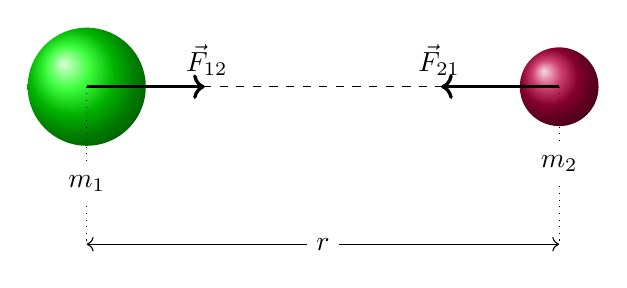
\begin{tikzpicture}
		\coordinate (A1) at (0,0);
		\coordinate (A2) at ($(A1)+(1.5cm,0)$);
		\coordinate (B1) at ($(A1)+(6cm,0)$);
		\coordinate (B2) at ($(B1)-(1.5cm,0)$);
		\shade[ball color=green] (A1) circle (0.75cm); 
		\shade[ball color=purple] (B1) circle (0.5cm);
		\draw[dashed] (A1) -- (B1);
		\draw[->,very thick] (A1)--(A2) node[near end,above right]{$\vec{F}_{12}$};
		\draw[->,very thick] (B1)--(B2) node[near end,above left]{$\vec{F}_{21}$};
		\coordinate (Ad) at ($(A1)-(0,2cm)$);
		\coordinate (Bd) at ($(B1)-(0,2cm)$);
		\draw[dotted] (A1) -- (Ad);
		\draw[dotted] (B1) -- (Bd);
		\draw[<->] (Ad) --(Bd);
		\node[below=1cm, fill=pagecol] at (A1) {$m_1$};
		\node[below=0.75cm, fill=pagecol] at (B1) {$m_2$};
		\node[fill=pagecol] at ($(Ad)!0.5!(Bd)$) {$r$};
	\end{tikzpicture}
\end{center}
Lực hấp dẫn giữa hai chất điểm bất kì tỉ lệ thuận với tích hai khối lượng của chúng và tỉ lệ nghịch với bình phương khoảng cách giữa chúng.
\begin{equation*}
	F_{\text {hd}} = G \dfrac {m_1 m_2 }{r^2},
\end{equation*}
trong đó:
\begin{itemize}
	\item $G$ là hằng số hấp dẫn, trong hệ SI có giá trị $G=\SI{6.67e-11}{\newton \meter ^2/\kilogram ^2}$;
	\item $m_1$, $m_2$ là khối lượng của hai vật;
	\item $r$ là khoảng cách giữa hai vật.
\end{itemize}

\subsubsection{Trọng lực }

Trọng lực là lực hấp dẫn của Trái Đất tác dụng vào vật gây ra cho chúng gia tốc rơi tự do. Trọng lực kí hiệu là $\vec P.$\\
Độ lớn của trọng lực:
\begin{equation*}
	P=F_{\text{hd}}=G \dfrac {mM}{(R+h)^2},
\end{equation*}
trong đó:
\begin{itemize}
	\item $m$ là khối lượng của vật ($\SI{}{\kilogram}$);
	\item $M$ là khối lượng Trái đất ($M \approx \SI{6e24}{\kilogram}$);
	\item $R$ là bán kính Trái đất ($R \approx \SI{6400e3}{\meter}$);
	\item $h$ là  độ cao của vật so với mặt đất ($\SI{}{\meter}$).
\end{itemize}

Gia tốc rơi tự do:
\begin{equation*}
	g=G \dfrac {M}{(R+h)^2}.
\end{equation*}
\begin{center}
	\includegraphics[scale=0.4]{../figs/VN10-PH-13-A-004-1-V2-01.jpg}
\end{center}
Ở gần Trái đất, trọng lực có phương thẳng đứng, có chiều từ trên xuống. \\
Công thức tính trọng lực: 
\begin{equation*}
	\vec P=m\vec g.
\end{equation*}

\subsubsection{Trọng lượng}
Khi vật đặt trong trọng trường và ở trạng thái cân bằng nhờ một dây treo hay giá đỡ, thì độ lớn của lực căng dây hoặc lực ép của vật lên giá đỡ gọi là trọng lượng của vật.  

\luuy{Không nên nhầm lẫn rằng trọng lượng là độ lớn của trọng lực. 
	
	Ví dụ, phi hành gia trên các trạm vũ trụ vẫn chịu tác dụng của trọng lực $P=mg$. Tuy nhiên nếu đặt một cái cân dưới chân phi hành gia thì cân chỉ số 0, vì trọng lực đã cân bằng với lực quán tính ly tâm (do trạm vũ trụ quay quanh Trái đất), nên phi hành gia không tạo được sức ép vào mặt cân. Ta nói phi hành gia ở trạng thái không trọng lượng (chứ không phải không trọng lực).}
\subsection{Lực căng dây}
\begin{minipage}[l]{0.5\textwidth}
	Khi kéo căng một sợi dây thì trong sợi dây xuất hiện lực căng chống lại xu hướng bị kéo dãn, gọi là lực căng dây. Lực căng dây kí hiệu là $\vec{T}$.

	Đối với dây không co giãn và khối lượng không đáng kể, độ lớn lực căng dây là như nhau tại mọi điểm trên dây. 
	
\end{minipage}
\begin{minipage}[r]{0.5\textwidth}
	\begin{center}
		\includegraphics[width=0.3\linewidth]{../figs/VN10-2023-PH-TP018-1}
		\captionof{figure}{Qủa cầu ở trạng thái cân bằng.}
	\end{center}
\end{minipage}
\section{Mục tiêu bài học - Ví dụ minh họa}
\begin{dang}{Ghi nhớ định luật vạn vật hấp dẫn. \\Nhận biết được đặc điểm của lực hấp dẫn}
	\viduii{1}{Lực hấp dẫn do một hòn đá ở trên mặt đất tác dụng vào Trái Đất thì có độ lớn
		\begin{mcq}(2)
			\item lớn hơn trọng lực của hòn đá.
			\item nhỏ hơn trọng lực của hòn đá.
			\item bằng trọng lực của hòn đá. 
			\item bằng 0.
		\end{mcq}
	}
	{	\begin{center}
			\textbf{Hướng dẫn giải}
		\end{center}
		
		Theo định luật III Newton: lực hấp dẫn do Trái Đất tác dụng lên hòn đá bằng lực hấp dẫn do hòn đá tác dụng lên Trái Đất.
		
		\textbf{Đáp án: C.}
	}
	\viduii{1}{Chọn phát biểu sai về lực hấp dẫn giữa hai vật?
		\begin{mcq}
			\item Lực hấp dẫn tăng 4 lần khi khoảng cách giảm đi một nửa .
			\item Lực hấp dẫn không đổi khi khối lượng một vật tăng gấp đôi còn khối lượng vật kia giảm còn một nửa.
			\item Rất hiếm khi lực hấp dẫn là lực đẩy.
			\item Hằng số hấp dẫn có giá trị như nhau ở cả trên mặt Trái Đất và trên Mặt Trăng.
		\end{mcq}
		
	}
	{	\begin{center}
			\textbf{Hướng dẫn giải}
		\end{center}
		
		Lực hấp dẫn luôn là lực hút.
		
		\textbf{Đáp án: C.}
	}
\end{dang}

\begin{dang}{Tính lực hấp dẫn và các đại lượng trong công thức của định luật vạn vật hấp dẫn}
	\viduii{3}{Cho biết khoảng cách giữa tâm Mặt Trăng và tâm Trái Đất là $\SI{38e7}{\meter}$; khối lượng Mặt Trăng và Trái Đất tương ứng là $\SI{7.37e22}{\kilogram}$ và $\SI{6e24}{\kilogram}$; hằng số hấp dẫn $G = \SI{6.67e-11}{\newton \meter ^2 / \kilogram ^2}$. Lực hấp dẫn giữa Trái Đất và Mặt Trăng có độ lớn là
		\begin{mcq}(2)
			\item $\SI{0.204e21}{\newton}$.
			\item $\SI{2.04e21}{\newton}$.
			\item $\SI{22e2}{\newton}$.
			\item $\SI{2e27}{\newton}$.
		\end{mcq}
	}
	{	\begin{center}
			\textbf{Hướng dẫn giải}
		\end{center}
		
		Áp dụng công thức lực hấp dẫn giữa Trái Đất và Mặt Trăng
		$$	F_{\text{hd}}=G\dfrac {m_1 m_2}{r^2} = \SI{0.204e21}{\newton}.$$
		
		\textbf{Đáp án: A.}
		
	}
	\viduii{3}{Hai quả cầu giống nhau được đặt sao cho hai tâm cách nhau khoảng $r$ thì lực hấp dẫn giữa chúng là $F$. Nếu thay một trong hai khối cầu trên bằng một khối cầu đồng chất khác nhưng có bán kính lớn gấp hai, vẫn giữ nguyên khoảng cách giữa hai tâm (hai khối cầu không chạm nhau) thì lực hấp dẫn giữa chúng lúc này là
		\begin{mcq}(4)
			\item $2F$.
			\item $4F$.
			\item $8F$.
			\item $16F$.
		\end{mcq}
		
	}
	{	\begin{center}
			\textbf{Hướng dẫn giải}
		\end{center}
		
		Gọi quả cầu 2 là quả cầu có bán kính tăng gấp đôi. Bán kính của quả cầu 2 lúc sau
		$$r_2 ' = 2 r_2.$$
		
		Nếu $D$ là khối lượng riêng của quả cầu thì khối lượng của quả cầu 2 lúc sau sẽ là 
		$$m_2 ' = D V_2 ' = D\cdot \dfrac{4}{3}\pi {r'}_2^3= D\cdot \dfrac {4}{3} \pi (2r_2) ^3 = 8 D\cdot \dfrac {4}{3}\pi r_2 ^3 = 8 D V_2 = 8 m_2. $$
		
		Lực hấp dẫn giữa hai quả cầu lúc sau
		$$F_\text{hd}' = G \dfrac{m_1 m_2 '}{r^2} = 8 G \dfrac {m_1 m_2}{r^2} = 8F.$$
		
		\textbf{Đáp án: C.}
	}
\end{dang}
\begin{dang}{Tính gia tốc rơi tự do và  trọng lượng vật trong các điều kiện khác nhau}
	\viduii{3}{Ở độ cao nào so với mặt đất thì gia tốc rơi tự do bằng một nửa gia tốc rơi tự do ở mặt đất? Cho bán kính Trái Đất là $R=\SI{6400}{\kilo \meter}$.
	}
	{	\begin{center}
			\textbf{Hướng dẫn giải}
		\end{center}
		
		Gia tốc rơi tự do ở mặt đất:
		$$g_0 = G \dfrac {M}{R^2}.$$
		
		Gia tốc rơi tự do ở độ cao $h$:
		$$g=G \dfrac {M}{(R+h)^2}.$$
		
		Gia tốc rơi tự do ở độ cao $h$ bằng một nửa gia tốc rơi tự do ở mặt đất, nên
		$$g=\dfrac{g_0}{2} \Rightarrow G \dfrac {M}{(R+h)^2} = G \dfrac {M}{2R^2} \Rightarrow (R+h)^2 = 2 R^2 \Rightarrow h=\SI{2650}{\kilo \meter}.$$
		
		Vậy ở độ cao $h=\SI{2650}{\kilo \meter}$ so với mặt đất thì gia tốc rơi tự do bằng một nửa so với gia tốc rơi tự do ở mặt đất.
		
	}
	\viduii{3}{Tính độ cao mà ở đó gia tốc rơi tự do là 9,6 m/s$^2$. Biết bán kính Trái Đất là 6400 km và gia tốc rơi tự do ở sát mặt đất là 9,8 m/s$^2$.
		
	}
	{	\begin{center}
			\textbf{Hướng dẫn giải}
		\end{center}
		
		Gia tốc rơi tự do ở độ cao $h$ 
		\begin{equation*}
			g = \dfrac{GM}{(R+h)^2} = \text{9,6}\ \text{m/s}^2.
		\end{equation*}
		Gia tốc rơi tự do ở sát mặt đất 
		\begin{equation*}
			g_0 = \dfrac{GM}{R^2} = \text{9,8}\ \text{m/s}^2.
		\end{equation*}
		Suy ra 
		\begin{equation*}
			\dfrac{g}{g_0}= \left(\dfrac{R}{R+h}\right)^2 =\text{0,98}\Rightarrow h = \dfrac{R(1- \sqrt{\text{0,98}})}{\sqrt {\text{0,98}}} = 65\ \text{km}.
		\end{equation*}
		
	}
\end{dang}
\begin{dang}{Mô tả được bằng ví dụ thực tiễn và biểu diễn được bằng hình vẽ: trọng lực, lực căng dây}
	\viduii{2}
	{Một bóng đèn có khối lượng $\SI{500}{\gram}$ được treo thẳng đứng vào trần nhà bằng một sợi dây và đang ở trạng thái cân bằng.
		\begin{enumerate}[label=\alph*)]
			\item Biểu diễn các lực tác dụng lên bóng đèn.
			\item Tính độ lớn của lực căng dây.
			\item Nếu dây treo chỉ chịu được một lực căng giới hạn $\SI{5.5}{\newton}$ thì nó có bị đứt không?
		\end{enumerate}
}
{\begin{center}
		\textbf{Hướng dẫn giải}
	\end{center}
\begin{enumerate}[label=\alph*)]
\begin{minipage}[l]{0.6\textwidth}
\item Các lực tác dụng lên bóng đèn gồm:
	\begin{itemize}
		\item Trọng lực phương thẳng đứng hướng xuống.
		\item Lực căng dây phương thẳng đứng hướng lên.
	\end{itemize}
\item Vì bóng đèn đang ở trạng thái cân bằng nên:
$$T=P=mg=\left(\SI{0.5}{\kilogram}\right)\cdot\left(\SI{9.8}{\meter/\second^2}\right)=\SI{4.9}{\newton}$$
\item Dây không bị đứt vì lực căng mà dây phải chịu là $\SI{4.9}{\newton}$ nhỏ hơn lực căng giới hạn.
\end{minipage}
\begin{minipage}{0.4\textwidth}
	\begin{center}
		\includegraphics[width=0.3\linewidth]{../figs/VN10-2023-PH-TP018-2}
	\end{center}
\end{minipage}
\end{enumerate}
}
\end{dang}
\begin{dang}{Tính các lực tác dụng lên vật \\khi vật cân bằng}
	\viduii{3}{Một vật có trọng lượng $P= 10$ N. được treo vào một vòng nhẫn O (coi là chất điểm). Vòng nhẫn được giữ yên bằng hai dây OA và OB. Biết dây OA nằm ngang và hợp với dây OB một góc $120^\circ.$ Tìm lực căng dây của hai dây OA và OB.
		
		\begin{center}
			\includegraphics[scale=0.5]{../figs/VN10-PH-11-L-008-4-V2-01.jpg}
		\end{center}
	}
	{	\begin{center}
			\textbf{Hướng dẫn giải}
		\end{center}
		\textbf{Cách 1: Áp dụng quy tắc tổng hợp lực.}
		\begin{center}
			\includegraphics[scale=0.8]{../figs/VN10-PH-11-L-008-4-V2-02.jpg}
		\end{center}
		Khi vật ở vị trí cân bằng thì các lực tác dụng lên vật gồm trọng lực $\vec{P}$, lực căng trên hai dây $\vec{T}_A$ và $\vec{T}_B$. Vòng nhẫn đứng yên nên các lực cân bằng nhau
		$$\vec{P}+\vec{T}_\textrm{A}+\vec{T}_\textrm{B}=\vec{0}.$$
		Gọi $\vec{Q}$ là hợp lực của $\vec{P}$ và $\vec{T}_A$
		$$\vec{P}+\vec{T}_\textrm{A}=\vec{Q}\quad\Rightarrow \quad\vec{T}_\textrm{B}+\vec{Q}=\vec{0}\quad\Rightarrow\quad \vec{T}_\textrm{B}=-\vec{Q}$$
		nghĩa là $\vec{Q}$ và $\vec{T}_B$ là hai vector trực đối. Do đó, $\alpha =\SI{	180}{\degree}-\SI{120}{\degree}=\SI{60}{\degree}.$
		
		Xét $\triangle$O$T_\text{A}$Q vuông tại $T_\text{A}$:
		
		$$\tan \alpha =\dfrac{P}{T_\text{A}}\Rightarrow T_\text{A}=\dfrac{P}{\tan \alpha}=\dfrac{10\sqrt{3}}{3}\,\text{N}.$$
		$$\sin \alpha =\dfrac{P}{Q}\Rightarrow Q=\dfrac{P}{\sin \alpha}=\dfrac{20\sqrt{3}}{3}\,\text{N}.$$
		Vì $|\vec{T}_\textrm{B}|=|\vec{Q}|$ nên $T_\textrm{B}= \dfrac{20\sqrt{3}}{3}\,\text{N}.$
		
		Vậy lực căng dây của hai dây OA và OB lần lượt bằng $\dfrac{10\sqrt{3}}{3}\,\text{N}, \dfrac{20\sqrt{3}}{3}\,\text{N}.$\\
		\textbf{Cách 2: Áp dụng quy tắc tam giác lực}\\
		Vòng nhẫn đứng yên nên các lực cân bằng nhau
		$$\vec{P}+\vec{T}_\textrm{A}+\vec{T}_\textrm{B}=\vec{0}.$$
		Do đó, $\left(\vec{P}, \overrightarrow{T_A}, \overrightarrow{T_B}\right)$ tạo thành tam giác khép kín
		\begin{center}
			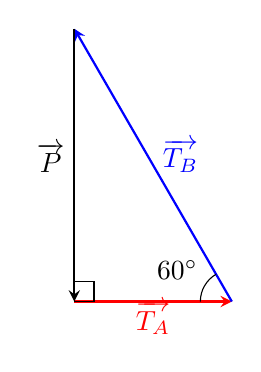
\begin{tikzpicture}
				\coordinate (O) at (2,0);
				\coordinate (A) at (0,0);
				\coordinate (B) at (0,3.464);
				\coordinate (O1) at (1,0);
				\coordinate (A1) at (1,1.73);
				\coordinate (B1) at (0,1.7);
				\draw[-stealth,thick, red] (A) -- (O);
				\draw[-stealth,thick, blue] (O) -- (B);
				\draw[-stealth,thick] (B) -- (A);
				\node[label={[red,below]90:$\overrightarrow{T_A}$}] at (O1){};	
				\node[label={[blue,right]90:$\overrightarrow{T_B}$}] at (A1){};	
				\node[label={[black,left]90:$\overrightarrow{P}$}] at (B1){};	
				\tkzMarkAngle[size=0.4,color=black](B,O,A);
				\tkzLabelAngle[color=black,pos=0.8](B,O,A){$\SI{60}{\degree}$}
				\tkzMarkRightAngle[draw=black,size=.25](B,A,O);
			\end{tikzpicture}
		\end{center}
		Từ tam giác vectơ ta xác định được 
		\begin{align*}
			\begin{cases}
				T_A=\dfrac{P}{\tan\SI{60}{\degree}}=\xsi{\dfrac{10\sqrt{3}}{3}}{\newton}\\
				T_B=\dfrac{P}{\sin\SI{60}{\degree}}=\xsi{\dfrac{20\sqrt{3}}{3}}{\newton}
			\end{cases}
		\end{align*}
		
	}
	\viduii{3}{Một đèn tín hiệu giao thông ở đại lộ có trọng 
		lượng 120 N được treo vào trung điểm của dây 
		AB làm dây thòng xuống $\text{0,5}$ m. Cho biết hai trụ treo dây cách nhau \SI{8}{\meter}, bỏ qua 
		trọng lượng của dây, tính lực căng mỗi sợi dây. 
		\begin{center}
			\includegraphics[scale=0.7]{../figs/VN10-PH-11-L-008-4-V2-03.jpg}
		\end{center}
	}
	{	\begin{center}
			\textbf{Hướng dẫn giải}
		\end{center}
		\textbf{Cách 1: Phân tích lực.}
		\begin{center}
			\includegraphics[scale=0.5]{../figs/VN10-PH-11-L-008-4-V2-04.jpg}
		\end{center}
		Đèn khi cân bằng chịu các lực tác dụng như hình vẽ, gồm trọng lực $\vec{P}$, hai lực căng dây $\vec{T}_1$ và $\vec{T}_2$
		\begin{align*}
			\vec{P}+\vec{T}_1+\vec{T}_2=0
		\end{align*}
		
		Gọi $\vec T$ là hợp lực của hai dây cáp:
		$$\vec{T}=\vec{T}_1+\vec{T}_2\quad\Rightarrow\quad \vec{P}+\vec{T}=0$$
		nghĩa là $T=P=mg=\SI{120}{\newton}$.
		
		Do tính đối xứng, hai lực căng dây phải có độ lớn bằng nhau $T_1=T_2$. Từ hình vẽ 
		\begin{align*}
			T=2T_1\cos \alpha\quad\Rightarrow\quad T_1=\dfrac{T}{2\cos\alpha}
		\end{align*}
		trong đó góc $\alpha$ được xác định từ tam giác vuông bên phải trên hình
		\begin{align*}
			\tan\alpha=\dfrac{\SI{4}{\meter}}{\SI{0.5}{\meter}}=8\quad\Rightarrow\quad \alpha\approx\SI{82.875}{\degree}. 
		\end{align*}
		Từ đó ta tính được lực căng dây
		\begin{align*}
			T_1=T_2=\dfrac{T}{2\cos\alpha}\approx \SI{484}{\newton}.
		\end{align*}		
	\textbf{Cách 2: Dùng tam giác lực}\\
	Đèn cân bằng nên
	\begin{align*}
		\vec{P}+\vec{T}_1+\vec{T}_2=\overrightarrow{0}
	\end{align*}
Do tính đối xứng, hai lực căng dây phải có độ lớn bằng nhau $T_1=T_2$.\\
Ba vectơ lực $\vec{P}, \overrightarrow{T_1}, \overrightarrow{T_2}$ tạo thành tam giác vectơ khép kín
	\begin{center}
	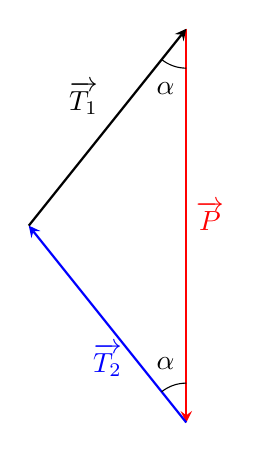
\begin{tikzpicture}
		\coordinate (O) at (0,0);
		\coordinate (A) at (0,-5);
		\coordinate (B) at (-2,-2.5);
		\coordinate (O1) at (0,-2.5);
		\coordinate (A1) at (-1,-4);
		\coordinate (B1) at (-1,-1);
		\draw[-stealth,thick, red] (O) -- (A);
		\draw[-stealth,thick, blue] (A) -- (B);
		\draw[-stealth,thick] (B) -- (O);
		\node[label={[red,right]90:$\overrightarrow{P}$}] at (O1){};	
		\node[label={[blue,below]90:$\overrightarrow{T_2}$}] at (A1){};	
		\node[label={[black,left]90:$\overrightarrow{T_1}$}] at (B1){};	
		\tkzMarkAngle[size=0.5,color=black](O,A,B);
		\tkzLabelAngle[color=black,pos=0.8](O,A,B){$\alpha$};
		\tkzMarkAngle[size=0.5,color=black](B,O,A);
		\tkzLabelAngle[color=black,pos=0.8](B,O,A){$\alpha$}
	\end{tikzpicture}
\end{center}
Áp dụng định lý hàm sin:
\begin{align*}
	\dfrac{T_1}{\sin\alpha}&=\dfrac{P}{\sin\left(\SI{180}{\degree}-2\alpha\right)}\Leftrightarrow \dfrac{T_1}{\sin\alpha}=\dfrac{P}{\sin\left[2\cdot\left(\SI{90}{\degree}-\alpha\right)\right]}\\
	\Rightarrow \dfrac{T_1}{\sin\alpha}&=\dfrac{P}{2\sin\left(\SI{90}{\degree}-\alpha\right)\cos\left(\SI{90}{\degree}-\alpha\right)}=\dfrac{P}{2\cos\alpha\sin\alpha}\\
	\Rightarrow T_1&=\dfrac{P}{2\cos\alpha}\approx\SI{484}{\newton}
\end{align*}
	}
	
	
\end{dang}
%\let\lesson\undefined
\newcommand{\lesson}{\phantomlesson{Bài 12: Một số lực trong thực tiễn}}
\chapter[Lực ma sát]{Lực ma sát}
\setcounter{section}{0}
\section{Lý thuyết}
\subsection{Lực ma sát nghỉ}
\subsubsection{Định nghĩa}
Lực ma sát nghỉ xuất hiện ở mặt tiếp xúc khi một vật nằm yên trên bề mặt vật khác và có xu hướng chuyển động dưới tác dụng của ngoại lực.
\begin{center}
	\includegraphics[width=0.4\linewidth]{../figs/VN10-2023-PH-TP019-1}
	\captionof{figure}{Thùng gỗ bất động khi bị người đẩy.}
\end{center}
\subsubsection{Đặc điểm}
\begin{itemize} 
	\item Điểm đặt: trên vật và ngay tại vị trí tiếp xúc của hai bề mặt, 
	\item Phương: tiếp tuyến với bề mặt tiếp xúc,
	\item Chiều: ngược chiều xu hướng chuyển động tương đối của hai bề mặt tiếp xúc,
	\item Độ lớn: bằng độ lớn của lực tác dụng gây ra xu hướng chuyển động.
\end{itemize}
\luuy{Điều kiện để vật bắt đầu trượt 
$$F_{ms}\ge F_{msn\ \text{max}}=\mu_N\cdot N$$
trong đó:
\begin{itemize}
	\item $F_{msn\ \text{max}}$: lực ma sát nghỉ cực đại;
	\item $\mu_N$: hệ số ma sát nghỉ;
	\item $N$: áp lực do vật tác dụng lên bề mặt tiếp xúc.
\end{itemize}
Lực ma sát nghỉ cực đại lớn hơn ma sát trượt.
}
\subsection{Lực ma sát trượt}
\subsubsection{Định nghĩa}
Lực ma sát trượt xuất hiện ở mặt tiếp xúc khi một vật trượt trên một bề mặt và cản trở lại chuyển động trượt của vật đó.
\begin{center}
	\includegraphics[scale=0.35]{../figs/VN10-PH-15-L-012-1-V2-01.JPG}
\end{center}
\subsubsection{Đặc điểm}
\begin{itemize}
	\item Điểm đặt: trên vật và ngay tại vị trí tiếp xúc của hai bề mặt,
	\item Phương: tiếp tuyến với mặt tiếp xúc giữa 2 vật trượt,
	\item Chiều: ngược chiều với vận tốc tương đối của vật ấy đối với vật kia,
	\item Độ lớn:
	\begin{itemize}
		\item không phụ thuộc vào diện tích tiếp xúc và tốc độ của vật.
		\item tỉ lệ với độ lớn của áp lực.
		\item phụ thuộc vào vật liệu và tình trạng của hai mặt tiếp xúc.
	\end{itemize}
	\item Biểu thức 
	\begin{equation*}
		F_{\text{mst}} = \mu_{\text{t}} \cdot N,
	\end{equation*}
	trong đó:
	
	+ $\mu_{\text{t}}$ là hệ số ma sát trượt, nó phụ thuộc vào bản chất của hai mặt tiếp xúc và các điều kiện trên bề mặt (không có đơn vị),
	
	+ $N$ là áp lực của vật lên mặt tiếp xúc.
\end{itemize}
\subsubsection{Vai trò}
\begin{itemize}
	\item Ma sát trượt có ích trong việc mài dũa, thắng xe, \dots
	\item Ma sát trượt có hại trong các ổ trục trượt, mài mòn xilanh, pittông xe, \dots Để giảm ma sát trượt, người ta bôi trơn các chi tiết bằng dầu mỡ công nghiệp.
\end{itemize}
\subsection{Lực ma sát lăn}
\begin{itemize}
	\item Lực ma sát lăn xuất hiện ở mặt tiếp xúc khi một vật lăn trên một bề mặt và cản trở lại chuyển động lăn của vật đó.
	\item Lực ma sát lăn có các đặc điểm giống như lực ma sát trượt nhưng hệ số ma sát lăn nhỏ hơn rất nhiều lần (hàng chục lần) hệ số ma sát trượt.
	\item Trong trường hợp lực ma sát trượt có hại, cần phải giảm thì người ta dùng con lăn hay ổ bi đặt xen vào giữa hai mặt tiếp xúc để giảm tổn hại vì ma sát.
\end{itemize}
\begin{center}
	\includegraphics[scale=0.25]{../figs/VN10-PH-15-L-012-1-V2-02.JPG}
\end{center}

\subsubsection{Vai trò}
\begin{itemize}
	\item Giúp ta cầm nắm được các vật, giữ vật ở yên tại vị trí đã định, dây cua roa truyền được chuyển động giữa các bánh xe, băng chuyền vận chuyển được người hoặc vật từ nơi này đến nơi khác...
	\item Đóng vai trò lực phát động, giúp sinh vật, xe cộ di chuyển được.
	\begin{center}
		\includegraphics[scale=0.35]{../figs/VN10-PH-15-L-012-1-V2-03.JPG}
		\captionof{figure}{Lực ma sát do mặt đất tác dụng lên chân người khi đi sẽ làm cho người có thể tiến về phía trước.}
	\end{center}
	\item Trong những trường hợp ma sát có lợi, người ta tìm cách tăng tính nhám của các mặt tiếp xúc và tăng áp lực lên mặt tiếp xúc, chẳng hạn thêm các rãnh trên đế giày, bánh xe để tăng ma sát.
\end{itemize}

\section{Mục tiêu bài học - Ví dụ minh họa}
\begin{dang}{Ghi nhớ khái niệm các loại lực ma sát}
	\viduii{1}{Hệ số ma sát trượt
		\begin{mcq}
			\item tỉ lệ thuận với lực ma sát trượt và tỉ lệ nghịch với áp lực. 
			\item phụ thuộc diện tích tiếp xúc và tốc độ của vật.
			\item phụ thuộc vào vật liệu và tình trạng của mặt tiếp xúc. 
			\item phụ thuộc vào áp lực.
		\end{mcq}
	}
	{	\begin{center}
			\textbf{Hướng dẫn giải}
		\end{center}
		
		Hệ số ma sát trượt phụ thuộc vào vật liệu và tình trạng của mặt tiếp xúc   
		
		\textbf{Đáp án: C}.
	}
	\viduii{1}{Chiều của lực ma sát nghỉ
		\begin{mcq}
			\item  Ngược chiều với vận tốc của vật.
			\item  Ngược chiều với gia tốc của vật.
			\item  Ngược chiều với thành phần ngoại lực song song với mặt tiếp xúc.
			\item  Vuông góc với mặt tiếp xúc.
		\end{mcq}
	}
	{	\begin{center}
			\textbf{Hướng dẫn giải}
		\end{center}
		
		Chiều của lực ma sát nghỉ ngược chiều với thành phần ngoại lực song song với mặt tiếp xúc.
		
		\textbf{Đáp án: C}.
	}
	\viduii{1}{Phát biểu nào sau đây là đúng khi nói về ma sát
		\begin{mcq}
			\item Lực ma sát lăn cản trở chuyển động của vật này trượt trên vật khác.
			\item Khi vật chuyển động chậm dần, lực ma sát nhỏ hơn lực đẩy.
			\item Lực ma sát lăn nhỏ hơn lực ma sát trượt.
			\item Khi vật chuyển động nhanh dần, lực ma sát lớn hơn lực đẩy.
		\end{mcq}
	}
	{	\begin{center}
			\textbf{Hướng dẫn giải}
		\end{center}
		
		A - sai vì: lực ma sát lăn cản trở chuyển động của vật này lăn trên vật khác
		
		B - sai vì: khi vật chuyển động chậm dần, lực ma sát lớn hơn lực đẩy
		
		C - đúng
		
		D - sai vì: khi vật chuyển động nhanh dần, lực ma sát nhỏ hơn lực đẩy
		
		\textbf{Đáp án: C}.
	}
\end{dang}
\begin{dang}{Tính độ lớn lực ma sát và các đại lượng\\ trong công thức lực ma sát trượt}
	\viduii{2}{Một ô tô khối lượng 1,5 tấn chuyển động thẳng đều trên đường. Hệ số ma sát lăn giữa bánh xe và mặt đường là 0,08. Tính lực làm cản trở chuyển động của xe trên mặt đường (bỏ qua lực cản không khí).
	}
	{	\begin{center}
			\textbf{Hướng dẫn giải}
		\end{center}
		\manatip{Trong trường hợp xe chuyển động do lực đẩy của động cơ, ta xem như lực này có phương song song với mặt đất.}
		
		Lực đẩy song song với mặt ngang, nên phản lực có độ lớn bằng với trọng lực. Lực làm cản trở chuyển động của xe trên mặt đường là lực ma sát
		\begin{equation*}
			F_{\text{ms}} =\mu N = \mu  mg =\SI{0.08}{}\cdot(\SI{1.5e3}{\kilogram})\cdot\SI{9.81}{\meter/\second^{2}}\approx \SI{1177}{N}.
		\end{equation*}
		
		
	}
	\viduii{2}{Một toa tàu có khối lượng 80 tấn chuyển động thẳng đều dưới tác dụng của lực kéo $F = 6\cdot 10^4\ \text{N}$. Xác định lực ma sát và hệ số ma sát giữa toa tàu với mặt đường
	}
	{	\begin{center}
			\textbf{Hướng dẫn giải}
		\end{center}
		
		Tàu chuyển động thẳng đều nên lực ma sát cân bằng với lực kéo của toa tàu
		\begin{equation*}
			F_{\text{ms}} = F_{\text{k}} = \mu mg.
		\end{equation*}
		Suy ra hệ số ma sát
		\begin{equation*}
			\mu = \dfrac{F_{\text{k}}}{mg} = \text{0,075}.
		\end{equation*} 
	}
	\viduii{2}{Một ô tô nặng 1,5 tấn chuyển động trên đường nằm ngang chịu tác dụng của lực phát động $\SI{3300}{\newton}$. Cho xe chuyển động với vận tốc đầu $\SI{10}{\meter/\second}$. Sau khi đi $\SI{75}{\meter}$ thì ô tô đạt vận tốc $\SI{72}{\kilo\meter/\hour}$. Lực ma sát giữa xe và mặt đường có độ lớn là bao nhiêu?
	}
	{	\begin{center}
			\textbf{Hướng dẫn giải}
		\end{center}
		$$\SI{72}{\kilo\meter/\hour}=\SI{2}{\meter/\second}$$
		Gia tốc của ô tô 
		\begin{equation*}
			v^2-v^2_0 = 2as \Rightarrow a = \dfrac{v^2-v^2_0}{2s} = \SI{2}{m/s^2}.
		\end{equation*}
		Áp dụng định luật II Newton và chiếu lên chiều chuyển động của vật
		\begin{equation*}
			-F_{\text{ms}}+F = ma \Rightarrow F_{\text{ms}} = F-ma = \SI{300}{N}.
		\end{equation*}
		
	}
\end{dang}
\begin{dang}{Giải bài toán vật chuyển động trên mặt phẳng ngang có ma sát}
	\viduii{3}{Một ô tô khối lượng 1 tấn, chuyển động trên mặt đường nằm ngang. Hệ số ma sát lăn giữa xe và mặt đường là 0,1. Tính lực kéo của động cơ ô tô trong mỗi trường hợp sau
		
		a) Ô tô chuyển động thẳng đều.
		
		b) Ô tô chuyển động nhanh dần đều với gia tốc $a = \SI{2}{m/s}^2$, lấy $g=\SI{10}{m/s^2}$.
	}
	{	\begin{center}
			\textbf{Hướng dẫn giải}
		\end{center}
		\begin{center}
			\includegraphics[scale=0.6]{../figs/VN10-PH-15-A-005-3-V2-03.JPG}
		\end{center} 
		Áp dụng định luật II Newton
		\begin{equation*}
			\vec{N}+\vec{P} + \vec{F}_{\text{ms}} + \vec{F} = m\vec{a}.
		\end{equation*}
		Chiếu lên O$y$:
		\begin{equation*}
			N=P = mg.
		\end{equation*}
		Chiếu lên O$x$:
		\begin{equation*}
			F-F_{\text{ms}} = ma \Rightarrow F = ma + F_{\text{ms}}
		\end{equation*}
		a) Khi ô tô chuyển động thẳng đều thì $a=0$ nên lực kéo của ô tô đúng bằng lực ma sát
		\begin{equation*}
			F=F_{\text{ms}} = \mu mg = \SI{1000}{N}.
		\end{equation*}
		b) Khi ô tô chuyển động nhanh dần đều với gia tốc $a = \SI{2}{m/s^2}$ 
		\begin{equation*}
			F= ma + F_{\text{ms}} = ma + \mu mg = m(a+ \mu g) = \SI{3000}{N}.
		\end{equation*}
		
	}
	
	\viduii{3}{Một xe lăn, khi được đẩy bằng lực $F = \SI{20}{N}$ nằm ngang thì xe chuyển động thẳng đều. Khi chất lên xe một kiện hàng khối lượng $\SI{20}{kg}$ thì phải chịu tác dụng lực $F = \SI{60}{N}$ nằm ngang xe mới chuyển động thẳng đều. Tính hệ số ma sát giữa xe và mặt dường.
	}
	{	\begin{center}
			\textbf{Hướng dẫn giải}
		\end{center}
		
		Chọn chiều dương là chiều chuyển động của xe.
		
		Khi chưa chất kiện hàng lên xe, xe chuyển động thằng đều nên:
		
		$$\vec P + \vec N + \vec F_\text{ms} + \vec F = \vec 0 \Rightarrow - F_\text{ms} + F =0 \Rightarrow F =F_\text{ms} = \mu mg\ (1).$$
		
		Khi đã chất kiện hàng lên xe, xe chuyển động thẳng đều nên:	
		
		$$\vec P' + \vec N' + \vec F'_\text{ms} + \vec F' = \vec 0 \Rightarrow - F'_\text{ms} + F' =0 \Rightarrow F' =F'_\text{ms} = \mu (m+m_\text{h})g\ (2).$$
		
		Từ (1) và (2) suy ra: 
		
		$$F' - F = \mu g m_\text{h} \Rightarrow \mu =\dfrac{F'-F}{gm_\text{h}} = \SI{0,2}{}.$$
		
		
	}
	
\end{dang}
%\let\lesson\undefined
\newcommand{\lesson}{\phantomlesson{Bài 12: Một số lực trong thực tiễn}}
\chapter[Lực cản và lực nâng của chất lưu]{Lực cản và lực nâng của chất lưu}
\setcounter{section}{0}
\section{Lý thuyết}
\subsection{Lực đẩy Archimedes}
Mọi vật chìm trong chất lưu (chất lỏng, không khí, \dots) đều chịu tác dụng của lực nâng. Lực nâng này được gọi là lực đẩy Archimedes và có đặc điểm như sau:
\begin{center}
	\includegraphics[width=0.25\linewidth]{../figs/VN10-2023-PH-TP020-1}
	\captionof{figure}{Trọng lực và lực đẩy Archimedes tác dụng lên vật.}
\end{center}
\begin{itemize}
	\item Điểm đặt: trọng tâm của phần chất lưu bị vật chiếm chỗ;
	\item Phương: thẳng đứng;
	\item Chiều: từ dưới lên trên;
	\item Độ lớn: bằng trọng lượng phần chất lưu bị vật chiếm chỗ
	$$F_A=\rho \cdot g \cdot V$$
	trong đó:
	\begin{itemize}
		\item $F_A$: độ lớn lực đẩy Archimedes tác dụng lên phần vật chìm $\left(\si{\newton}\right)$;
		\item $\rho$: khối lượng riêng của chất lưu $\si{\kilogram/\meter^3}$;
		\item $g$: gia tốc trọng trường $\si{\meter/\second^2}$;
		\item $V$: thể tích phần chất lưu bị vật chiếm chỗ $\si{\meter^3}$.
	\end{itemize}
\end{itemize}
\subsection{Áp suất chất lỏng}
\subsubsection{Định nghĩa áp suất}
Áp suất là đại lượng được xác định bằng độ lớn áp lực $F$ trên một đơn vị diện tích $S$ của mặt bị ép
$$p=\dfrac{F}{S}$$
Trong hệ SI, đơn vị của áp suất là $\si{\pascal}$ $\left(\SI{1}{\pascal}=\SI{1}{\newton/\meter^2}\right)$.\\
Trong chất lỏng luôn tồn tại áp suất do trọng lượng của chất lỏng tạo ra.
\subsubsection{Khối lượng riêng}
Khối lượng riêng của một chất là đại lượng được xác định bằng khối lượng $m$ của vật tạo thành từ chất đó trên một đơn vị thể tích $V$ của vật
$$\rho=\dfrac{m}{V}$$
Trong hệ SI, đơn vị của khối lượng riêng là $\si{\kilogram/\meter^3}$.
\subsubsection{Độ chênh lệch áp suất giữa hai điểm trong lòng chất lỏng}
Xét hai điểm $A$ và $B$ cách nhau một đoạn $\Delta h$ theo phương thẳng đứng trong chậu chứa một chất lỏng xác định. Độ chênh lệch áp suất giữa hai điểm $A$ và $B$
$$\Delta p=\rho \cdot g\cdot \Delta h$$
\subsection{Lực cản của chất lưu}
Khi chuyển động trong không khí, trong nước hoặc trong chất lỏng nói chung (gọi chung là chất lưu), vật đều chịu tác dụng của lực cản.
\begin{center}
	\includegraphics[width=0.4\linewidth]{../figs/VN10-2023-PH-TP020-2}
	\captionof{figure}{Đồ thị tốc độ theo thời gian của vật rơi trong chất lưu khi có lực cản.}
\end{center}
Chuyển động của vật trong chất lưu được chia thành 3 giai đoạn:
\begin{itemize}
	\item Nhanh dần đều từ lúc bắt đầu rơi trong một thời gian ngắn.
	\item Nhanh dần không đều trong một khoảng thời gian tiếp theo. Lúc này lực cản bắt đầu có độ lớn đáng kể và tăng dần.
	\item Chuyển động đều với tốc độ giới hạn không đổi. Khi đó, tổng hợp lực tác dụng lên vật rơi bị triệt tiêu.
\end{itemize}
\luuy{Sau khi vật chuyển động đều, nếu có thêm tác nhân làm tăng lực cản của chất lưu (ví dụ như người nhảy dù bung dù ra như trong Hình \ref{fig:20.3}), thì vật sẽ chuyển động chậm dần. Tốc độ rơi của vật giảm dần, lực cản cũng giảm đến khi tổng lực tác dụng lên vật lại bị triệt tiêu và vật trở lại trạng thái chuyển động đều.
\begin{center}
	\includegraphics[width=0.4\linewidth]{../figs/VN10-2023-PH-TP020-3}
	\captionof{figure}{a) chưa bung dù; b) chuyển động ổn định khi chưa bung dù; c) vừa bung dù; d) chuyển động ổn định.}
	\label{fig:20.3}
\end{center}
}
Lực cản của chất lưu được biểu diễn bởi một lực đặt tại trọng tâm vật, cùng phương và ngược chiều với chiều chuyển động của vật trong chất lưu. Lực cản này phụ thuộc vào hình dạng và tốc độ của vật.
\section{Mục tiêu bài học - Ví dụ minh hoạ}
\begin{dang}{Thành lập và vận dụng được phương trình $\Delta p=\rho\cdot g\cdot\Delta h$ trong một số trường hợp đơn giản}
	\viduii{3}
	{Em hãy xây dựng biểu thức xác định độ chênh lệch áp suất giữa hai điểm có độ sâu khác nhau trong lòng chất lỏng.
}
{\begin{center}
		\textbf{Hướng dẫn giải}
	\end{center}
Xét hai điểm $A$ và $B$ cách nhau một đoạn $\Delta h$ theo phương thẳng đứng trong chậu chứa một chất lỏng xác định. Giả định hai điểm $A$ và $B$ nằm trên hai mặt đáy của một bình chứa hình hộp chữ nhật tiết diện $S$, độ cao $\Delta h$ như Hình \ref{fig:20.4}.
\begin{center}
	\includegraphics[width=0.3\linewidth]{../figs/VN10-2023-PH-TP020-4}
	\captionof{figure}{Hai điểm $A$ và $B$ trong lòng chất lỏng có thể được giả định thành hai điểm $A$ và $B$ nằm trên hai mặt đáy của một bình chứa hình hộp chữ nhật.}
	\label{fig:20.4}
\end{center}
Độ chênh lệch áp suất $\Delta p$ giữa hai đáy là do trọng lượng $mg$ của phần chất lỏng hình trụ có khối lượng $m$ gây ra trên một đơn vị diện tích. Theo định nghĩa áp suất, ta có
\begin{equation}
	\Delta p =\dfrac{mg}{S}
	\label{eq:20.1}
\end{equation}
Khối lượng của phần chất lỏng này được suy ra từ khối lượng riêng và thể tích của nó
$$m=\rho\cdot V=\rho \cdot S\cdot\Delta h$$
Thay vào biểu thức (\ref{eq:20.1}), ta có:
$$\Delta p=\rho\cdot g\cdot \Delta h$$
}
\viduii{3}
{Kỉ lục thế giới về lặn tự do (không có bình dưỡng khí) được thực hiện bởi một nữ thợ lặn người Slovenia khi cô lặn xuống biển tới độ sâu $\SI{114}{\meter}$. Hãy tính độ chênh lệch áp suất tại vị trí này so với mặt thoáng của nước biển. Lấy giá trị trung bình khối lượng riêng của nước biển là $\SI{1025}{\kilogram/\meter^3}$ và $g=\SI{9.8}{\meter/\second^2}$.
}
{\begin{center}
		\textbf{Hướng dẫn giải}
	\end{center}
Độ chênh lệch áp suất tại vị trí có độ sâu $\SI{114}{\meter}$ so với mặt thoáng của nước biển:
$$\Delta p=\rho g\Delta h=\left(\SI{1025}{\kilogram/\meter^3}\right)\cdot\left(\SI{9.8}{\meter/\second^2}\right)\cdot\left(\SI{114}{\meter}\right)\approx\SI{11.45E5}{\pascal}$$
}
\end{dang}
\begin{dang}{ Mô tả được bằng ví dụ thực tiễn và biểu diễn được bằng hình vẽ: lực cản, lực nâng của chất lưu}
	\viduii{2}
	{Hãy vẽ lực cản của không khí hoặc nước tác dụng lên các vật trong các trường hợp được mô tả trong Hình \ref{fig:20.5}
		\begin{center}
			\includegraphics[width=0.6\linewidth]{../figs/VN10-2023-PH-TP020-5}
			\captionof{figure}{a) Con chim ruồi đang bay theo phương xiên hướng lên trên; b) Tàu ngầm đang di chuyển lên trên mặt nước theo phương thẳng đứng; c) Máy bay đang bay theo phương ngang.}
			\label{fig:20.5}
		\end{center}
}
{\begin{center}
		\textbf{Hướng dẫn giải}
	\end{center}
Lực cản tác dụng lên vật được biểu diễn như hình vẽ:
\begin{center}
	\includegraphics[width=0.6\linewidth]{../figs/VN10-2023-PH-TP020-6}
\end{center}
}
\viduii{2}
{Một con cá hề đang bơi trong nước chịu tác dụng của lực cản $F=0,65v$ ($v$ là tốc độ tức thời tính theo đơn vị $\si{\meter/\second}$). Hãy tính lực tối thiểu để con cá đạt tốc độ $\SI{6}{\meter/\second}$, giả sử con cá bơi theo phương ngang.
	\begin{center}
		\includegraphics[width=0.2\linewidth]{../figs/VN10-2023-PH-TP020-7}
		\captionof{figure}{Cá hề}
	\end{center}
}
{\begin{center}
		\textbf{Hướng dẫn giải}
	\end{center}
Lực tối thiểu để con cá đạt được tốc độ $\SI{6}{\meter/\second}$ là 
$$F_\text{min}=F=0,65v=0,65\cdot6=\SI{3.9}{\newton}$$
}
\end{dang}
\begin{dang}{Giải thích được lực nâng tác dụng lên một vật ở trong trong nước (hoặc trong không khí)}
	\viduii{3}
	{\begin{minipage}[l]{0.6\textwidth}
			Một vật được móc vào lực kế như Hình \ref{fig:20.8}. Khi để ở ngoài không khí, lực kế chỉ $\SI{5}{\newton}$. Khi nhúng chìm hoàn toàn vật trong nước thì thấy lực kế chỉ $\SI{3.2}{\newton}$.
			\begin{enumerate}[label=\alph*)]
				\item Mô tả và biểu diễn các lực tác dụng lên vật.
				\item Tính lực đẩy Archimedes tác dụng lên vật.
			\end{enumerate}
		\end{minipage}
		\begin{minipage}{0.4\textwidth}
			\begin{center}
				\includegraphics[width=0.25\linewidth]{../figs/VN10-2023-PH-TP020-8}
				\captionof{figure}{}
				\label{fig:20.8}
			\end{center}
		\end{minipage}
}
{\begin{center}
		\textbf{Hướng dẫn giải}
	\end{center}
\begin{enumerate}[label=\alph*)]
	\begin{minipage}[l]{0.5\textwidth}
		\item Khi nhúng chìm hoàn toàn vật trong nước, các lực tác dụng lên vật gồm:
		\begin{itemize}
			\item Trọng lực $\vec{P}$;
			\item Lực đẩy Archimedes $\overrightarrow{F_A}$;
			\item Lực kéo của lực kế $\vec{F}$.
		\end{itemize}
	\item Khi để lực kế ngoài không khí, số chỉ của lực kế là độ lớn trọng lực của vật
	$P=\SI{5}{\newton}$.\\
	Vật nằm cân bằng trong nước:
	$$\overrightarrow{P}+\overrightarrow{F_A}+\overrightarrow{F}=\vec{0}$$
	Chiếu lên hướng của $\overrightarrow{F}$, ta có:
	$$-P+F_A+F=0\Rightarrow F_A=P-F=\SI{1.8}{\newton}$$
	\end{minipage}
	\begin{minipage}{0.5\textwidth}
		\begin{center}
			\includegraphics[width=0.3\linewidth]{../figs/VN10-2023-PH-TP020-9}
		\end{center}
	\end{minipage}

\end{enumerate}
}
\viduii{3}
{Một khối gỗ hình hộp chữ nhật có tiết diện $S=\SI{40}{\centi\meter^2}$ cao $h=\SI{10}{\centi\meter}$. Khối gỗ có khối lượng $m=\SI{160}{\gram}$. Thả khối gỗ vào nước, khối gỗ nổi lơ lửng trên mặt nước như hình \ref{fig:20.10}. Khối lượng riêng của nước là $\rho=\SI{1000}{\kilogram/\meter^3}$. Tìm chiều cao của phần gỗ nổi trên mặt nước.
	\begin{center}
		\includegraphics[width=0.2\linewidth]{../figs/VN10-2023-PH-TP020-10}
		\captionof{figure}{}
		\label{fig:20.10}
	\end{center}
}
{\begin{center}
		\textbf{Hướng dẫn giải}
	\end{center}
Gọi $x$ là chiều cao phần khối gỗ nhô ra khỏi mặt nước, khi đó chiều cao phần khối gỗ chìm trong nước là $\left(h-x\right)$.\\
Thể tích phần gỗ chìm trong nước
$$V=S\left(h-x\right)$$
Khi khối gỗ cân bằng trong nước thì trọng lực của khối gỗ cân bằng với lực đẩy Archimedes
$$P=F_A\Leftrightarrow mg=\rho gV=\rho g S\left(h-x\right)$$
$$\Rightarrow x=h-\dfrac{m}{\rho S}=\left(\SI{0.1}{\meter}\right)-\dfrac{\left(\SI{0.16}{\kilogram}\right)}{\left(\SI{1000}{\kilogram/\meter^3}\right)\cdot\left(\SI{40E{-4}}{\meter^2}\right)}=\SI{0.06}{\meter}=\SI{6}{\centi\meter}.$$
}
\end{dang}
%\input{../dataSG/VN10-2023-PH-TP021}
\setcounter{mychap}{4}
\mychap{Moment lực. Điều kiện cân bằng.}
%\let\lesson\undefined
\newcommand{\lesson}{\phantomlesson{Bài 13: Tổng hợp lực song song cùng chiều}}
\chapter[Tổng hợp hai lực song song cùng chiều]{Tổng hợp hai lực song song cùng chiều}
\setcounter{section}{0}
\section{Lý thuyết}
Lực tổng hợp của hai lực song song cùng chiều là một lực:
\begin{itemize}
	\item Song song, cùng chiều với các lực thành phần.
	\item Có độ lớn bằng tổng độ lớn của các lực thành phần:
	$$F_t=F_1+F_2$$
	\item Có giá nằm trong mặt phẳng của hai lực thành phần, chia khoảng cách giữa hai giá của hai lực song song thành những đoạn tỉ lệ nghịch với độ lớn của hai lực ấy
	$$\dfrac{F_1}{F_2}=\dfrac{d_2}{d_1}.$$
\end{itemize}
\begin{center}
	\includegraphics[width=0.35\linewidth]{../figs/VN10-2023-PH-TP022-2}
\end{center}
\section{Mục tiêu bài học - Ví dụ minh hoạ}
\begin{dang}{Xác định lực tổng hợp của hai lực song song cùng chiều}
	\viduii{3}
	{Một người đang gánh lúa như hình \ref{fig:22.2}. Hỏi vai người phải đặt ở vị trí nào trên đòn gánh để đòn gánh có thể nằm ngang cân bằng trong quá trình di chuyển? Biết khối lượng hai bó lúa lần lượt là $m_1=\SI{7}{\kilogram}$, $m_2=\SI{5}{\kilogram}$ và chiều dài đòn gánh là $\SI{1.5}{\meter}$. Xem như điểm treo hai bó lúa sát hai đầu đòn gánh và bỏ qua khối lượng đòn gánh.
	\begin{center}
		\includegraphics[width=0.3\linewidth]{../figs/VN10-2023-PH-TP022-1}
		\captionof{figure}{Người nông dân gánh lúa ở hai đầu đòn gánh.}
		\label{fig:22.2}
	\end{center}
}
{\begin{center}
		\textbf{Hướng dẫn giải}
	\end{center}
Áp dụng quy tắc tổng hợp lực song song cùng chiều, để đòn gánh cân bằng thì
\begin{equation}
	\label{eq:22.1}
	\dfrac{d_2}{d_1}=\dfrac{F_1}{F_2}=\dfrac{m_1g}{m_2g}=\dfrac{7}{5}
\end{equation}
mà
\begin{equation}
	\label{eq:22.2}
	d_1+d_2=\SI{1.5}{\meter}
\end{equation}
Từ (\ref{eq:22.1}) và (\ref{eq:22.2}), ta thu được:
\begin{align*}
	\begin{cases}
		d_1=\SI{0.625}{\meter}\\
		d_2=\SI{0.875}{\meter}.
	\end{cases}
\end{align*}
}
	\viduii{3}
	{Hai người khiêng một thùng hàng khối lượng $\SI{30}{\kilogram}$ bằng một đòn tre dài $\SI{2}{\meter}$ như hình \ref{fig:22.3}. Hỏi phải treo thùng hàng ở điểm nào để lực đè lên vai người đi sau lớn hơn lực đè lên vai người đi trước $\SI{100}{\newton}$. Bỏ qua khối lượng của đòn tre. Lấy $g=\SI{10}{\meter/\second^2}$.
		\begin{center}
			\includegraphics[width=0.3\linewidth]{../figs/VN10-2023-PH-TP022-3}
			\captionof{figure}{Hai bạn khiêng thùng hàng.}
			\label{fig:22.3}
		\end{center}
	}
	{\begin{center}
			\textbf{Hướng dẫn giải}
		\end{center}
		Gọi $F_1$, $F_2$ lần lượt là lực do đòn gánh đè lên vai người đi trước và người đi sau.\\
		Lực đè lên vai người đi sau lớn hơn lực đè lên vai người đi trước $\SI{100}{\newton}$:
		\begin{equation}
			\label{eq:22.3}
			F_2-F_1=\SI{100}{\newton}
		\end{equation}
		Tổng hợp lực đè lên vai 2 người bằng trọng lực của thùng hàng:
		\begin{equation}
			\label{eq:22.4}
			F_1+F_2=mg=\SI{300}{\newton}
		\end{equation}
		Từ (\ref{eq:22.3}) và (\ref{eq:22.4}), thu được:
		$$F_1=\SI{100}{\newton}; \quad F_2=\SI{200}{\newton}$$
		Áp dụng quy tắc tổng hợp lực song song cùng chiều:
		\begin{equation}
			\label{eq:22.5}
			\dfrac{d_2}{d_1}=\dfrac{F_1}{F_2}=\dfrac{1}{2}
		\end{equation}
		Mặt khác:
		\begin{equation}
			\label{eq:22.6}
			d_1+d_2=\SI{2}{\meter}
		\end{equation}
		Từ (\ref{eq:22.5}) và (\ref{eq:22.6}), suy ra được:
		$$d_1=\xsi{\dfrac{4}{3}}{\meter}\approx\SI{1.33}{\meter}; \quad d_2=\xsi{\dfrac{2}{3}}{\meter}\approx\SI{0.67}{\meter}.$$
	}
\end{dang}
\let\lesson\undefined
\newcommand{\lesson}{\phantomlesson{Bài 14: Moment lực. Điều kiện cân bằng của vật.}}
\chapter[Moment lực - Điều kiện cân bằng của vật]{Moment lực - Điều kiện cân bằng của vật}
\setcounter{section}{0}
\section{Lý thuyết}
\subsection{Moment lực}
moment lực $M$ đối với một trục quay là đại lượng đặc trưng cho tác dụng làm quay của lực $F$ và được đo bằng tích của lực với cánh tay đòn của nó. Công thức đặc trưng cho moment lực là 
\begin{equation*}
	M = F\cdot d, \label{eq1}
\end{equation*}
trong đó: 
\begin{itemize}
	\item $M$ là moment lực ($\si{\newton\cdot\meter}$), 
	\item $F$ là lực đang xét ($\si{\newton}$),
	\item $d$ là cánh tay đòn của lực $F$ ($\si{\meter}$).
\end{itemize}
\subsection{Điều kiện cân bằng của một vật có trục quay cố định (Quy tắc moment lực)}
\subsubsection{Quy tắc moment lực}

Muốn cho một vật có trục quay cố định ở trạng thái cân bằng thì tổng các moment lực có xung hướng làm vật quay theo chiều kim đồng hồ phải bằng tổng các moment lực có xu hướng làm vật quay ngược chiều kim đồng hồ.

\begin{center}
	\includegraphics[scale=0.5]{../figs/VN10-PH-21-L-016-2-V2-01.png}
\end{center}

Nếu xét đến hai lực cùng tác dụng vào một vật có trục quay cố định thì vật ở trạng thái cân bằng khi

\begin{equation*}
	M_1 = M_2,
\end{equation*}
%
hay
%
\begin{equation*}
	F_1\cdot d_1 = F_2\cdot d_2. \label{eq2}
\end{equation*}
%
Nếu xét đến nhiều lực cùng tác dụng vào một vật có trục quay cố định thì vật ở trạng thái cân bằng khi
%
\begin{equation*}
	M_1+M_2+... = M'_1+M'_2+... 
\end{equation*}
%
\begin{equation*}
	F_1\cdot d_1+F_2\cdot d_2 + ... = F'_1\cdot d'_1 + F'_2\cdot d'_2+...
\end{equation*}
%
\luuy{Quy tắc moment lực còn được áp dụng cho cả trường hợp một vật không có trục quay cố định nếu như trong một tình huống cụ thể nào đó ở vật xuất hiện trục quay. }
\subsection{Ngẫu lực. moment ngẫu lực}
\subsubsection{Ngẫu lực}
Hệ hai lực song song, ngược chiều, có độ lớn bằng nhau và cùng tác dụng vào một vật gọi là ngẫu lực.
\subsubsection{Tác dụng của ngẫu lực đối với một vật rắn}
\textbf{Trường hợp vật không có trục quay cố định}

Dưới tác dụng của ngẫu lực:
\begin{itemize}
	\item  Vật sẽ quay quanh trục đi qua trọng tâm và vuông góc với mặt phẳng chứa ngẫu lực.
	\item Trọng tâm đứng yên. Trục quay đi qua trọng tâm không chịu lực tác dụng.
	\begin{center}
		\includegraphics[scale=0.4]{../figs/VN10-PH-25-L-020-1-V2-01.JPG}
	\end{center}	
\end{itemize}
\textbf{Trường hợp vật có trục quay cố định}

Dưới tác dụng của ngẫu lực:
\begin{itemize}
	\item  Vật sẽ quay quanh trục cố định của nó. 
	\item Nếu trục quay không đi qua trọng tâm thì trọng tâm sẽ chuyển động tròn xung quanh trục quay. Khi ấy vật có xu hướng chuyển động li tâm nên tác dụng lực vào trục quay.
	\item Khi chế tạo các bộ phận quay của máy móc phải làm cho trục quay đi qua trọng tâm của nó.
	\begin{center}
		\includegraphics[scale=0.4]{../figs/VN10-PH-25-L-020-1-V2-02.JPG}
	\end{center}
\end{itemize}

\subsubsection{moment của ngẫu lực}
Đối với các trục quay vuông góc với mặt phẳng chứa ngẫu lực thì moment của ngẫu lực không phụ thuộc vào vị trí trục quay và luôn luôn có giá trị: 
\begin{equation*}
	M=F_1d_1+F_2d_2=F(d_1+d_2)=F\cdot d,
\end{equation*}
trong đó:
\begin{itemize}
	\item $F_1=F_2=F$ là độ lớn của mỗi lực ($\si{\newton}$);
	\item $d_1+d_2=d$ là khoảng cách giữa hai giá của ngẫu lực và được gọi là cánh tay đòn của ngẫu lực ($\si{\meter}$);
	\item $M$ là moment của ngẫu lực ($\si{\newton\cdot\meter}$).
\end{itemize}

\section{Mục tiêu bài học - Ví dụ minh họa}
\begin{dang}{Ghi nhớ khái niệm moment lực, công thức tính moment lực}
	\viduii{1}{Đơn vị của moment lực $M = F \cdot d$ là
		\begin{mcq}(4)
			\item $\si{\meter/\second}.$	
			\item $\si{\newton\cdot\meter}.$
			\item $\si{\kilogram\cdot\meter}.$
			\item $\si{\newton\cdot\kilogram}.$
		\end{mcq}
	}
	{	\begin{center}
			\textbf{Hướng dẫn giải}
		\end{center}
		
		\begin{equation*}
			M = F\cdot d, \label{eq1}
		\end{equation*}
		trong đó: 
		\begin{itemize}
			\item $M$ là moment lực ($\si{\newton\cdot\meter}$), 
			\item $F$ là lực đang xét ($\si{\newton}$),
			\item $d$ là cánh tay đòn của lực $F$ ($\si{\meter}$).
		\end{itemize}
		
		\textbf{Đáp án: B.}
		
	}
	\viduii{1}{moment lực tác dụng lên vật là đại lượng
		\begin{mcq}(2)
			\item đặc trưng cho tác dụng làm quay vật của lực.
			\item vectơ.
			\item để xác định độ lớn của lực tác dụng.
			\item luôn có giá trị dương.
		\end{mcq}		
	}
	{	\begin{center}
			\textbf{Hướng dẫn giải}
		\end{center}
		
		moment lực $M$ đối với một trục quay là đại lượng đặc trưng cho tác dụng làm quay của lực $F$ và được đo bằng tích của lực với cánh tay đòn của nó.
		
		\textbf{Đáp án: A.}
		
	}
\end{dang}
\begin{dang}{Xác định moment lực và các đại lượng khác trong công thức tính moment lực}
	\viduii{2}{Một lực có độ lớn $\SI{10}{\newton}$ tác dụng lên một vật rắn quay quanh trục cố định, biết khoảng cách từ giá của lực đến trục quay là $\SI{20}{\centi\meter}.$ moment của lực tác dụng lên vật có giá trị là	
		\begin{mcq}(4)
			\item $\SI{200}{\newton\cdot\meter}.$	
			\item $\SI{200}{\newton/\meter}.$
			\item $\SI{2}{\newton\cdot\meter}.$
			\item $\SI{2}{\newton/\meter}.$
		\end{mcq}
	}
	{	\begin{center}
			\textbf{Hướng dẫn giải}
		\end{center}
		
		moment của lực tác dụng lên vật có giá trị là:
		
		$$M = F \cdot d = \SI{2}{\newton\cdot\meter}.$$
		
		\textbf{Đáp án: C.}	
		
	}
	\viduii{2}{Một vật rắn chịu tác dụng của lực $F = \SI{20}{\newton}$ có thể quay quanh trục cố định, khoảng cách từ giá của lực đến trục quay là $\SI{20}{\centi\meter}$. Moment của lực $F$ tác dụng lên vật là	
		\begin{mcq}(4)
			\item $\SI{0,4}{\newton\cdot\meter}.$	
			\item $\SI{400}{\newton\cdot\meter}.$
			\item $\SI{4}{\newton\cdot\meter}.$
			\item $\SI{40}{\newton\cdot\meter}.$
		\end{mcq}	
	}
	{	\begin{center}
			\textbf{Hướng dẫn giải}
		\end{center}
		
		Moment của lực $F$ tác dụng lên vật có giá trị là:
		
		$$M = F \cdot d = \SI{4}{\newton\cdot\meter}.$$	
		
		\textbf{Đáp án: C.}	
	}
\end{dang}
\begin{dang}{Ghi nhớ quy tắc moment lực. Ghi nhớ điều kiện\\ áp dụng quy tắc moment lực}
	\viduii{1}{Phát biểu nào sau đây đúng với quy tắc moment lực?
		\begin{mcq}
			\item Muốn cho một vật có trục quay cố định nằm cân bằng thì tổng moment của các lực có khuynh hướng làm vật quay theo một chiều phải bằng tổng moment của các lực có khuynh hướng làm vật quay theo chiều ngược lại.
			\item Muốn cho một vật có trục quay cố định nằm cân bằng thì tổng moment của các lực phải bằng hằng số.
			\item Muốn cho một vật có trục quay cố định nằm cân bằng thì tổng momen của các lực phải khác không.
			\item Muốn cho một vật có trục quay cố định nằm cân bằng thì tổng momen của các lực phải là một vectơ có giá đi qua trục quay.
		\end{mcq}	
		
	}
	{	\begin{center}
			\textbf{Hướng dẫn giải}
		\end{center}
		
		Muốn cho một vật có trục quay cố định nằm cân bằng thì tổng momen của các lực có khuynh hướng làm vật quay theo một chiều phải bằng tổng momen của các lực có khuynh hướng làm vật quay theo chiều ngược lại.
		
		\textbf{Đáp án: A.}
		
	}
	\viduii{1}{Điều kiện cân bằng của một chất điểm có trục quay cố định còn gọi là
		\begin{mcq}
			\item quy tắc hợp lực đồng quy.
			\item quy tắc hợp lực song song.
			\item quy tắc hình bình hành.
			\item quy tắc momen lực.
		\end{mcq}		
	}
	{	\begin{center}
			\textbf{Hướng dẫn giải}
		\end{center}
		
		Điều kiện cân bằng của một chất điểm có trục quay cố định còn gọi là quy tắc momen lực.
		
		\textbf{Đáp án: D.}
	}
\end{dang}
\begin{dang}{Áp dụng quy tắc momen lực để giải bài tập}
	\viduii{2}{Một người dùng búa để nhổ một chiếc đinh, khi người đó tác dụng một lực $\SI{50}{\newton}$ vào đầu búa thì đinh bắt chuyển động. Biết cánh tay đòn của lực tác dụng của người đó là $\SI{20}{\centi\meter}$ và cánh tay đòn của lực nhổ đinh khỏi gỗ là $\SI{2}{\centi\meter}$. Hãy tính lực cản của gỗ tác dụng vào đinh.	
	}
	{	\begin{center}
			\textbf{Hướng dẫn giải}
		\end{center}
		
		Gọi 
		\begin{itemize}
			\item $M_1$ và $M_2$ là momen lực do tay người và lực cản của gỗ tác dụng lên búa ($\si{\newton\cdot\meter}$),
			\item $F_1$ là lực do tay người tác dụng vào đầu búa ($\si{\newton}$),
			\item $F_2$ là lực cản của gỗ tác dụng lên đinh, 
			\item  $d_1=\SI{20}{\centi\meter}$ là cánh tay đòn từ tay người đến trục quay, 
			\item  $d_2=\SI{2}{\centi\meter}$ là cánh tay đòn từ đinh đến trục quay. 
		\end{itemize}
		
		Khi đinh bắt đầu chuyển động, cây búa đang ở trạng thái cân bằng, nên ta áp dụng quy tắc momen lực
		
		$$M_1=M_2 \Rightarrow F_1\cdot d_1 = F_2\cdot d_2$$
		
		Lực cản của gỗ tác dụng vào đinh 
		
		$$F_2=F_1\cdot \dfrac{d_1}{d_2}=\SI{500}{\newton}.$$
		
		Vậy lực cản do miếng gỗ tác dụng lên cây đinh lúc đó là $F_2=\SI{500}{\newton}$.
	}
	\viduii{3}{Một thanh AB có chiều dài $\SI{7,5}{\meter}$, trọng lượng $\SI{200}{\newton}$, trọng tâm G cách đầu A một đoạn $\SI{2}{\meter}$. Thanh có thể quay xung quanh một trục đi qua O. Biết OA$ =\SI{2,5}{\meter}$. Để AB cân bằng phải tác dụng vào đầu B một lực $F$ có độ lớn bằng bao nhiêu?		
	}
	{	\begin{center}
			\textbf{Hướng dẫn giải}
		\end{center}
		
		Gọi: 
		\begin{itemize}
			\item $M_1$ và $M_2$ là moment lực gây ra bởi trọng lực và lực tác dụng vào đầu B của thanh đối với trục quay qua G,
			\item $F_B$ là lực tác dụng lên thanh AB tại B, 
			\item  $d_1$ là cánh tay đòn từ điểm G đến O và bằng
			\begin{equation*}
				d_1 = \text{OA} - \text{GA} =\SI{0,5}{\meter},
			\end{equation*} 
			\item  $d_2$ là cánh tay đòn từ điểm B đến O và bằng
			\begin{equation*}
				d_2 = \text{AB} - \text{OA} =\SI{5}{\meter}. 
			\end{equation*} 
		\end{itemize}
		
		Để AB cân bằng, áp dụng quy tắc moment lực đối với trục quay qua O:
		
		$$M_1=M_2 \Rightarrow P\cdot d_1 = F_\text{B}\cdot d_2.$$
		
		Vậy để thanh AB cân bằng, tác dụng lực vào điểm B với độ lớn
		
		$$F_\text{B} = \dfrac{P\cdot d_1}{d_2}=\SI{20}{\newton}.$$
		
	}
	\viduii{3}{Một thanh gỗ dài $\SI{1,8}{\meter}$ nặng $\SI{30}{kg}$, một đầu được gắn vào trần nhà nhờ một bản lề, đầu còn lại được buộc vào một sợi dây và gắn vào trần nhà sao cho phương của sợi dây thẳng đứng và giữ cho tấm gỗ nằm nghiêng hợp với trần nhà nằm ngang một góc $45^{\circ}$. Biết trọng tâm của thanh gỗ cách đầu gắn sợi dây $\SI{60}{\centi\meter}$. Tính lực căng của sợi dây, lấy $g=\SI[parse-numbers=false]{10}{m/s^2}$.
		\begin{center}
			\includegraphics[scale=0.7]{../figs/VN10-PH-21-L-016-2-V2-02.png}
		\end{center}	
		
	}
	{	\begin{center}
			\textbf{Hướng dẫn giải}
		\end{center}
		
		Đầu tiên, ta quy định các đại lượng trong bài toán và xác định cánh tay đòn như sau: 
		\begin{itemize}
			\item $T$ là lực căng của sợi dây tác dụng lên điểm A trên tấm gỗ, 
			\item $P=m\cdot g= \left(\SI{30}{kg}\right)\cdot\left(\SI{10}{\meter/\second^2}\right) = \SI{300}{\newton}$ là trọng lực tác dụng lên tấm gỗ tại trọng tâm G, 
			\item $\alpha = 45^{\circ}$ là góc hợp bởi tấm gỗ và trần nhà, 
			\item $d$ là khoảng cách từ điểm G đến trục quay O,
			\item $d'$ là khoảng cách từ điểm treo của dây đến trục quay O,
			\item $l=\SI{1,8}{\meter}$ là chiều dài của thanh gỗ. 
		\end{itemize}
		%--------------------------------%
		\begin{center}
			\includegraphics[scale=0.7]{../figs/VN10-PH-21-L-016-2-V2-03.png}
		\end{center}
		Cánh tay đòn của trọng lực
		
		$$d=\si{OG}\cdot\cos 45^{\circ}.$$
		
		Cánh tay đòn tương ứng với lực căng dây là
		
		$$d' = \si{OA}\cdot \cos 45^{\circ} .$$
		
		Áp dụng quy tắc moment lực
		\begin{align*}
			T\cdot d' &= P\cdot d\\
			\Rightarrow
			T&=\dfrac{P\cdot d}{ d'}=\SI{150}{\newton}
		\end{align*}
		Vậy lực căng dây là $T=\SI{150}{\newton}$. 
	}
	\viduii{3}{Thanh OA có khối lượng không đáng kể, có chiều dài $\SI{20}{\centi\meter}$, quay dễ dàng quanh trục nằm ngang O. Một lò xo gắn vào điểm giữa C. Người ta tác dụng vào đầu A của thanh một lực $F=\SI{200}{\newton}$ hướng thẳng đứng xuống dưới. Khi thanh ở trạng thái cân bằng, lò xo có hướng vuông góc với OA, OA hợp với đường thẳng nằm ngang một góc $\alpha=30^{\circ}$. Tìm phản lực N của lò xo lên thanh. 
		\begin{center}
			\includegraphics[scale=1]{../figs/VN10-PH-21-L-016-2-V2-04.png}
		\end{center}		
	}
	{	\begin{center}
			\textbf{Hướng dẫn giải}
		\end{center}
		
		Cánh tay đòn của lực $N$ là 
		
		$$\si{OC} = \dfrac{1}{2}\cdot \si{OA},$$
		
		do đoạn thẳng này vuông góc với giá của lực N. Cánh tay đòn tương ứng với lực $F$ là
		
		$$\si{OB} = \si{OA}\cdot \cos\alpha.$$
		
		\begin{center}
			\includegraphics[scale=1]{../figs/VN10-PH-21-L-016-2-V2-05.png}
		\end{center}
		
		Áp dụng quy tắc moment lực
		
		\begin{align*}
			&M_F=M_N\\
			\Rightarrow& F\cdot \si{OB} = N\cdot \si{OC}\\
			\Rightarrow& N  = \dfrac{F\cdot \si{OB}}{\si{OC}}
			=
			\dfrac{F\cdot \si{OA}\cdot \cos\alpha}{\dfrac{1}{2}\cdot \si{OA}}
			=2\cdot F\cdot \cos\alpha = \SI[parse-numbers=false]{20\sqrt{3}}{\newton}.
		\end{align*}
		%%%%
		Vậy phản lực tác dụng lên thanh có độ lớn là $N=\SI[parse-numbers=false]{20\sqrt{3}}{\newton}$
		
	}
	
\end{dang}
\begin{dang}{Ghi nhớ khái niệm ngẫu lực, đặc điểm ngẫu lực}
	\viduii{1}{Ngẫu lực là gì?
		\begin{mcq}
			\item Là hệ hai lực song song, cùng chiều.
			\item Là hệ hai lực song song, ngược chiều.
			\item Là hệ hai lực song song, cùng chiều có độ lớn bằng nhau và cùng tác dụng vào một vật.
			\item Là hệ hai lực song song, ngược chiều có độ lớn bằng nhau và cùng tác dụng vào một vật.
		\end{mcq}
	}
	{	\begin{center}
			\textbf{Hướng dẫn giải}
		\end{center}
		
		Ngẫu lực là hệ hai lực song song, ngược chiều có độ lớn bằng nhau và cùng tác dụng vào một vật.
		
		\textbf{Đáp án: D.}
	}
	\viduii{1}{Chọn phát biểu sai	
		\begin{mcq}
			\item Tác dụng của ngẫu lực vào một vật làm cho vật quay và tịnh tiến.
			\item Ngẫu lực là hệ hai lực song song, cùng chiều có độ lớn bằng nhau và cùng tác dụng vào một vật.
			\item Đơn vị của ngẫu lực là $\SI{}{N\cdot m}$.
			\item Cả A và B sai.
		\end{mcq}	
	}
	{	\begin{center}
			\textbf{Hướng dẫn giải}
		\end{center}
		
		- Ngẫu lực là hệ hai lực song song, ngược chiều có độ lớn bằng nhau và cùng tác dụng vào một vật.
		
		- Tác dụng của ngẫu lực vào một vật chỉ làm cho vật quay chứ không tịnh tiến.
		
		- Đơn vị của ngẫu lực là $\SI{}{N\cdot m}$.
		
		\textbf{Đáp án: D.}
	}
\end{dang}
\begin{dang}{Tính moment ngẫu lực}
	\viduii{2}{Hai lực của một ngẫu lực có độ lớn $F= \SI{5,0}{\newton}$. Cánh tay đòn của ngẫu lực $d=\SI{20}{\centi\meter}$. moment của ngẫu lực này là 
		\begin{mcq}(4)
			\item $\SI{10,0}{Nm}$.
			\item $\SI{2,0}{Nm}.$
			\item $\SI{0,5}{Nm}.$
			\item $\SI{1,0}{Nm}.$
		\end{mcq}		
	}
	{	\begin{center}
			\textbf{Hướng dẫn giải}
		\end{center}
		
		Moment ngẫu lực này là:
		
		$$M=F \cdot d= \SI{1,0}{Nm}.$$
		
		\textbf{Đáp án: D.}
	}
\end{dang}
%\mychap{Năng lượng}
%\let\lesson\undefined
\newcommand{\lesson}{\phantomlesson{Bài 15: Năng lượng và công}}
\chapter[Năng lượng. Công cơ học.]{Năng lượng. Công cơ học.}
\setcounter{section}{0}
\section{Lý thuyết}
\subsection{Năng lượng}
\subsubsection{Khái niệm năng lượng}
Năng lượng tồn tại ở khắp mọi nơi xung quanh chúng ta. Mọi hiện tượng xảy ra trong tự nhiên đều cần có năng lượng dưới các dạng khác nhau như: cơ năng, hóa năng, nhiệt năng, điện năng, năng lượng ánh sáng, năng lượng âm thanh, năng lượng nguyên tử.
\subsubsection{Tính chất của năng lượng}
\begin{itemize}
	\item Năng lượng là một đại lượng vô hướng;
	\item Năng lượng không tự sinh ra hoặc tự mất đi mà chỉ chuyển hóa từ dạng này sang dạng khác hoặc truyền từ vật này sang vật khác;
	\item Trong hệ SI, năng lượng có đơn vị là joule (J).\\ Một đơn vị năng lượng khác là calorie. Một calorie là năng lượng cần thiết để làm tăng nhiệt độ $\SI{1}{g}$ nước lên thêm $\SI{1}{\celsius}$.
	$$\SI{1}{cal} = \SI{4.184}{J}$$
\end{itemize}

\subsection{Công cơ học}
%	\begin{center}
	%	\includegraphics[scale=0.6]{../figs/G10-018-1}
	%\end{center}
	
	\subsubsection{Điều kiện có công cơ học}
	Một lực sinh công khi nó tác dụng lên một vật và điểm đặt của lực chuyển dời.
	
	
	\subsubsection{Khái niệm công cơ học}
	Nếu lực không đổi $\vec{F}$ tác dụng lên một vật và điểm đặt của lực đó chuyển dời một đoạn $s$ theo hướng hợp với hướng của lực góc $\alpha$ thì công của lực $\vec{F}$ được tính theo công thức
	\begin{equation*}
		A=Fs\cos \alpha.
	\end{equation*}
	\begin{center}
		\includegraphics[scale=0.6]{../figs/VN10-PH-30-L-022-1-3.jpg}
	\end{center}
	\subsubsection{Đơn vị của công}
	Trong hệ SI, đơn vị của công là joule (kí hiệu là J).
	
	$$1\ \text{N} \cdot 1\ \text{m}= 1\ \text{J}$$
	
	1 joule là công do lực có độ lớn 1 newton thực hiện khi điểm đặt của lực chuyển dời 1 mét theo hướng của lực.
	\subsubsection{Công phát động, công cản}
	\begin{itemize}
		\item Khi $\alpha$ là góc nhọn thì $\cos \alpha >0$, suy ra $A>0$: $A$ gọi là công phát động.
		\begin{center}
			\includegraphics[scale=0.5]{../figs/VN10-PH-30-L-022-1-4.JPG}
		\end{center}
		\item Khi $\alpha = 90^\circ$ thì $\cos 
		\alpha = 0$, suy ra $A=0$: lực $\vec{F}$ không sinh công.
		\item Khi $\alpha$ là góc tù thì $\cos \alpha <0$, suy ra $A<0$: $A$ gọi là công cản.
		\begin{center}
			\includegraphics[scale=0.55]{../figs/VN10-PH-30-L-022-1-5.JPG}
		\end{center}
	\end{itemize}
	\luuy{Các công thức tính trên chỉ đúng khi điểm đặt của lực chuyển dời thẳng và lực không đổi trong quá trình chuyển động.}
	
	
	\section{Mục tiêu bài học - Ví dụ minh họa}
	\begin{dang}{Nhắc lại khái niệm năng lượng ở THCS. \\Quá trình chuyển hóa năng lượng}
		\viduii{1}{Kể tên các dạng năng lượng mà em biết.
		}
		{\begin{center}
				\textbf{Hướng dẫn giải}
			\end{center}
			
			Học sinh có thể kể đến những dạng năng lượng như: cơ năng, hóa năng, nhiệt năng, điện năng, năng lượng ánh sáng, năng lượng âm thanh, năng lượng nguyên tử.
		}
		
		\viduii{2}{Một thỏi sô-cô-la có khối lượng $\SI{60}{g}$ chứa $\SI{280}{cal}$ năng lượng. Hãy tính lượng năng lượng của thỏi sô-cô-la này theo đơn vị joule.
		}
		{\begin{center}
				\textbf{Hướng dẫn giải}
			\end{center}
			
			Ta có $\SI{1}{cal} = \SI{4.184}{J}$, suy ra $\SI{280}{cal} = \SI{1171.52}{J}$.
			
			Học sinh có thể mở rộng hiểu biết của mình bằng cách xác định phần trăm năng lượng của thỏi sô-cô-la này với nhu cầu năng lượng hàng ngày của một người.
		}
		
		\viduii{2}{Khi đun nước bằng ấm điện thì có những quá trình truyền và chuyển hóa năng lượng nào xảy ra?
		}
		{\begin{center}
				\textbf{Hướng dẫn giải}
			\end{center}
			
			Trong quá trình đun nước bằng ấm điện thì:
			\begin{itemize}
				\item Điện năng chuyển hóa thành nhiệt năng ở dây đốt nóng;
				\item Nhiệt năng từ dây đốt nóng được truyền cho các phân tử nước. 
			\end{itemize}
			
			Học sinh có thể mở rộng hiểu biết của mình bằng cách xác định các yêu cầu kĩ thuật của dây đốt nóng hoặc sự chuyển động vì nhiệt của các phân tử nước.
		}
	\end{dang}
	\begin{dang}{Tính công cơ học trong trường hợp đơn giản}
		\viduii{2}{Sử dụng một lực $F=\SI{50}{N}$ tạo với phương ngang một góc $\alpha = 60^\circ$ kéo một vật và làm vật chuyển động thẳng đều trên mặt phẳng nằm ngang. Công của lực kéo khi vật di chuyển được một đoạn đường bằng $\SI{6}{m}$ là
			\begin{mcq}(4)
				\item $\SI{0}{J}$. 
				\item $\SI{260}{J}$.
				\item $\SI{300}{J}$.
				\item $\SI{150}{J}$.
			\end{mcq}
		}
		{	\begin{center}
				\textbf{Hướng dẫn giải}
			\end{center}
			Công của lực kéo:
			$$A=Fs\cos \alpha  =\SI{50}{\newton}\cdot\SI{6}{\meter}\cdot\cos\SI{60}{\degree}=\SI{150}{J}.$$
			
			\textbf{Đán án: D}.
			
			\begin{center}
				\textbf{Câu hỏi tương tự}
			\end{center}
			
			Một người kéo một thùng gỗ trượt trên sàn nhà bằng một sợi dây hợp với phương ngang một góc $60^\circ$, lực tác dụng lên dây là $\SI{200}{N}$. Khi thùng gỗ được kéo và trượt một đoạn $\SI{10}{m}$ thì công của lực kéo là
			\begin{mcq}(4)
				\item $\SI{200}{J}$. 
				\item $\SI{1000}{J}$.
				\item $\SI{2000}{J}$.
				\item $\SI{120000}{J}$.
			\end{mcq}
			
			\textbf{Đáp án: B}.
		}
		\viduii{3}{Con ngựa kéo chiếc xe với một lực kéo $F=\SI{100}{N}$ theo phương nằm ngang. Chiếc xe chuyển động thẳng đều trên đường nằm ngang với vận tốc $\SI{8}{m/s}$ trong thời gian 5 giây. Tính công của lực kéo của con ngựa ở đoạn đường trên. 
		}
		{	\begin{center}
				\textbf{Hướng dẫn giải}
			\end{center}
			
			Quãng đường con ngựa kéo xe là
			$$s=vt=\SI{8}{\meter/\second}\cdot\SI{5}{\second}=\SI{40}{m}.$$
			
			Lực kéo cùng phương với chuyển động nên góc giữa lực và phương chuyển động bằng 0, do đó công của lực kéo có độ lớn
			$$A=Fs\cos\alpha=\SI{100}{\newton}\cdot\SI{40}{\meter}\cdot\cos\SI{0}{\degree}=\SI{4000}{\joule}.$$
			
			
			\begin{center}
				\textbf{Câu hỏi tương tự}
			\end{center}
			
			Một thùng nước khối lượng $\SI{10}{kg}$ được kéo cho chuyển động thẳng đều lên cao $\SI{5}{m}$ trong thời gian 1 phút 40 giây. Tính công của lực kéo. Lấy $g=\SI{10}{m/s^2}$.
			
			\textbf{Đáp án:} $A=\SI{500}{J}$.
			
			
		}
	\end{dang}
	
	\begin{dang}{Tính công cơ học khi vật chịu tác dụng của nhiều lực}
		\viduii{3}{Vật 2 kg trượt trên sàn có hệ số ma sát 0,2 dưới tác dụng của lực F không đổi có độ lớn \SI{10}{\newton} hợp với phương ngang góc $30^\circ$. Tính công của lực F và của lực ma sát khi vật chuyển động được $5$ giây, lấy $g=\SI{10}{\meter/\second^2}$.
		}
		{	\begin{center}
				\textbf{Hướng dẫn giải}
			\end{center}
			
			\begin{center}
				\includegraphics[scale=0.8]{../figs/VN10-PH-30-L-022-1-1.JPG}
			\end{center}
			
			Chọn chiều dương là chiều chuyển động của vật. 
			\begin{equation*}
				F_{\text{ms}} = \mu N=\mu (P-F\sin \alpha) = 3\ \text{N}.
			\end{equation*}
			Áp dụng định luật II Newton theo phương ngang
			\begin{equation*}
				F\cos \alpha - F_{\text{ms}} =ma \Rightarrow a = \text{2,83}\ \text{m/s}^2.
			\end{equation*}
			Quãng đường vật đi được trong 5 giây 
			\begin{equation*}
				s = \dfrac{1}{2}at^2=\text{35,375}\ \text{m}.
			\end{equation*}
			Công của lực F
			\begin{equation*}
				A_{\text{F}} = Fs \cos \alpha =\SI{10}{\newton}\cdot\SI{35.375}{\meter}\cdot\cos\SI{30}{\degree}=\SI{306.4}{\joule}.
			\end{equation*}
			Công của lực ma sát
			\begin{equation*}
				A_{\text{ms}} = F_{\text{ms}}s \cos 180^\circ =\SI{3}{\newton}\cdot\SI{35.375}{\meter}\cdot\cos\SI{180}{\degree}=\SI{-106.1}{\joule}.
			\end{equation*}
			
			\begin{center}
				\textbf{Câu hỏi tương tự}
			\end{center}
			
			Vật 2 kg trượt lên mặt phẳng nghiêng góc $30^\circ$ với vận tốc ban đầu 4 m/s, biết hệ số ma sát trượt là 0,2. Tính công của trọng lực, cho $g=10\ \text{m/s}^2$.
			
			\textbf{Đáp án:} $-\text{11,88}\ \text{J}$.
		}
		\viduii{4}{
			Một người kéo một vật có $m=\SI{8}{\kilogram}$ trượt trên mặt phẳng ngang có hệ số ma sát $\mu=0,2$ bằng một sợi dây có phương hợp một góc $60^\circ$ so với phương nằm ngang. Lực tác dụng lên dây bằng $\vec{F}_\text{k}$, vật trượt không vận tốc đầu với $a=\SI{1}{\meter/\second^2}$. Công của lực kéo trong thời gian 4 giây kể từ khi bắt đầu chuyển động là (lấy $g=\SI{10}{m/s^2}$)
			\begin{mcq}(4)
				\item $\SI{162,5}{\joule}$.
				\item $\SI{140,7}{\joule}$.
				\item $\SI{142,6}{\joule}$.
				\item $\SI{126,7}{\joule}$.
			\end{mcq}
		}
		{\begin{center}
				\textbf{Hướng dẫn giải}
			\end{center}
			
			Quãng đường vật đi được trong 4 giây:
			$$s=\dfrac{1}{2}at^2 = \SI{8}{m}$$
			
			Áp dụng định luật II Newton theo phương thẳng đứng:
			$$F_y + N =P\Rightarrow N = mg -F_y = mg - F \sin \alpha$$
			
			Áp dụng định luật II Newton theo phương ngang:
			\begin{align*}
				F_x - F_\text{ms} &= ma\\
				\Rightarrow\quad F \cos \alpha - F_\text{ms} &= ma\\
				\Rightarrow\quad F \cos \alpha -  \mu (mg - F \sin \alpha) &= ma\\
				\Rightarrow\quad F&=\dfrac{m(a+\mu g)}{\cos\alpha+\mu\sin\alpha}
			\end{align*}
			Thay các giá trị số, ta tìm được độ lớn lực $F$:
			$$F=\SI{35,65}{N}$$
			
			Công của lực kéo:
			$$A=Fs\cos \alpha  = \SI{142.6}{J}$$
			
			\textbf{Đáp án: C}.
			
			\begin{center}
				\textbf{Câu hỏi tương tự}
			\end{center}
			
			Một vật có khối lượng $m=\SI{3}{\kilogram}$ được kéo lên trên mặt phẳng nghiêng một góc $30^\circ$ so với phương ngang bởi một lực không đổi $F=\SI{70}{\newton}$ dọc theo mặt phẳng nghiêng. Biết hệ số ma sát là 0,05, lấy $g=\SI{10}{\meter/\second^2}$. Tổng công của tất cả các lực tác dụng lên vật là $\SI{215}{\joule}$.
			\begin{center}
				\includegraphics[scale=0.6]{../figs/VN10-PH-30-P-022-1-H2.jpg}
			\end{center}
			Quãng đường tương ứng vật đã di chuyển bằng
			\begin{mcq}(4)
				\item $\SI{1}{\meter}$.
				\item $\SI{2}{\meter}$.
				\item $\SI{4}{\meter}$.
				\item $\SI{6}{\meter}$.
			\end{mcq}
			
			\textbf{Đáp án: C}.
		}
	\end{dang}
	

%\let\lesson\undefined
\newcommand{\lesson}{\phantomlesson{Bài 16: Công suất}}
\chapter[Công suất]{Công suất}
\setcounter{section}{0}
\section{Lý thuyết}
\subsection{Khái niệm công suất}
Công suất là đại lượng đặc trưng cho tốc độ sinh công, được tính bằng công sinh ra trong một đơn vị thời gian.
\begin{equation*}
	\calP=\dfrac{A}{t}.
\end{equation*}

Nếu vật sinh công không đều, thì công suất tính theo công thức trên gọi là công suất trung bình. 
\subsection{Đơn vị của công suất}

Trong hệ SI, công suất có đơn vị oát (watt), kí hiệu W.
\begin{equation*}
	1\ \text{W}=\dfrac{1\ \text{J}}{1\ \text{s}}.
\end{equation*}

1 watt là công suất của một thiết bị thực hiện công bằng 1 joule  trong thời gian 1 giây.

Một đơn vị khác thường được sử dụng của công suất là mã lực (CV, HP).
\begin{eqnarray*}
	1\ \text{CV}\ (\text{Pháp}) &=& 736\ \text{W}\\
	1\ \text{HP}\ (\text{Anh}) &=& 746\ \text{W}		
\end{eqnarray*}
\begin{center}
	\textbf{Công suất một số hoạt động và thiết bị }
\end{center}
\begin{center}
	
	\begin{tabular}{|l|r|}
		\hline
		\multicolumn{1}{|c|}{\textbf{Tên thiết bị}} & \multicolumn{1}{c|}{\textbf{Công suất trung bình}} \\ \hline
		Tổ máy phát điện                            & $\SI{240}{MW}$                                     \\ \hline
		Tàu biển                                    & $\SI{50}{MW}$                                      \\ \hline
		Vận động viên nâng tạ $\SI{150}{kg}$        & $\SI{3.3}{kW}$                                     \\ \hline
		Máy phát thanh                              & $\SI{3}{kW}$                                       \\ \hline
		Lò nướng                                    & $\SI{2}{kW}$                                       \\ \hline
		Bóng đèn điện                               & $\SI{100}{W}$                                      \\ \hline
		Trái tim đập 60 nhịp/phút                   & $\SI{30}{W}$                                       \\ \hline
		Máy tính bỏ túi                             & $\SI{e-3}{W}$                                    \\ \hline
	\end{tabular}
	
\end{center}
\subsection{Mối liên hệ giữa công suất với lực và vận tốc}
Trường hợp vật chuyển động thẳng đều với vận tốc $v$ theo phương của lực, biểu thức liên hệ giữa công suất với lực và vận tốc là
$$\calP = \dfrac{A}{t} = \dfrac{Fs}{t}= Fv$$

\section{Mục tiêu bài học - Ví dụ minh họa}
\begin{dang}{Tính công suất trung bình trong trường hợp tổng quát}
	\viduii{2}{Một hành khách kéo đều một vali đi trong nhà ga trên sân bay trên quãng đường dài $\SI{150}{m}$ với lực kéo có độ lớn $\SI{40}{N}$ theo hướng hợp với phương ngang một góc $60^\circ$. Hãy xác định công suất của lực kéo của người này trong khoảng thời gian 5 phút.
	}
	{	\begin{center}
			\textbf{Hướng dẫn giải}
		\end{center}
		Công suất của lực kéo của người:
		$$\calP = \dfrac{A}{t} = \dfrac{Fs\cos \alpha}{t}=\dfrac{\SI{40}{\newton}\cdot\SI{150}{\meter
			}\cdot\cos\SI{60}{\degree}}{5\cdot\SI{60}{\second}}= \SI{10}{\watt}.$$
		
		\begin{center}
			\textbf{Câu hỏi tương tự}
		\end{center}
		
		Một người kéo đều một vật trên quãng đường dài $\SI{15}{m}$ theo phương ngang với lực kéo có độ lớn $\SI{20}{N}$, hướng của lực cũng theo phương nằm ngang. Hãy xác định công suất của lực kéo của người này trong khoảng thời gian 5 phút.
		
		\textbf{Đáp án:} $\SI{1}{W}$.
	}
	\viduii{2}{Một động cơ điện cung cấp công suất 15 kW cho một cần cẩu nâng 1000 kg lên cao 30 m. Lấy $g=10\ \text{m/s}^2$. Tính thời gian tối thiểu để thực hiện công việc đó.
	}
	{	\begin{center}
			\textbf{Hướng dẫn giải}
		\end{center}
		Để nâng được vật lên, cần cẩu phải tác dụng lực $F$ hướng lên trên, có độ lớn tối thiểu bằng trọng lực ($F\geq P=mg$). Lực và phương chuyển động của vật đều hướng lên nên góc giữa lực và phương chuyển động là \SI{0}{\degree}.
		
		Công mà cần cẩu đã thực hiện để nâng vật lên cao 30 m:
		\begin{equation*}
			A=Fs \cos \alpha \geq mg s\cos \alpha =\SI{1000}{\kilogram}\cdot\SI{10}{\meter/\second^2}\cdot\SI{30}{\meter}\cdot\cos\SI{0}{\degree}= \SI{300000}{\joule}=\SI{300}{\kilo\joule}.
		\end{equation*}
		Thời gian tối thiểu để thực hiện công việc đó
		\begin{equation*}
			\calP=\dfrac{A_{\min}}{t} \Rightarrow t =\dfrac{A_{\min}}{\calP}=\dfrac{\SI{300}{\kilo\joule}}{\SI{15}{\kilo\watt}}= 20\ \text{s}.
		\end{equation*}
		
		
		\begin{center}
			\textbf{Câu hỏi tương tự}
		\end{center}
		
		Một động cơ điện cung cấp công suất $\SI{0.05}{MW}$ cho một cần cẩu nâng 10 tấn lên cao 30 m. Lấy $g=10\ \text{m/s}^2$. Tính thời gian tối thiểu để thực hiện công việc đó?
		
		\textbf{Đáp án:} $\SI{60}{s}$.
		
		
	}
\end{dang}

\begin{dang}{Nêu được mối liên hệ giữa công suất với lực và vận tốc}
	\viduii{2}{Một gàu nước có khối lượng 10 kg được kéo cho chuyển động thẳng đều lên độ cao 5 m trong khoảng thời gian 1 phút 40 s. Tính công suất trung bình của lực kéo. Lấy $g=10\ \text{m/s}^2$.
	}
	{	\begin{center}
			\textbf{Hướng dẫn giải}
		\end{center}
		
		Thời gian $t=1\ \text{phút}\ 40\ \text{s} = 1\cdot\SI{60}{\second} +\SI{40}{\second}= \SI{100}{\second}$.
		
		Gàu nước chuyển động thẳng đều nên lực kéo có chiều hướng lên trên và có độ lớn đúng bằng trọng lực 
		\begin{align*}
			F=P=mg.
		\end{align*}
		Công để kéo gàu nước thẳng đều 
		\begin{equation*}
			A=Fh=mgh.
		\end{equation*}
		
		Công suất trung bình của lực kéo
		\begin{equation*}
			\calP=\dfrac{A}{t} =\dfrac{mgh}{t}=\dfrac{\SI{10}{\kilogram}\cdot\SI{10}{\meter/\second^2}\cdot\SI{5}{\meter}}{\SI{100}{\second}} =\SI{5}{\watt}.
		\end{equation*}
		
		
		\begin{center}
			\textbf{Câu hỏi tương tự}
		\end{center}
		
		Một vật có khối lượng 1,5 tấn được cần cẩu nâng đều lên độ cao $\SI{20}{m}$ trong khoảng thời gian $\SI{20}{s}$. Lấy $g=\SI{10}{m/s^2}$. Tính công suất trung bình của lực nâng của cần cẩu.
		
		\textbf{Đáp án:} $\SI{15}{\kilo\watt}$.
	}
	\viduii{2}{
		Một ô tô chuyển động thẳng đều trên đường nằm ngang với vận tốc $\SI{72}{km/h}$, công suất của động cơ là $\SI{75}{kW}$. Tính lực phát động của động cơ.
	}
	{\begin{center}
			\textbf{Hướng dẫn giải}
		\end{center}
		
		Công suất của vật chuyển động thẳng đều:
		$$\calP = Fv \Rightarrow F = \dfrac{\calP}{v} =\dfrac{\SI{75}{\kilo\watt}}{\SI{20}{\meter/\second}}= \SI{3750}{\newton}.$$
		
		\begin{center}
			\textbf{Câu hỏi tương tự}
		\end{center}
		
		Một vật khối lượng $m=\SI{10}{\kilogram}$ được kéo chuyển động thẳng nhanh dần dều trên sàn nhẵn không ma sát bằng một lực $F=\SI{5}{\newton}$ theo phương ngang từ trạng thái nghỉ. Trong thời gian 4 giây tính từ lúc bắt đầu chuyển động công suất trung bình của lực $F$ bằng
		\begin{mcq}(4)
			\item $\SI{10}{\watt}$.
			\item $\SI{8}{\watt}$.
			\item $\SI{5}{\watt}$.
			\item $\SI{4}{\watt}$.
		\end{mcq}
		
		\textbf{Đáp án: C}.
	}
\end{dang}

%\let\lesson\undefined
\newcommand{\lesson}{\phantomlesson{Bài 17: Động năng và thế năng. Định luật bảo toàn cơ năng.}}
\chapter[Động năng và thế năng]{Động năng và thế năng}
\setcounter{section}{0}
\section{Lý thuyết}
\subsection{Động năng}
\subsubsection{Khái niệm động năng}
Động năng của một vật là năng lượng mà vật có được do nó đang chuyển động. 

Nếu vật khối lượng $m$ đang chuyển động với vận tốc $v$ thì động năng của vật được xác định theo công thức:
\begin{equation*}
	W_{\text{đ}} =\dfrac{1}{2}mv^2.
\end{equation*}
\subsubsection{Đặc điểm của động năng}
\begin{itemize}
	\item Động năng là đại lượng vô hướng, không âm.
	\item Động năng có giá trị phụ thuộc vào hệ quy chiếu (do tính tương đối của vận tốc).
	\item Trong hệ SI, động năng có đơn vị là joule (J). 
\end{itemize}
\subsubsection{Định lý động năng}
Độ biến thiên động năng của một vật bằng công của ngoại lực tác dụng lên vật:
\begin{equation*}
	A_{12} = W_{\text{đ}_2}-W_{\text{đ}_1}= \dfrac{1}{2}mv^2_2-\dfrac{1}{2}mv^2_1,
\end{equation*}
trong đó:
\begin{itemize}
	\item $A_{12}$ là công của lực tác dụng,
	\item $W_{\text{đ}_2}$ là động năng lúc sau của vật,
	\item $W_{\text{đ}_1}$ là động năng lúc đầu của vật.
\end{itemize} 

\noindent Từ công thức của định lý động năng, ta rút ra nhận xét:
\begin{itemize}
	\item Công phát động $(A_{12}>0$) làm cho vận tốc của vật tăng nên $W_{\text{đ}_2} > W_{\text{đ}_1}$.
	\item Công cản $(A_{12}<0)$ làm cho vận tốc của vật giảm nên $W_{\text{đ}_2} < W_{\text{đ}_1}$.
\end{itemize}
\subsection{Thế năng trọng trường}
\subsubsection{Khái niệm thế năng trọng trường}

Thế năng trọng trường của một vật là dạng năng lượng tương tác giữa Trái Đất và vật, phụ thuộc vào vị trí của vật trong trọng trường.	
\begin{center}
	\includegraphics[scale=0.4]{../figs/G10-020-1}
\end{center}
\subsubsection{Biểu thức thế năng trọng trường}

Thế năng phụ thuộc vào vị trí của vật đối với vị trí được chọn làm mốc thế năng. 

Nếu chọn mốc thế năng trên mặt đất, khi một vật có khối lượng $m$ đặt ở độ cao $z$ so với mặt đất (trong trọng trường của Trái Đất) thì thế năng trọng trường của vật được xác định bằng công thức
\begin{equation*}
	W_\text{t}=mgz;
\end{equation*}
trong đó:
\begin{itemize}
	\item $W_\text{t}$ là thế năng trọng trường (có đơn vị là J);
	\item $m$ là khối lượng (có đơn vị là kg);
	\item $z$ là độ cao của vật so với mặt đất (có đơn vị là m).
\end{itemize}
Thế năng của vật trên mặt đất (vị trí mốc thế năng) bằng 0 ($z=0$). 

\subsubsection{Đặc điểm của thế năng trọng trường}

\begin{itemize}
	\item Thế năng là một đại lượng vô hướng có giá trị dương hoặc âm hoặc bằng không;
	\item Thế năng có tính tương đối, nghĩa là thế năng phụ thuộc vào vị trí ta chọn làm gốc thế năng;
	\item Trong bài toán chuyển động của vật, ta thường chọn gốc thế năng là tại mặt đất hoặc vị trí thấp nhất trên quỹ đạo của vật.
\end{itemize}

\ppgiai{
	\begin{description}
		\item[Bước 1:] Chọn gốc thế năng;
		\item [Bước 2:] Xác định giá trị đại số độ cao $z$ của vật so với mốc thế năng;
		\item [Bước 3:] Xác định thế năng của vật theo biểu thức
		\begin{equation*}
			W_\text{t}=mgz.
		\end{equation*}
	\end{description}
}
\subsubsection{Liên hệ giữa biến thiên thế năng và công của trọng lực}

Khi một vật chuyển động trong trọng trường từ vị trí M đến vị trí N thì công của trọng lực của vật có giá trị bằng hiệu thế năng trọng trường tại M và N
\begin{equation*}
	A_\text{MN}=W_{\text{tM}}-W_{\text{tN}};
\end{equation*}
trong đó:
\begin{itemize}
	\item $A_\text{MN}$ là công của trọng lực;
	\item $W_{\text{tM}}$ và $W_{\text{tN}}$ lần lượt là thế năng tại M và thế năng tại N.
\end{itemize}

\textit{Hệ quả:} Trong quá trình chuyển động của một vật trong trọng trường:

\begin{itemize}
	\item Khi vật giảm độ cao, thế năng của vật giảm thì trọng lực sinh công dương.
	\item Khi vật tăng độ cao, thế năng của vật tăng thì trọng lực sinh công âm.
\end{itemize}

\ppgiai{
	\begin{description}
		\item [Bước 1:] Xác định lực (hợp lực) tác dụng vào vật;
		\item [Bước 2:] Xác định công của lực (hợp lực) tác dụng vào vật;
		\item [Bước 3:] Viết biểu thức biến thiên cơ năng
		\begin{equation*}
			A=W_{\text{t}1}-W_{\text{t}2};
		\end{equation*}
		\item [Bước 4:] Xác định các đại lượng theo yêu cầu của đề bài.
	\end{description}
}

\section{Mục tiêu bài học - Ví dụ minh họa}
\begin{dang}{Tính động năng của một vật}
	\viduii{2}{Một vật có khối lượng $\SI{0.5}{kg}$ chuyển động với vận tốc $\SI{10}{m/s}$. Động năng của vật bằng
		\begin{mcq}(4)
			\item $\SI{250}{J}$.
			\item $\SI{50}{J}$.
			\item $\SI{5}{J}$.
			\item $\SI{25}{J}$.
		\end{mcq}
	}
	{	\begin{center}
			\textbf{Hướng dẫn giải}
		\end{center}
		Động năng của vật: $W_\text{đ} = \dfrac{1}{2}mv^2 =\dfrac{1}{2}\cdot\SI{0.5}{\kilogram}\cdot(\SI{10}{\meter/\second})^2= \SI{25}{J}$.
		
		\textbf{Đáp án: D.}
		
		\begin{center}
			\textbf{Câu hỏi tương tự}
		\end{center}
		
		Một vật có khối lượng $\SI{250}{g}$ đang di chuyển với tốc độ $\SI{10}{m/s}$. Động năng của vật này là
		\begin{mcq}(4)
			\item $\SI{12.5}{J}$.
			\item $\SI{25}{J}$.
			\item $\SI{12500}{J}$.
			\item $\SI{25000}{J}$.
		\end{mcq}
		
		\textbf{Đáp án:} A.
	}
	\viduii{2}{Một vận động viên có khối lượng $\SI{80}{kg}$ chạy đều hết quãng đường $\SI{180}{m}$ trong thời gian 40 giây. Động năng của vận động viên đó là
		\begin{mcq}(4)
			\item $\SI{810}{J}$. 
			\item $\SI{360}{J}$.
			\item $\SI{875}{J}$.
			\item $\SI{180}{J}$.
		\end{mcq}
	}
	{	\begin{center}
			\textbf{Hướng dẫn giải}
		\end{center}
		
		Vận tốc của vận động viên:
		$$v=\dfrac{s}{t} =\dfrac{\SI{180}{\meter}}{\SI{40}{\second}}= \SI{4.5}{\meter/\second}.$$
		
		Động năng của vận động viên:
		$$W_\text{đ} = \dfrac{1}{2} mv^2 =\dfrac{1}{2}\cdot\SI{80}{\kilogram}\cdot(\SI{4.5}{\meter/\second})^2= \SI{810}{J}.$$
		
		\textbf{Đáp án: A.}
		
		
		\begin{center}
			\textbf{Câu hỏi tương tự}
		\end{center}
		
		Một vật có khối lượng 500 g rơi tự do từ độ cao $z$ = 100 m xuống đất, lấy $g = 10\ \text{m/s}^2$. Động năng của vật tại độ cao 50 m so với mặt đất bằng bao nhiêu?
		
		\textbf{Đáp án:} $250\ \text{J}$.
		
		
	}
\end{dang}

\begin{dang}{Biện luận giá trị động năng khi thay đổi các đại lượng}
	\viduii{2}{Một viên đạn khối lượng 10 g bay ra từ nòng súng với vận tốc 600 m/s và một vận động viên khối lượng 58 kg chạy với vận tốc 8 m/s. Hãy so sánh động năng của người và đạn.
	}
	{	\begin{center}
			\textbf{Hướng dẫn giải}
		\end{center}
		
		Động năng của đạn
		\begin{equation*}
			\dfrac{1}{2}mv^2=\dfrac{1}{2}\cdot\SI{0.01}{\kilogram}\cdot(\SI{600}{\meter/\second})^2 =1800\ \text{J}.
		\end{equation*}	
		
		Động năng của người 
		\begin{equation*}
			\dfrac{1}{2}MV^2 =\dfrac{1}{2}\cdot\SI{58}{\kilogram}\cdot(\SI{8}{\meter/\second})^2=1856\ \text{J}.
		\end{equation*}
		
		Mặc dù khối lượng của đạn rất nhỏ so với khối lượng người, nhưng động năng của đạn và người xấp xỉ bằng nhau. Điều đó chứng tỏ yếu tố vận tốc có ảnh hưởng mạnh đối với giá trị động năng.
		
		\begin{center}
			\textbf{Câu hỏi tương tự}
		\end{center}
		
		Hãy so sánh động năng của một chiếc mô tô chạy quá tốc độ ở $\SI{120}{km/h}$ với động năng của chính nó ở tốc độ thông thường là $\SI{40}{km/h}$. Từ đó cho nhận xét về mức độ nguy hiểm của việc chạy quá tốc độ.
		
		\textbf{Đáp án:} $W_\text{đ2} = 9W_\text{đ1}$.
	}
	%	\viduii{2}{
		%		Khi vận tốc của vật tăng gấp đôi thì
		%		\begin{mcq}(2)
			%			\item động lượng của vật tăng gấp đôi.
			%			\item gia tốc của vật tăng gấp đôi.
			%			\item động năng của vật tăng gấp đôi.
			%			\item thế năng của vật tăng gấp đôi.
			%		\end{mcq}
		%	}
	%	{\begin{center}
			%			\textbf{Hướng dẫn giải}
			%		\end{center}
		
		%		Khi vận tốc của vật tăng gấp đôi thì động lượng của vật tăng gấp đôi, động năng của vật tăng gấp 4.
		
		%		\textbf{Đáp án: A}.
		
		%		\begin{center}
			%			\textbf{Câu hỏi tương tự}
			%		\end{center}
		
		%		Khi vận tốc của vật tăng gấp đôi, đồng thời khối lượng giảm đi một nửa thì
		%		\begin{mcq}(2)
			%			\item động lượng của vật tăng gấp đôi.
			%			\item gia tốc của vật tăng gấp đôi.
			%			\item động năng của vật tăng gấp đôi.
			%			\item thế năng của vật tăng gấp đôi.
			%		\end{mcq}
		
		%		\textbf{Đáp án: C}.
		%	}
\end{dang}
\begin{dang}{Tính độ biến thiên động năng}
	\viduii{2}{Một ô tô khối lượng $m$ bằng 1 tấn đang chuyển động với vận tốc $v=\SI{20}{m/s}$. Tính độ biến thiên động năng của ô tô khi nó bị hãm tới khi vận tốc còn $\SI{10}{m/s}$.
	}
	{	\begin{center}
			\textbf{Hướng dẫn giải}
		\end{center}
		Độ biến thiên động năng:
		\begin{align*}
			\Delta W_\text{đ} &= \dfrac{1}{2}mv^2-\dfrac{1}{2}mv_0^2\\
			&=\dfrac{1}{2}\cdot\SI{1000}{\kilogram}\cdot(\SI{10}{\meter/\second})^2-\dfrac{1}{2}\cdot\SI{1000}{\kilogram}\cdot(\SI{20}{\meter/\second})^2\\
			&= \SI{-150000}{J}=\SI{-150}{\kilo\joule}.
		\end{align*}
		
		
		\begin{center}
			\textbf{Câu hỏi tương tự}
		\end{center}
		
		Một ô tô có khối lượng 4 tấn đang chuyển động với vận tốc $\SI{36}{\kilo\meter/\hour}$ thì hãm phanh, sau một thời gian vận tốc giảm còn $\SI{18}{\kilo\meter/\hour}$. Độ biến thiên của động năng của ô tô là
		\begin{mcq}(4)
			\item $\SI{150}{\kilo\joule}$.
			\item $\SI{-150}{\kilo\joule}$.
			\item $\SI{-75}{\kilo\joule}$.
			\item $\SI{75}{\kilo\joule}$.
		\end{mcq}
		
		\textbf{Đáp án:} B.
	}
	\viduii{2}{Một lực $F$ không đổi làm một vật bắt đầu chuyển động và đạt được vận tốc $v$ sau khi đi được quãng đường $s$. Nếu tăng lực tác dụng lên 3 lần thì vận tốc của nó sẽ gấp bao nhiêu lần so với $v$? Cho biết quãng đường trong hai trường hợp đều là $s$.
	}
	{	\begin{center}
			\textbf{Hướng dẫn giải}
		\end{center}
		
		Áp dụng định lý động năng
		\begin{equation*}
			A=Fs= \dfrac{1}{2}mv^2-\dfrac{1}{2}mv_0^2 = \dfrac{1}{2}mv^2 \Rightarrow v =\sqrt{\dfrac{2  F  s}{m}}.
		\end{equation*}
		Biểu thức trên cho thấy vận tốc tỉ lệ với căn bậc hai của lực, do đó khi lực tăng lên 3 lần thì vận tốc tăng $\sqrt{3}$ lần.
		
		
		\begin{center}
			\textbf{Câu hỏi tương tự}
		\end{center}
		
		Một lực $F$ không đổi làm một vật bắt đầu chuyển động và đạt được vận tốc $v$ sau khi đi được quãng đường $S$. Nếu tăng lực tác dụng lên 3 lần đồng thời quãng đường cũng tăng lên 3 lần thì vận tốc của nó sẽ gấp bao nhiêu lần so với $v$ ở cuối quãng đường ấy?
		
		\textbf{Đáp án:} $v'=3v$.
	}
\end{dang}

\begin{dang}{Áp dụng định lí động năng}
	\viduii{3}{Một xe khối lượng 1 tấn khởi hành không vận tốc đầu, chuyển động nhanh dần đều trên đường nằm ngang. Sau khi đi được quãng đường $\SI{100}{m}$ thì đạt vận tốc $\SI{72}{km/h}$. Biết lực ma sát bằng $5\%$ trọng lượng của xe. Dùng định lý động năng, tính công của lực kéo của động cơ xe.
	}
	{	\begin{center}
			\textbf{Hướng dẫn giải}
		\end{center}
		
		Lực ma sát có độ lớn 
		$$F_\text{ms} = 5\%\cdot mg = 5\%\cdot\SI{1000}{\kilogram}\cdot\SI{10}{\meter/\second^2}=\SI{500}{N}.$$
		
		Áp dụng định lý động năng, độ biến thiên động năng bằng tổng công của các lực 
		\begin{align*}
			A_F + A_\text{ms} &= \dfrac{1}{2}mv^2 - 0\\ \Rightarrow\quad A_F &= \dfrac{1}{2} mv^2 - (-F_\text{ms}s) \\
			&=\dfrac{1}{2}\cdot\SI{1000}{\kilogram}\cdot(\SI{20}{\meter/\second})^2-(-\SI{500}{\newton}\cdot\SI{100}{\meter})\\
			&= \SI{250000}{J}\\
			&=\SI{250}{\kilo\joule}.		
		\end{align*}
		
		
		\begin{center}
			\textbf{Câu hỏi tương tự}
		\end{center}
		
		Một máy bay khối lượng $m = 5 \cdot 10^3\ \text{kg}$ bắt đầu chạy trên đường băng hết quãng đường dài 530 m thì đạt đến vận tốc cất cánh $v=60\ \text{m/s}$. Trong khi lăn bánh, lực cản trung bình bằng 0,02 trọng lượng của máy bay. Hãy xác định lực kéo của động cơ máy bay. Cho $g=10\ \text{m/s}^2$.
		
		\textbf{Đáp án:} $F = \text{1,8}\cdot 10^4\ \text{N}$.
	}
	\viduii{3}{
		Một ô tô có khối lượng 2 tấn đang chạy với vận tốc $\SI{54}{km/h}$ trên đường nằm ngang thì lái xe thấy có chướng ngại vật cách ô tô $\SI{100}{m}$ thì tắt máy, đạp thắng. Biết hệ số ma sát giữa bánh xe và mặt đường là $\mu = 0,1$. Xe ô tô có đâm vào chướng ngại vật không? Cho $g=\SI{10}{m/s^2}$.
	}
	{\begin{center}
			\textbf{Hướng dẫn giải}
		\end{center}
		Đơn vị vận tốc được đổi sang hệ SI $$\SI{54}{\kilo\meter/\hour}=\dfrac{\SI{54e3}{\meter}}{\SI{3600}{\second}}=\SI{15}{\meter/\second}.$$
		
		Lực ma sát có độ lớn 
		\begin{align*}
			F_\text{ms}=\mu mg=\SI{0.1}{}\cdot\SI{2000}{\kilogram}\cdot\SI{10}{\meter/\second^2}=\SI{2000}{\newton}.
		\end{align*}
		Quãng đường xe chạy được cho đến khi dừng hẳn theo lý thuyết định lý động năng là
		$$-F_\text{ms}s = 0 - \dfrac{1}{2}mv^2 \quad\Rightarrow\quad s = \dfrac{mv^2}{2F_\text{ms}}=\dfrac{\SI{2000}{\kilogram}\cdot(\SI{15}{\meter/\second})^2}{2\cdot\SI{2000}{\newton}}=\SI{112.5}{m}.$$
		
		Thực tế ô tô chỉ cách chướng ngại vật $\SI{100}{m}$ nên ô tô sẽ đâm vào chướng ngại vật trước khi kịp dừng lại.
		
		\begin{center}
			\textbf{Câu hỏi tương tự}
		\end{center}
		
		Một ô tô có khối lượng $\SI{1600}{\kilogram}$ đang chạy với tốc độ $\SI{54}{\kilo\meter/\hour}$ thì người lái xe nhìn thấy một vật cản trước mặt cách khoảng $\SI{10}{\meter}$. Người đó tắt máy và hãm phanh khẩn cấp với lực hãm không đổi là $\SI{2e4}{\newton}$. Xe dừng lại cách vật cản một khoảng bằng
		\begin{mcq}(4)
			\item $\SI{1,2}{\meter}$.
			\item $\SI{1,0}{\meter}$.
			\item $\SI{1,4}{\meter}$.
			\item $\SI{1,5}{\meter}$.
		\end{mcq}
		
		\textbf{Đáp án: B}.
	}
	\viduii{4}{
		Một ô tô có khối lượng 2 tấn đang chuyển động trên đường thẳng nằm ngang AB dài $\SI{100}{\meter}$, khi qua A vận tốc ô tô là $\SI{10}{\meter/\second}$ và đến B vận tốc của ô tô là $\SI{20}{\meter/\second}$. Biết độ lớn của lực kéo là $\SI{4000}{\newton}$.
		\begin{enumerate}[label=\alph*)]
			\item Tìm hệ số ma sát $\mu_1$ trên đoạn đường AB.
			\item Đến B thì động cơ tắt máy và lên dốc BC dài $\SI{40}{\meter}$ nghiêng $30^\circ$ so với mặt phẳng ngang. Hệ số ma sát trên mặt dốc là $\mu_2=\dfrac{1}{5\sqrt{3}}$. Hỏi xe có lên đến đỉnh dốc C không?
			\item Nếu đến B với vận tốc trên, muốn xe lên dốc và dừng lại tại C thì phải tác dụng liên tục lên xe một lực có độ lớn bao nhiêu?
		\end{enumerate}
	}
	{\begin{center}
			\textbf{Hướng dẫn giải}
		\end{center}
		
		\begin{enumerate}[label=\alph*)]
			\item 
			
			Áp dụng định lý động năng:
			$$-\mu_1 mg s_1 + Fs_1 = \dfrac{1}{2}mv_\text{B}^2 - \dfrac{1}{2}mv_\text{A}^2 \Rightarrow \mu_1 = \SI{0.05}{}.$$
			\item 			
			Áp dụng định lý động năng từ B đến khi xe dừng lại:
			$$A_\text{ms2}+A_{P2} = 0 - \dfrac{1}{2}mv_\text{B}^2 \Rightarrow -\mu_2 mg \cos \alpha s_2 - mgs_2 \sin \alpha = 0 - \dfrac{1}{2}mv_\text{B}^2 \Rightarrow s_2 = \SI{33.33}{m}.$$
			
			Vậy quãng đường tối đa xe lên được là $\SI{33.33}{m}$, mà dốc dài $\SI{40}{m}$ nên xe không lên được đến đỉnh dốc.
			\item 			
			Để xe lên được đến C thì $s_3=\SI{40}{m}$, khi đó:
			$$A_\text{ms3}+A_{P3}+A_F = 0 - \dfrac{1}{2}mv_\text{B}^2$$ $$\Rightarrow -\mu_2 mg \cos \alpha s_3 - mgs_3 \sin \alpha +Fs_3= 0 - \dfrac{1}{2}mv_\text{B}^2 \Rightarrow F = \SI{1}{N}.$$
		\end{enumerate}
	}
\end{dang}
\begin{dang}{Xác định thế năng của vật trong trọng trường}
	\viduii{2}{Một vật có khối lượng $\SI{2}{kg}$ được thả rơi từ độ cao $\SI{4.5}{m}$ xuống mặt đất, tại nơi có gia tốc trọng trường là $\SI{10}{m/s^2}$. Xác định thế năng của vật trong trường hợp chọn gốc thế năng tại mặt đất.
	}
	{	\begin{center}
			\textbf{Hướng dẫn giải}
		\end{center}
		Chọn gốc thế năng tại mặt đất. Thế năng của vật:
		$$W_\text t = mgz = \SI{2}{\kilogram}\cdot\SI{10}{\meter/\second^2}\cdot\SI{4.5}{\meter}=\SI{90}{J}.$$
		
		\begin{center}
			\textbf{Câu hỏi tương tự}
		\end{center}
		
		Thế năng của vật nặng $\SI{2}{\kilogram}$ ở đáy một giếng sâu $\SI{10}{\meter}$ so với mặt đất tại nơi có gia tốc $g= \SI{10}{\meter/\second^2}$ là bao nhiêu? Chọn gốc thế năng tại mặt đất.
		\begin{mcq}(4)
			\item $\SI{-100}{\joule}$.
			\item $\SI{100}{\joule}$.
			\item $\SI{200}{\joule}$.
			\item $\SI{-200}{\joule}$. 
		\end{mcq}
		
		\textbf{Đáp án: D}.
	}
	\viduii{2}{Một vật có khối lượng $\SI{10}{\kilogram}$, lấy $\SI{10}{\meter/\second^2}$. Tính thế năng của vật tại A cách mặt đất $\SI{3}{m}$ về phía trên và tại đáy giếng B cách mặt đất $\SI{5}{m}$ với gốc thế năng tại mặt đất.
	}
	{	\begin{center}
			\textbf{Hướng dẫn giải}
		\end{center}
		
		Thế năng của vật tại A cách mặt đất $\SI{3}{m}$ ($z_\text{A}=\SI{3}{m}$) là
		\begin{equation*}
			W_{\text{tA}}=mgz_\text{A}=\SI{10}{\kilogram}\cdot\SI{10}{\meter/\second^2}\cdot\SI{3}{m}=\SI{300}{\joule}.
		\end{equation*}
		
		Thế năng của vật tại đáy giếng B cách mặt đất $\SI{5}{m}$ ($z_\text{B}=-\SI{5}{m}$) là
		\begin{equation*}
			W_{\text{tB}}=mgz_\text{B}=\SI{10}{\kilogram}\cdot\SI{10}{\meter/\second^2}\cdot(-\SI{5}{m})=\SI{-500}{\joule}.
		\end{equation*}
		
		
		\begin{center}
			\textbf{Câu hỏi tương tự}
		\end{center}
		
		Nếu lấy mốc thế năng tại đáy giếng, hãy tính lại kết quả câu trên.
		
		\textbf{Đáp án:} $\SI{800}{\joule}$; $0$.
	}
	\viduii{3}{Một học sinh thả một vật rơi tự do có khối lượng $\SI{500}{\gram}$ từ độ cao $\SI{45}{\meter}$ so với mặt đất, bỏ qua ma sát với không khí. Tính thế năng của vật tại giây thứ hai so với mặt đất. Cho $g= \SI{10}{\meter/\second^2}$.
	}
	{	\begin{center}
			\textbf{Hướng dẫn giải}
		\end{center}
		
		Độ cao của vật tại giây thứ hai so với mặt đất:
		$$h_2 = h - \dfrac{1}{2}gt^2 = \SI{25}{m}.$$
		
		Chọn gốc thế năng tại mặt đất. Thế năng của vật tại thời điểm đó:
		$$W_\text t = mgh_2 = \SI{0.5}{\kilogram}\cdot\SI{10}{\meter/\second^2}\cdot\SI{25}{\meter}=\SI{125}{J}.$$
		
		\begin{center}
			\textbf{Câu hỏi tương tự}
		\end{center}
		
		Với đề bài tương tự như trên, tính độ giảm thế năng của vật từ đầu giây thứ hai đến cuối giây thứ hai kể từ lúc thả.
		
		\textbf{Đáp án:} $\Delta W_\text{t} = \SI{75}{J}$.
	}
\end{dang}

\begin{dang}{Vận dụng liên hệ giữa công của trọng lực  và độ biến thiên thế năng }
	
	\viduii{2}{
		Một vật có khối lượng $\SI{100}{\gram}$ đang ở độ cao $\SI{6}{\meter}$ so với mặt đất. Tìm công của trọng lực tác dụng lên vật khi vật rơi đến độ cao $\SI{2}{\meter}$.
	}
	{\begin{center}
			\textbf{Hướng dẫn giải}
		\end{center}
		
		Chọn gốc thế năng tại mặt đất.
		
		Công của trọng lực tác dụng lên vật khi vật rơi từ độ cao $\SI{6}{\meter}$ đến độ cao $\SI{2}{\meter}$ là
		\begin{equation*}
			A=W_{\text{t}1}-W_{\text{t}2}=mgz_1-mgz_2=mg(z_1-z_2)=\SI{0,1}{\kilogram}\cdot\SI{10}{\meter/\second^2}\cdot(\SI{6}{\meter}-\SI{2}{\meter})=\SI{4}{\joule}.
		\end{equation*}
		
		\begin{center}
			\textbf{Câu hỏi tương tự}
		\end{center}
		
		Dùng lực để nâng vật có khối lượng $\SI{180}{g}$ thẳng đứng lên cao một đoạn $\SI{50}{cm}$. Tìm công của trọng lực trong quá trình trên. Lấy $g=\SI{10}{m/s^2}$.
		
		\textbf{Đáp án:} $\SI{-0.9}{J}$.
	}
	\viduii{3}{
		Một người thực hiện một công đạp xe đạp lên đoạn đường dài $\SI{40}{\meter}$ trên một dốc nghiêng $20^\circ$ so với phương ngang. Bỏ qua mọi ma sát. Nếu thực hiện một công cũng như vậy mà lên dốc nghiêng $30^\circ$ so với phương ngang thì người đó sẽ đi được đoạn đường bao nhiêu?
	}
	{\begin{center}
			\textbf{Hướng dẫn giải}
		\end{center}
		
		Chọn gốc thế năng tại mặt đất.
		
		Nếu bỏ qua mọi ma sát, thì công tối thiểu người này cần thực hiện lên dốc bằng công của trọng lực
		\begin{align*}
			A&=mgh=mgl_1\sin\alpha_1=mgl_2\sin\alpha_2\\
			\Rightarrow\quad l_2&=\dfrac{l_1\sin\alpha_1}{\sin\alpha_2}=\dfrac{\SI{40}{\meter}\cdot\sin 20^\circ}{\sin 30^\circ}\approx\SI{27,36}{\meter}.
		\end{align*}
	}
\end{dang}
%\let\lesson\undefined
\newcommand{\lesson}{\phantomlesson{Bài 17: Động năng và thế năng. Định luật bảo toàn cơ năng.}}
\chapter[Định luật bảo toàn cơ năng.]{Định luật bảo toàn cơ năng.}
\setcounter{section}{0}
\section{Lý thuyết}
\subsection{Cơ năng của một vật chuyển động trong trọng trường}
Khi một vật chuyển động trong trọng trường thì tổng động năng và thế năng của vật được gọi là cơ năng của vật trong trọng trường (gọi tắt là cơ năng của vật).

Kí hiệu cơ năng của vật là $W$:
\begin{equation*}
	W=W_\text{đ}+W_\text{t}=\dfrac{1}{2}mv^2+mgz\label{CT-conang},
\end{equation*}
trong đó:
\begin{itemize}
	\item $W$ là cơ năng của vật;
	\item $W_\text{đ}=\dfrac{1}{2}mv^2$ là động năng của vật;
	\item $W_\text{t}=mgz$ là thế năng của vật.
\end{itemize}

\subsection{Bảo toàn cơ năng của vật chuyển động trong trọng trường}
Khi một vật chuyển động trong trọng trường chỉ chịu tác dụng của trọng lực thì cơ năng của vật là một đại lượng bảo toàn.
\begin{equation*}
	W=W_\text{đ}+W_\text{t}=\dfrac{1}{2}mv^2+mgz=\textrm{hằng số}
\end{equation*}

\textit{Hệ quả:}
\begin{itemize}
	\item Nếu động năng giảm thì thế năng tăng (động năng chuyển hóa thành thế năng) và ngược lại.
	\item Tại vị trí nào động năng cực đại thì thế năng cực tiểu và ngược lại.
\end{itemize}
\ppgiai{
	\begin{description}
		\item[Bước 1:] Chọn mốc thế năng. Viết biểu thức cơ năng cho vị trí lúc đầu và lúc sau.
		
		Cơ năng cho vị trí lúc đầu, ta gọi là vị trí 1:
		\begin{equation*}
			W_1=W_\text{đ1}+W_\text{t1}=\dfrac{1}{2}mv_1^2+mgz_1.
		\end{equation*}
		
		Cơ năng cho vị trí lúc sau, ta gọi là vị trí 2:
		\begin{equation*}
			W_2=W_\text{đ2}+W_\text{t2}=\dfrac{1}{2}mv_2^2+mgz_2.
		\end{equation*}
		
		\item[Bước 2:] Áp dụng định luật bảo toàn cơ năng
		\begin{eqnarray*}
			W_1&=&W_2\\
			\Rightarrow W_\text{đ1}+W_\text{t1} &=& W_\text{đ2}+W_\text{t2}\\
			\Rightarrow \dfrac{1}{2}mv_1^2+mgz_1 &=& \dfrac{1}{2}mv_2^2+mgz_2.
		\end{eqnarray*}
	\end{description}
}
\subsection{Biến thiên cơ năng của vật chuyển động trong trọng trường}
Khi một vật chuyển động trong trọng trường, nếu vật chịu tác dụng thêm lực cản (không phải lực thế) thì cơ năng của vật sẽ biến đổi. Công của lực cản bằng độ biến thiên của cơ năng.
\begin{equation*}
	A=W_2-W_1,
\end{equation*}
trong đó:
\begin{itemize}
	\item $A$ là công của lực cản;
	\item $W_1$ là cơ năng lúc đầu ở vị trí 1;
	\item $W_2$ là cơ năng lúc sau ở vị trí 2.
\end{itemize}

\ppgiai{
	\begin{description}
		\item[Bước 1:] Chọn mốc thế năng. Viết biểu thức cơ năng cho vị trí lúc đầu và lúc sau.
		
		Cơ năng cho vị trí lúc đầu, ta gọi là vị trí 1:
		\begin{equation*}
			W_1=W_\text{đ1}+W_\text{t1}=\dfrac{1}{2}mv_1^2+mgz_1.
		\end{equation*}
		
		Cơ năng cho vị trí lúc sau, ta gọi là vị trí 2:
		\begin{equation*}
			W_2=W_\text{đ2}+W_\text{t2}=\dfrac{1}{2}mv_2^2+mgz_2.
		\end{equation*}
		
		\item[Bước 2:] Viết biểu thức tính công của lực cản (không phải lực thế) bằng độ biến thiên của cơ năng.
		\begin{equation*}
			A=W_2-W_1=\left(\dfrac{1}{2}mv_2^2+mgz_2\right)-\left(\dfrac{1}{2}mv_1^2+mgz_1\right).
		\end{equation*}
	\end{description}
}

\section{Mục tiêu bài học - Ví dụ minh họa}
\begin{dang}{Biện luận sự chuyển hóa giữa động năng và thế năng}
	
	\viduii{2}{
		Một vật có khối lượng $m=\SI{1}{kg}$ được thả rơi tự do từ độ cao $\SI{20}{m}$ so với mặt đất. Chọn gốc thế năng tại mặt đất. Bỏ qua mọi ma sát. Ngay khi vật chạm đất thì
		\begin{mcq}
			\item động năng cực đại, thế năng cực tiểu.
			\item động năng bằng thế năng.
			\item động năng cực tiểu, thế năng cực đại.
			\item động năng bằng một nửa thế năng.
		\end{mcq}
	}
	{\begin{center}
			\textbf{Hướng dẫn giải}
		\end{center}
		
		Trong quá trình rơi, vận tốc của vật tăng dần còn độ cao giảm dần. Do đó, khi vật chạm đất thì vận tốc lớn nhất nên động năng cực đại, còn độ cao nhỏ nhất nên thế năng cực tiểu.
		
		\textbf{Đáp án: A}.
		
	}
	\viduii{2}{
		Một vật có khối lượng $m=\SI{1}{kg}$ được ném lên với vận tốc $\SI{10}{m/s}$ từ độ cao $\SI{1}{m}$ so với mặt đất. Chọn gốc thế năng tại mặt đất. Bỏ qua mọi ma sát. Ngay khi vật lên đến độ cao cực đại thì
		\begin{mcq}
			\item động năng cực đại, thế năng cực tiểu.
			\item động năng bằng thế năng.
			\item động năng cực tiểu, thế năng cực đại.
			\item động năng bằng một nửa thế năng.
		\end{mcq}
	}
	{\begin{center}
			\textbf{Hướng dẫn giải}
		\end{center}
		
		Trong quá trình vật bay lên, vận tốc giảm dần còn độ cao tăng dần. Do đó, khi vật lên đến độ cao cực đại thì thế năng cực đại vì độ cao cực đại, còn động năng cực tiểu vì vận tốc cực tiểu.
		
		\textbf{Đáp án: C}.
	}
\end{dang}
\begin{dang}{Xác định cơ năng của vật chuyển động trong trọng trường}
	\viduii{2}{Một vật có khối lượng $\SI{2}{kg}$ rơi tự do không vận tốc đầu từ độ cao $\SI{5}{m}$ xuống mặt đất. Nếu chọn gốc thế năng tại mặt đất, lấy $g=\SI{10}{m/s^2}$, cơ năng của vật có giá trị 
		\begin{mcq}(4)
			\item $\SI{10}{J}$.
			\item $\SI{100}{J}$.
			\item $\SI{50}{J}$.
			\item $\SI{5}{J}$.
		\end{mcq}
	}
	{	\begin{center}
			\textbf{Hướng dẫn giải}
		\end{center}
		Cơ năng của vật bằng tổng động năng và thế năng. Tại thời điểm bắt đầu rơi, vận tốc của vật bằng không, giá trị cơ năng tương ứng là 
		\begin{align*}
			W&=W_\text{đ}+W_\text{t}\\
			&=\dfrac{1}{2}mv^2+mgh\\
			&=\dfrac{1}{2}\cdot\SI{2}{\kilogram}\cdot(\SI{0}{\meter/\second})^2+\SI{2}{\kilogram}\cdot\SI{10}{\meter/\second^2}\cdot\SI{5}{\meter}\\
			&=\SI{100}{\joule}.
		\end{align*}
		
		\textbf{Đáp án: B.}
		
		\begin{center}
			\textbf{Câu hỏi tương tự}
		\end{center}
		
		Từ điểm M (có độ cao so với mặt đất bằng $\SI{0,8}{\meter}$) ném lên một vật với vận tốc đầu $\SI{2}{\meter/\second}$. Biết khối lượng của vật bằng $\SI{0,5}{\kilogram}$, lấy $g=\SI{10}{\meter/\second^2}$. Chọn mốc thế năng tại mặt đất, cơ năng của vật bằng bao nhiêu?
		
		\textbf{Đáp án:} $\SI{5}{\joule}$.
	}
	\viduii{3}{Một vật có khối lượng $\SI{100}{\gram}$ được ném thẳng đứng từ độ cao $\SI{5}{\meter}$ lên phía trên với vận tốc đầu là $\SI{10}{\meter/\second}$. Bỏ qua lực cản của không khí. Lấy $g=\SI{10}{\meter/\second^2}$. Xác định cơ năng của vật ở thời điểm $\SI{0,5}{\second}$ kể từ khi chuyển động.
	}
	{	\begin{center}
			\textbf{Hướng dẫn giải}
		\end{center}
		
		Chọn mặt đất là mốc thế năng, chiều dương là chiều từ mặt đất lên cao. Trường hợp này vật chuyển động chậm dần đều từ độ cao $z_0=\SI{5}{\meter}$ với gia tốc $g=\SI{-10}{\meter/\second^2}$ và vận tốc đầu $v_0=\SI{10}{\meter/\second}$.
		
		Vận tốc của vật đạt được sau $\SI{0,5}{\second}$ là
		\begin{equation*}
			v=v_0+gt=\SI{10}{\meter/\second}-\SI{10}{\meter/\second^2}\cdot\SI{0,5}{\second}=\SI{5}{\meter/\second}.
		\end{equation*}
		
		Độ cao của vật đạt được ở thời điểm $\SI{0,5}{\second}$ kể từ khi chuyển động là
		\begin{equation*}
			z=z_0+v_0t+\dfrac{1}{2}gt^2=\SI{5}{\meter}+\SI{10}{\meter/\second}\cdot\SI{0,5}{\second}-\dfrac{1}{2}\cdot\SI{10}{\meter/\second^2}\cdot(\SI{0,5}{\second})^2=\SI{8,75}{\meter}.
		\end{equation*}
		
		Cơ năng của vật ở thời điểm $\SI{0,5}{\second}$ kể từ khi chuyển động là
		\begin{equation*}
			W=\dfrac{1}{2}mv^2+mgz=\dfrac{1}{2}\cdot\SI{0,1}{\kilogram}\cdot(\SI{5}{\meter/\second})^2+\SI{0,1}{\kilogram}\cdot\SI{10}{\meter/\second^2}\cdot\SI{8,75}{\meter}=\SI{10}{\joule}.
		\end{equation*}
		
		Vậy cơ năng của vật ở thời điểm $\SI{0,5}{\second}$ kể từ khi chuyển động là $\SI{10}{\joule}$.
		
		\textbf{\textit{Cách khác}} 
		
		Với lưu ý rằng vật chuyển động trong trọng trường và bỏ qua lực cản thì cơ năng của hệ được bảo toàn. Do đó cơ năng của vật ở thời điểm \SI{0.5}{\second} cũng bằng với cơ năng ở thời điểm ban đầu, và có giá trị 
		\begin{align*}
			W=\dfrac{1}{2}mv_0^2+mgz_0=\dfrac{1}{2}\cdot\SI{0.1}{\kilogram}\cdot(\SI{10}{\meter/\second})^2+\SI{0.1}{\kilogram}\cdot\SI{10}{\meter/\second^2}\cdot\SI{5}{\meter}=\SI{10}{\joule}.
		\end{align*}
		
		\begin{center}
			\textbf{Câu hỏi tương tự}
		\end{center}
		
		Một vật có khối lượng $\SI{100}{\gram}$ được ném thẳng đứng từ độ cao $\SI{3}{\meter}$ lên phía trên với vận tốc đầu là $\SI{15}{\meter/\second}$. Bỏ qua lực cản của không khí. Lấy $g=\SI{10}{\meter/\second^2}$. Xác định cơ năng của vật ở thời điểm $\SI{1}{\second}$ kể từ khi chuyển động.
		
		\textbf{Đáp án:} $\SI{14.25}{\joule}$.
	}
\end{dang}


\begin{dang}{Áp dụng định luật bảo toàn cơ năng cho vật rơi tự do }
	\viduii{2}{Một vật được ném theo phương thẳng đứng hướng xuống từ độ cao $\SI{15}{m}$ so với mặt đất với tốc độ $\SI{10}{m/s}$. Bỏ qua mọi lực cản. Chọn gốc thế năng tại mặt đất. Lấy $g=\SI{10}{m/s^2}$. Tốc độ của vật khi vật vừa chạm đất là
		\begin{mcq}(4)
			\item $\SI{10}{m/s}$.
			\item $\SI{15}{m/s}$.
			\item $\SI{20}{m/s}$.
			\item $\SI{400}{m/s}$.
		\end{mcq}
	}
	{	\begin{center}
			\textbf{Hướng dẫn giải}
		\end{center}
		
		Cơ năng của vật ở thời điểm đầu (khi vừa ném)
		\begin{align*}
			W_1=\dfrac{1}{2}mv_0^2+mgz_0
		\end{align*}
		Cơ năng của vật ở thời điểm cuối (khi chạm đất $z=0$)
		\begin{align*}
			W_2=\dfrac{1}{2}mv^2+mgz=\dfrac{1}{2}mv^2
		\end{align*}
		Bảo toàn cơ năng lúc vừa ném và lúc vừa chạm đất:
		\begin{eqnarray*}
			&&W_1=W_2\\
			&\Leftrightarrow&\dfrac{1}{2}mv_0^2+mgz_0=\dfrac{1}{2}mv^2\\
			&\Rightarrow& v=\sqrt{v_0^2+2gz_0}=\sqrt{(\SI{10}{\meter/\second})^2+2\cdot\SI{10}{\meter/\second^2}\cdot\SI{15}{\meter}}=\SI{20}{\meter/\second}.
		\end{eqnarray*}
		
		\textbf{Đáp án: C.}
		
		\begin{center}
			\textbf{Câu hỏi tương tự}
		\end{center}
		
		Một vật khối lượng $\SI{2}{kg}$ được ném thẳng đứng với vận tốc ban đầu $\SI{20}{m/s}$ xuống đất. Lấy $g=\SI{10}{m/s^2}$. Chọn gốc thế năng tại mặt đất. Bỏ qua lực cản của không khí trong quá trình vật chuyển động.
		\begin{enumerate}[label=\alph*)]
			\item Tính cơ năng của vật lúc ném.
			\item Tìm vận tốc của vật khi chạm đất.
		\end{enumerate}
		
		\textbf{Đáp án:} $\SI{400}{J}$; $\SI{20}{m/s}$.
	}
	\viduii{2}{Một vật được thả rơi tự do từ độ cao $\SI{3}{\meter}$. Xác định độ cao vật khi động năng bằng hai lần thế năng.
	}
	{	\begin{center}
			\textbf{Hướng dẫn giải}
		\end{center}
		
		Chọn mốc thế năng tại mặt đất.
		
		Tại vị trí thả, vật không có vận tốc nên động năng bằng không, cơ năng đúng bằng thế năng
		\begin{equation*}
			W_1=W_\text{đ1}+W_\text{t1}=0+W_\text{t1}=mgz_1.
		\end{equation*}
		
		Cơ năng của vật khi động năng bằng hai lần thế năng:
		\begin{equation*}
			W_2=W_\text{đ2}+W_\text{t2}=2W_\text{t2}+W_\text{t2}=3W_\text{t2}=3mgz_2.
		\end{equation*}
		
		Áp dụng định luật bảo toàn cơ năng
		\begin{eqnarray*}
			&&W_1=W_2\\
			&\Leftrightarrow& mgz_1 = 3mgz_2\\
			&\Rightarrow& z_2 = \dfrac{1}{3}z_1\\
			&\Rightarrow&z_2 =\dfrac{1}{3}\cdot \SI{3}{\meter}=\SI{1}{\meter}.
		\end{eqnarray*}
		
		\begin{center}
			\textbf{Câu hỏi tương tự}
		\end{center}
		
		Vật có khối lượng $m=\SI{2}{kg}$ được thả rơi tự do từ độ cao $\SI{40}{m}$ so với mặt đất. Cho $g=\SI{10}{m/s^2}$. Chọn gốc thế năng tại mặt đất.
		\begin{enumerate}[label=\alph*)]
			\item Tính động năng của vật lúc chạm đất.
			\item Ở độ cao nào vật có động năng bằng thế năng?
		\end{enumerate}
		
		\textbf{Đáp án:} $\SI{800}{J}$; $\SI{20}{m}$.
	}
	\viduii{3}{
		Một vật ném thẳng đứng xuống dưới đất từ độ cao $\SI{5}{\meter}$. Khi chạm đất vật nảy lên với độ cao $\SI{7}{\meter}$. Bỏ qua mất mát năng lượng khi va chạm và sức cản môi trường. Lấy $g=\SI{10}{\meter/\second^2}$. Vận tốc ném ban đầu có giá trị bằng bao nhiêu?
	}
	{\begin{center}
			\textbf{Hướng dẫn giải}
		\end{center}
		
		Chọn mốc thế năng tại mặt đất.
		
		Cơ năng của vật tại vị trí thả là
		\begin{equation*}
			W_1=W_\text{đ1}+W_\text{t1}=\dfrac{1}{2}mv_1^2+mgz_1.
		\end{equation*}
		
		Cơ năng của vật tại vị trí vật nảy lên với độ cao $\SI{7}{\meter}$ là
		\begin{equation*}
			W_2=W_\text{đ2}+W_\text{t2}=W_\text{t2}=mgz_2.
		\end{equation*}
		
		Áp dụng định luật bảo toàn cơ năng
		\begin{eqnarray*}
			&&W_1=W_2\\
			&\Leftrightarrow& \dfrac{1}{2}mv_1^2+mgz_1 = mgz_2\\
			&\Leftrightarrow& \dfrac{1}{2}v_1^2+gz_1 = gz_2\\
			&\Rightarrow& v_1 = \sqrt{2g(h_2-h_1)}\\
			&\Leftrightarrow& v_1 = \sqrt{2\cdot\SI{10}{\meter/\second^2}\cdot(\SI{7}{\meter}-\SI{5}{\meter})}\\
			&\Rightarrow& v_1 = 2\sqrt{10}\,\text{m/s}.
		\end{eqnarray*}
		
		\begin{center}
			\textbf{Câu hỏi tương tự}
		\end{center}
		
		Một vật có khối lượng $\SI{2}{kg}$ được thả rơi tự do từ độ cao $\SI{2.5}{m}$ so với mặt đất. Lấy $g=\SI{10}{m/s^2}$, bỏ qua mọi lực cản của không khí. Chọn gốc thế năng ở mặt đất. Xác định vận tốc của vật khi đạt đến vị trí có độ cao giảm đi một nửa.
		
		\textbf{Đáp án: } $\SI{5}{m/s}$.
	}
\end{dang}

\begin{dang}{Áp dụng định luật bảo toàn cơ năng cho con lắc đơn}
	
	\viduii{3}{
		Một con lắc đơn gồm sợi dây nhẹ không dãn, chiều dài $\SI{50}{cm}$, một đầu cố định, đầu còn lại treo vật nặng có khối lượng $\SI{100}{g}$. Ban đầu vật nặng đứng yên ở vị trí cân bằng. Tại vị trí này, truyền cho vật nặng vận tốc $v_0=\SI{5}{m/s}$ theo phương ngang. Chọn gốc thế năng tại vị trí cân bằng và cho $g=\SI{10}{m/s^2}$.
		\begin{enumerate}[label=\alph*)]
			\item Tìm cơ năng của vật.
			\item Khi vật lên đến vị trí M có dây treo hợp với phương thẳng đứng góc $\alpha_\text M$, vật có thế năng bằng $1/4$ động năng. Hãy tính $\alpha_\text M$ và vận tốc của vật tại M.
		\end{enumerate}
	}
	{\begin{center}
			\textbf{Hướng dẫn giải}
		\end{center}
		
		\begin{enumerate}[label=\alph*)]
			\item 			
			Cơ năng của vật bằng tổng động năng và thế năng:
			$$W_1 = \dfrac{1}{2}mv_1^2 + mgz_1 = \dfrac{1}{2}mv_1^2 + 0 = \SI{1.25}{J}.$$
			
			\item Trong quá trình chuyển động, vật chịu tác dụng của trọng lực là lực thế, và lực căng dây luôn vuông góc với quỹ đạo là lực không sinh công. 
			Do đó cơ năng của vật đươc bảo toàn. 
			
			Khi thế năng bằng $1/4$ động năng thì động năng gấp 4 lần thế năng, cơ năng khi đó có thể tính theo công thức 
			\begin{align*}
				W_2 = W_\text{đ2} + W_\text{t2} = 4 W_\text{t2} + W_\text{t2} = 5 W_\text{t2} 
			\end{align*}
			Áp dụng định luật bảo toàn cơ năng, ta tính được độ cao của điểm M	
			\begin{align*}
				W_2= W_1 \quad\Rightarrow\quad 5mgz_2 = \dfrac{1}{2}mv_1^2 \quad \Rightarrow \quad z_2 = \dfrac{1}{10}\dfrac{v_1^2}{g}=\SI{0.25}{m}.
			\end{align*}
			Góc $\alpha_\text M$ giữa phương thẳng đứng và phương dây treo được tính theo công thức: $\cos \alpha_\text M = \dfrac{l-z_2}{l} = \dfrac{1}{2}$, suy ra $\alpha_\text M = 60^\circ$.
			
			Vận tốc của vật tại M:
			$$W_\text{đ2} = 4 W_\text{t2} \Rightarrow \dfrac{1}{2}mv_2^2 = 4 mgz_2 \Rightarrow v_2 = \xsi{2\sqrt 5}{m/s}.$$
		\end{enumerate}
		
	}
	\viduii{3}{
		Một dây nhẹ dài $l=\SI{1}{m}$ đầu trên cố định, đầu dưới treo một vật nặng khối lượng $m$. Người ta kéo cho dây treo lệch một góc $\alpha = 60^\circ$ so với phương thẳng đứng rồi thả nhẹ cho vật chuyển động. Lấy $g=\SI{10}{m/s^2}$. Bỏ qua lực cản của không khí.
		\begin{enumerate}[label=\alph*)]
			\item Xác định vận tốc vật khi vật đi qua vị trí mà dây treo hợp với phương thẳng đứng một góc $\beta = 30^\circ$.
			\item Chứng minh rằng tại vị trí dây treo thẳng đứng vận tốc của vật có độ lớn cực đại, tìm giá trị cực đại đó.
		\end{enumerate}
	}
	{\begin{center}
			\textbf{Hướng dẫn giải}
		\end{center}
		
		\begin{enumerate}[label=\alph*)]
			\item Xác định vận tốc vật khi vật đi qua vị trí mà dây treo hợp với phương thẳng đứng một góc $\beta = 30^\circ$.
			
			Chọn gốc thế năng tại vị trí cân bằng của vật. Áp dụng định luật bảo toàn cơ năng:
			$$W_1 = W_2 \Rightarrow mgl(1-\cos \alpha) + 0 = \dfrac{1}{2} mv_2^2 + mgl (1-\cos \beta) \Rightarrow v_2 = \SI{2.7}{m/s}.$$
			
			\item Chứng minh rằng tại vị trí dây treo thẳng đứng vận tốc của vật có độ lớn cực đại, tìm giá trị cực đại đó.
			
			Tại vị trí dây treo thẳng đứng thì thế năng $z_3=0$, do đó động năng cực đại, dẫn đến vận tốc cực đại.
			
			Áp dụng bảo toàn cơ năng:
			$$W_1 = W_3 \Rightarrow mgl(1-\cos \alpha) = \dfrac{1}{2}mv_3^2 \Rightarrow v_3 = \xsi{\sqrt{10}}{m/s}.$$
		\end{enumerate}
		
		\begin{center}
			\textbf{Câu hỏi tương tự}
		\end{center}
		
		Một con lắc đơn có sợi dây dài $\SI{1}{\meter}$ và vật nặng có khối lượng $\SI{500}{\gram}$. Kéo vật lệch khỏi vị trí cân bằng sao cho cho dây làm với đường thẳng đứng một góc $60^\circ$ rồi thả nhẹ. Lấy $g= \SI{10}{\meter/\second^2}$.
		\begin{enumerate}[label=\alph*)]
			\item Xác định cơ năng của con lắc đơn trong quá trình chuyển động.
			\item Tính vận tốc của con lắc khi nó đi qua vị trí mà dây làm với đường thẳng đứng góc $30^\circ$, $45^\circ$ và xác định lực căng của dây ở hai vị trí đó. Lấy $g= \SI{10}{\meter/\second^2}$.
			\item Xác định vị trí để vật có vận tốc $v=\SI{1,8}{\meter/\second}$.
			\item Xác định vận tốc vật tại vị trí $2W_\text{t}=W_\text{đ}$.
			\item Xác định vị trí để $2W_\text{t}=3W_\text{đ}$. Tính vận tốc vật và lực căng dây khi đó.
		\end{enumerate}
		
		\textbf{Đáp án:} $\SI{2.5}{J}$; $\SI{2.7}{m/s}$; $\SI{2.0}{m/s}$; $48,54^\circ$; $\SI{2.58}{m/s}$; $\SI{2}{m/s}$; $\SI{5.5}{N}$.
	}
\end{dang}

\begin{dang}{Áp dụng biến thiên cơ năng để xác định quãng đường, vận tốc}
	\viduii{3}{Một vật có khối lượng $m=\SI{1}{\kilogram}$ rơi không vận tốc đầu từ độ cao $z_1$ so với mặt đất trong không khí,  lấy gia tốc trọng trường $g=\SI{10}{\meter/\second^2}$. Khi vật đi được $\SI{3}{\meter}$, biết lực cản trung bình của không khí ngược chiều với chuyển động và có độ lớn $\SI{4}{\newton}$, thì độ lớn vận tốc của vật là
		\begin{mcq}(4)
			\item $\SI{4,0}{\meter/\second}$.
			\item $\SI{7,7}{\meter/\second}$.
			\item $\SI{8,9}{\meter/\second}$.
			\item $\SI{6,0}{\meter/\second}$.
		\end{mcq}
	}
	{	\begin{center}
			\textbf{Hướng dẫn giải}
		\end{center}
		\begin{center}
			\includegraphics[scale=0.6]{../figs/VN10-PH-33-L-025-3-H1.jpg}
		\end{center}
		Công của lực cản khi vật chuyển động $\SI{3}{\meter}$ là
		\begin{equation*}
			A=F_\text{c}S\cos\alpha=\SI{4}{\newton}\cdot\SI{3}{\meter}\cdot\cos(180^\circ)=\SI{-12}{\joule}.
		\end{equation*}
		
		Cơ năng của vật lúc bắt đầu rơi là
		\begin{equation*}
			W_1=W_\text{đ1}+W_\text{t1}=\dfrac{1}{2}mv_1^2+mgz_1=mgz_1.
		\end{equation*}
		
		Cơ năng của vật sau khi rơi quãng đường $\SI{3}{\meter}$ là
		\begin{equation*}
			W_2=W_\text{đ2}+W_\text{t2}=\dfrac{1}{2}mv_2^2+mgz_2.
		\end{equation*}
		
		Do vật chịu tác dụng thêm lực cản nên cơ năng vật biến đổi. Công của lực cản bằng độ biến thiên cơ năng
		\begin{eqnarray*}
			&&A=W_2-W_1\\
			&\Rightarrow& A = \dfrac{1}{2}mv_2^2+mgz_2 - mgz_1\\
			&\Rightarrow& A= \dfrac{1}{2}mv_2^2+mg(z_2-z_1)\\
			&\Rightarrow& \SI{-12}{\joule} = \dfrac{1}{2}\cdot\SI{1}{\kilogram}\cdot v_2^2 + \cdot\SI{1}{\kilogram}\cdot \SI{10}{\meter/\second^2}\cdot(-\SI{3}{\meter})\\
			&\Rightarrow& v_2 = \SI{6}{\meter/\second}.
		\end{eqnarray*}
		
		\textbf{Đáp án: D.}
		
		\begin{center}
			\textbf{Câu hỏi tương tự}
		\end{center}
		
		Một vật khối lượng $\SI{2}{kg}$ được ném thẳng đứng với vận tốc ban đầu $\SI{20}{m/s}$ xuống đất. Lấy $g=\SI{10}{m/s^2}$. Chọn gốc thế năng tại mặt đất. Bỏ qua lực cản của không khí trong quá trình vật chuyển động.
		\begin{enumerate}[label=\alph*)]
			\item Tính cơ năng của vật lúc ném.
			\item Tìm vận tốc của vật khi chạm đất.
		\end{enumerate}
		
		\textbf{Đáp án:} $\SI{400}{J}$; $\SI{20}{m/s}$.
	}
	\viduii{3}{Một vật có khối lượng $m$ bắt đầu trượt không vận tốc đầu từ đỉnh của một mặt phẳng nghiêng có hệ số ma sát $\mu=0,2$, góc nghiêng $\beta=30^\circ$, $g=\SI{10}{\meter/\second^2}$. Khi vật trượt được quãng đường dài $\SI{10}{\meter}$ trên mặt phẳng nghiêng thì vận tốc của vật là
		\begin{mcq}(4)
			\item $\SI{8}{\meter/\second}$.
			\item $\SI{7}{\meter/\second}$.
			\item $\SI{9}{\meter/\second}$.
			\item $\SI{10}{\meter/\second}$.
		\end{mcq}
	}
	{	\begin{center}
			\textbf{Hướng dẫn giải}
		\end{center}
		
		\textbf{Cách 1:}
		
		\begin{center}
			\includegraphics[scale=0.5]{../figs/VN10-PH-33-L-025-3-H2.jpg}
		\end{center}
		
		Chọn O$x$ và O$y$ như hình vẽ.
		
		Các lực tác dụng gồm:
		\begin{itemize}
			\item Lực ma sát $\vec{F}_\text{ms}$;
			\item Trọng lực $\vec{P}$;
			\item Phản lực $\vec{N}$.
		\end{itemize}
		
		Áp dụng định luật II Newton ta được
		\begin{equation*}
			\vec{a}=\dfrac{\vec{P}+\vec{N}+\vec{F}_\text{ms}}{m}.
		\end{equation*}
		
		Chiếu lên O$y$ ta được
		\begin{equation*}
			N = P\cos\beta = mg\cos\beta.
		\end{equation*}
		
		Chiếu lên O$x$ ta được
		\begin{equation*}
			a=\dfrac{P\sin\beta-F_\text{ms}}{m}=\dfrac{mg\sin\beta-\mu mg\cos\beta}{m}=g(\sin\beta-\mu\cos\beta).
		\end{equation*}
		
		Thay số vào ta được
		\begin{equation*}
			a=g(\sin\beta-\mu\cos\beta)=\SI{10}{\meter/\second^2}\cdot (\sin30^\circ-0,2\cdot\cos30^\circ)=\SI{3,27}{m/s^2}.
		\end{equation*}
		
		Theo công thức liên hệ a, v, s trong chuyển động thẳng biến đổi đều ta có
		\begin{equation*}
			v^2-v_0^2=2as\Rightarrow v=\sqrt{v_0^2+2as}=\sqrt{2\cdot \left(\SI{3,27}{m/s^2}\right)\cdot \SI{10}{\meter}}= \SI{8}{\meter/\second}.
		\end{equation*}
		
		Vậy khi vật trượt được quãng đường dài $\SI{10}{\meter}$ trên mặt phẳng nghiêng thì vận tốc của vật là $\SI{8}{\meter/\second}$.
		
		\textbf{Cách 2:}
		
		\begin{center}
			\includegraphics[scale=0.5]{../figs/VN10-PH-33-L-025-3-H3.jpg}
		\end{center}
		
		Chọn mốc thế năng tại vị trí chân mặt phẳng nghiêng.
		
		Các lực tác dụng gồm:
		\begin{itemize}
			\item Lực ma sát $\vec{F}_\text{ms}$;
			\item Trọng lực $\vec{P}$;
			\item Phản lực $\vec{N}$.
		\end{itemize}
		
		Công của lực không thế tác dụng lên vật là
		\begin{eqnarray*}
			A&=&A_\text{ms}+A_N\\
			&=&F_\text{ms}s\cos\alpha+0\\
			&=&\mu N s\cos\alpha\\
			&=&\mu\cdot  mg\cos\beta \cdot s \cdot \cos\alpha
		\end{eqnarray*}
		
		Cơ năng của vật lúc bắt đầu rơi là
		\begin{equation*}
			W_1=W_\text{đ1}+W_\text{t1}=\dfrac{1}{2}mv_1^2+mgz_1=mgz_1.
		\end{equation*}
		
		Cơ năng của vật sau khi rơi quãng đường $\SI{10}{\meter}$ là
		\begin{equation*}
			W_2=W_\text{đ2}+W_\text{t2}=\dfrac{1}{2}mv_2^2+mgz_2
		\end{equation*}
		
		Do vật chịu tác dụng thêm lực cản nên cơ năng vật biến đổi. Công của lực cản bằng độ biến thiên cơ năng
		\begin{eqnarray*}
			A&=&W_2-W_1\\
			\Rightarrow A &=& \dfrac{1}{2}mv_2^2+mgz_2 - mgz_1\\
			\Rightarrow \mu\cdot  mg\cos\beta \cdot s \cdot \cos\alpha &=& \dfrac{1}{2}mv_2^2+mg(z_2 - z_1)\\
			\Rightarrow \mu\cdot  g\cos\beta \cdot s \cdot \cos\alpha &=& \dfrac{1}{2}v_2^2 - g s\sin\beta\\
			\Rightarrow 0,2 \cdot \SI{10}{\meter/\second^2} \cdot \cos 30^\circ \cdot \SI{10}{\meter} \cdot \cos 180^\circ &=& \dfrac{1}{2}\cdot v_2^2 -\SI{10}{\meter/\second^2}\cdot \SI{10}{\meter} \cdot\sin30^\circ\\
			\Rightarrow v_2 &=& \SI{8}{\meter/\second}.
		\end{eqnarray*}
		
		\textbf{Đáp án: A}.
		
		\begin{center}
			\textbf{Câu hỏi tương tự}
		\end{center}
		
		Một viên bi khối lượng $m$ chuyến động ngang không ma sát với vận tốc $\SI{2}{\meter/\second}$ rồi đi lên mặt phẳng nghiêng góc nghiêng $30^\circ$.
		\begin{enumerate}[label=\alph*)]
			\item Tính quãng đường $s$ mà viên bi đi được trên mặt phẳng nghiêng.
			\item Ở độ cao nào thì vận tốc của viên bi giảm còn một nửa?
			\item Khi vật chuyển động được quãng đường là $\SI{0,2}{\meter}$ lên mặt phẳng nghiêng thì vật có vận tốc bao nhiêu?
		\end{enumerate}
		
		\textbf{Đáp án:} $\SI{0.4}{m}$; $\SI{0.15}{m}$; $\xsi{\sqrt 2}{m/s}$.
	}
	
\end{dang}

\begin{dang}{Áp dụng biến thiên cơ năng  để xác định lực tác dụng }
	
	\viduii{3}{
		Một vật khối lượng $\SI{2}{kg}$ được ném thẳng đứng với vận tốc ban đầu $\SI{20}{m/s}$ xuống đất. Lấy $g=\SI{10}{m/s^2}$. Chọn gốc thế năng tại mặt đất. Bỏ qua lực cản của không khí trong quá trình vật chuyển động. Sau khi chạm đất, vật lún sâu $\SI{10}{cm}$ rồi dừng lại. Tính lực cản trung bình của đất.
	}
	{\begin{center}
			\textbf{Hướng dẫn giải}
		\end{center}
		
		Cơ năng của vật tại ví trí ném:
		$$W_1 = W_\text{đ1} + W_\text{t1} = \SI{400}{J}.$$
		
		Cơ năng của vật tại vị trí sâu $\SI{10}{cm}$ dưới đất:
		$$W_2 = 0 + mgz_2 = \SI{-2}{J}.$$
		
		Khi vật dừng lại thì toàn bộ cơ năng chuyển thành công của lực cản của đất:
		$$\Delta W = W_2 - W_1 = \SI{-402}{J}= A_\text{cản} = -F_\text{cản} \cdot \SI{0.1}{m} \Rightarrow F_\text{cản} = \SI{4020}{N}.$$
		
		\begin{center}
			\textbf{Câu hỏi tương tự}
		\end{center}
		
		Một viên bi nhỏ khối lượng $\SI{200}{g}$ được ném thẳng đứng xuống dưới từ điểm O có độ cao $\SI{7}{m}$ so với mặt đất với tốc độ ban đầu $\SI{4}{m/s}$. Bỏ qua sức cản của không khí, lấy $g=\SI{10}{m/s^2}$. Giải bài toán bằng phương pháp năng lượng, chọn gốc thế năng tại mặt đất. Đất mềm, viên bi lún thẳng xuống mặt đất thêm một đoạn $\SI{10}{cm}$. Tính lực cản trung bình của đất tác dụng lên viên bi.
		
		\textbf{Đáp án:} $\SI{158}{N}$.
	}
	\viduii{3}{
		Ném vật khối lượng $\SI{150}{g}$ thẳng đứng lên cao từ mặt đất với vận tốc $\SI{20}{m/s}$. Cho $g=\SI{10}{m/s^2}$. Chọn gốc thế năng tại mặt đất.
		
		Nếu lực cản trung bình của không khí bằng $20\%$ trọng lượng của vật thì độ cao cực đại mà vật đạt được là bao nhiêu?
	}
	{\begin{center}
			\textbf{Hướng dẫn giải}
		\end{center}
		
		Cơ năng:
		$$W_1 = W_\text{đ1} + 0 =\dfrac{1}{2}mv_0^2=\dfrac{1}{2}\cdot\SI{0.15}{\kilogram}\cdot(\SI{20}{\meter/\second})^2= \SI{30}{J}.$$
		
		Lực cản bằng trung bình của không khí tác dụng lên vật  $$F_\text{cản} = 20\%mg = 20\%\cdot\SI{0.15}{\kilogram}\cdot\SI{10}{\meter/\second^2}= \SI{0.3}{\newton}.$$
		
		Công của lực cản tác dụng lên vật từ khi vật ở mặt đất đến khi vật ở độ cao cực đại $h$:
		$$A_\text{cản} = -F_\text{cản} h.$$
		
		Độ biến thiên cơ năng bằng công của lực cản:
		$$\Delta W = W_2 - W_1 = mgh - W_1 = -F_\text{cản} h \Rightarrow h= \SI{16.67}{m}.$$
		
		\begin{center}
			\textbf{Câu hỏi tương tự}
		\end{center}
		
		Một vật có khối lượng $\SI{3}{kg}$ được thả rơi không vận tốc đầu từ độ cao $\SI{4}{m}$ so với mặt đất. Lấy $g=\SI{9.8}{m/s^2}$. Biết ngay trước khi chạm đất vận tốc của vật là $\SI{6}{m/s}$. Hãy tính lực cản trung bình của không khí tác dụng lên vật.
		
		\textbf{Đáp án:} $\SI{15.9}{N}$.
	}
\end{dang}

%\let\lesson\undefined
\newcommand{\lesson}{\phantomlesson{Bài 16: Công suất. Hiệu suất.}}
\chapter[Hiệu suất]{Hiệu suất}
\setcounter{section}{0}
\section{Lý thuyết}
\subsection{Năng lượng có ích, năng lượng toàn phần}
\begin{minipage}{0.6\textwidth}
	Trong xe ô tô, năng lượng cung cấp cho xe (năng lượng toàn phần) chính là năng lượng hóa học được tạo ra từ việc đốt nhiên liệu. Một phần năng lượng toàn phần được chuyển thành cơ năng (năng lượng có ích) làm xe chuyển động, phần còn lại là năng lượng thất thoát dưới nhiều dạng khác nhau gọi là năng lượng hao phí.
\end{minipage}
\begin{minipage}{0.4\textwidth}
	\begin{center}
		\includegraphics[scale=0.8]{../figs/G10-022-1}
	\end{center}
\end{minipage}

\subsection{Khái niệm hiệu suất}
Gọi công suất toàn phần của động cơ là $\calP$, công suất có ích là $\calP'$.

Hiệu suất của động cơ $H$ là tỉ số giữa công suất có ích và công suất toàn phần của động cơ, đặc trưng cho hiệu quả làm việc của động cơ.
$$H=\dfrac{\calP'}{\calP} \cdot 100\%$$
hoặc hiệu suất cũng có thể tính theo tỉ lệ giữa năng lượng có ích ($W_\text i$) và năng lượng toàn phần ($W_\text{tp}$):
$$H=\dfrac{W_\text{i}}{W_\text{tp}} \cdot 100\%$$

Ví dụ, hiệu suất của động cơ nhiệt được viết dưới dạng:
$$H=\dfrac{A}{Q} \cdot 100\%$$
Trong đó, $A$ là công cơ học mà động cơ thực hiện được, $Q$ là nhiệt lượng mà động cơ nhận được từ nhiên liệu bị đốt cháy.

\textit{Lưu ý:} Hiệu suất của động cơ luôn nhỏ hơn 1, vì không có một máy móc nào hoạt động mà không có sự mất mát năng lượng do ma sát, nhiệt và các dạng năng lượng hao phí khác.

\manatip{
	Để xác định đúng năng lượng có ích và năng lượng hao phí, cần phải hiểu rõ chức năng của thiết bị. Năng lượng phục vụ chức năng của thiết bị là năng lượng có ích. 
	
	Ví dụ như: 
	\begin{itemize}
		\item Ô tô được chế tạo để phục vụ việc di chuyển. Do đó lượng năng lượng chuyển thành động năng là năng lượng có ích, còn những dạng năng lượng khác (làm các bộ phận nóng lên, bị bào mòn,... là năng lượng hao phí).
		\item Quạt máy được chế tạo để xoay tạo ra gió, nên phần năng lượng được chuyển thành động năng quay của quạt là năng lượng có ích, còn năng lượng làm quạt nóng lên là năng lượng hao phí. 
		\item Bếp điện được chế tạo để đun nóng vật khác, nên lượng năng lượng được chuyển thành nhiệt năng của mặt bếp là năng lượng có ích, còn năng lượng làm nóng các bộ phận khác của bếp là năng lượng hao phí. 
	\end{itemize}
}
\section{Mục tiêu bài học - Ví dụ minh họa}
\begin{dang}{Nêu được khái niệm năng lượng có ích và năng lượng hao phí.\\ Suy ra công thức và khái niệm hiệu suất}
	
	\viduii{2}{
		Một động cơ ô tô có hiệu suất $25\%$, thông số này có nghĩa là gì?
	}
	{\begin{center}
			\textbf{Hướng dẫn giải}
		\end{center}
		
		Nói động cơ ô tô có hiệu suất $25\%$ có nghĩa là $25\%$ năng lượng hóa học trong xăng (dầu) được chuyển hóa thành động năng của ô tô, gọi là năng lượng có ích $A_\text{i}$. Phần $75\%$ năng lượng còn lại gọi là năng lượng hao phí $A_\text{hp}$.
		
		\begin{center}
			\textbf{Câu hỏi tương tự}
		\end{center}
		
		Hiệu suất của nhà máy điện dùng năng lượng mặt trời không bằng $1/3 $ hiệu suất của nhà máy nhiệt điện. Tại sao người ta vẫn khuyến khích xây dựng nhà máy điện dùng năng lượng mặt trời?
		
	}
	\viduii{2}{
		Tìm phương án giảm năng lượng hao phí khi sử dụng các thiết bị điện trong gia đình hoặc động cơ ô tô, xe máy.
		
	}
	{\begin{center}
			\textbf{Hướng dẫn giải}
		\end{center}
		
		Các phương án có thể kể đến là
		\begin{itemize}
			\item Thường xuyên vệ sinh thiết bị, tra dầu nhớt để giảm hao phí do tỏa nhiệt, ma sát;
			\item Thường xuyên bảo dưỡng thiết bị và thay thế khi thiết bị đã quá cũ;
			\item Sử dụng thiết bị đúng chức năng và hướng dẫn sử dụng của nhà sản xuất;
			\item Tắt bớt một số chức năng nhất định của thiết bị khi không cần sử dụng.
		\end{itemize}
	}
\end{dang}

\begin{dang}{Vận dụng công thức tính hiệu suất trong một số trường hợp thực tiễn}
	\viduii{2}{Trong mỗi giây, một tấm pin mặt trời có thể hấp thụ $\SI{750}{J}$ năng lượng ánh sáng, nhưng nó chỉ có thể chuyển hóa thành $\SI{120}{J}$ năng lượng điện. Hiệu suất của tấm pin này là bao nhiêu?
	}
	{	\begin{center}
			\textbf{Hướng dẫn giải}
		\end{center}
		
		Hiệu suất của tấm pin là
		$$H=\dfrac{A'}{A} \cdot 100\% = \dfrac{120}{750} \cdot 100\% \approx 16\%$$
		
		
		
	}
	
	
	
	\viduii{3}{Một thùng hàng có khối lượng $\SI{30}{kg}$ được đẩy lên một con dốc cao $\SI{2}{m}$ bằng một động cơ băng chuyền. Hiệu suất của động cơ là bao nhiêu? Biết rằng trong cả quá trình vận chuyển, động cơ cần sử dụng năng lượng tổng là $\SI{5000}{J}$. Lấy $g=\SI{9.8}{m/s^2}$.
	}
	{	\begin{center}
			\textbf{Hướng dẫn giải}
		\end{center}
		
		Công có ích khi thực hiện đẩy thùng hàng lên đến đỉnh dốc là
		$$A'=m\cdot g \cdot h$$
		
		Hiệu suất của động cơ băng chuyền trong quá trình vận chuyển này:
		$$H=\dfrac{A'}{A} \cdot 100\%  = \dfrac{30 \cdot \SI{9.8}{} \cdot 2}{\SI{5000}{}} \cdot 100\% = \SI{11.76}{\percent}.$$
		
		\begin{center}
			\textbf{Câu hỏi tương tự}
		\end{center}
		
		Một động cơ đang hoạt động với công suất $\SI{1000}{W}$ đưa $\SI{100}{kg}$ vật liệu lên đều tới độ cao $\SI{16}{m}$ trong $\SI{20}{s}$. Tính hiệu suất của động cơ.
		
		\textbf{Đáp án:} $80\%$.
	}
	
	\viduii{4}{
		Một xe bán tải có khối lượng $\SI{1.5}{}$ tấn, hiệu suất của xe là $18\%$. Tìm số lít xăng cần dùng để xe tăng tốc đều từ trạng thái nghỉ đến tốc độ $\SI{15}{m/s}$. Biết năng lượng chứa trong $\SI{3.8}{\ell}$ xăng là $\SI{1.3e8}{J}$.
	}
	{	\begin{center}
			\textbf{Hướng dẫn giải}
		\end{center}
		
		Áp dụng định lí động năng để xác định công có ích để xe tăng tốc đều từ trạng thái nghỉ đến tốc độ $\SI{15}{m/s}$:
		$$W_\text{đ2} - W_\text{đ1} = A' \Rightarrow A' = \dfrac{1}{2} \cdot \SI{1500}{} \cdot \SI{15}{}^2 = \SI{168750}{J}$$
		
		Áp dụng công thức tính hiệu suất để xác định năng lượng toàn phần do nhiên liệu bị đốt:
		$$H=\dfrac{A'}{A} \cdot 100\% \Rightarrow A=\dfrac{A'}{H} \cdot 100\% = \SI{937500}{J}$$
		
		Số lít xăng cần dùng:
		$$V=\dfrac{\SI{3.8}{} \cdot \SI{937500}{}}{\SI{1.3e8}{}} = \SI{0.027}{\ell}$$
		
		\begin{center}
			\textbf{Câu hỏi tương tự}
		\end{center}
		
		Một ô tô chuyển động thẳng đều với vận tốc $\SI{54}{km/h}$ có thể đi được đoạn đường dài bao nhiêu khi tiêu thụ hết 60 lít xăng? Biết động cơ của ô tô có công suất $\SI{45}{kW}$; hiệu suất $25\%$; với $\SI{1}{kg}$ xăng đốt cháy hoàn toàn tỏa ra nhiệt lượng bằng $\SI{46e6}{J}$ và khối lượng riêng của xăng là $\SI{700}{kg/m^3}$.
		
		\textbf{Đáp án:} $\SI{161}{km}$.
	}
\end{dang}
%\mychap{Động lượng}
%\let\lesson\undefined
\newcommand{\lesson}{\phantomlesson{Bài 19: Động lượng.}}
\chapter[Động lượng]{Động lượng}
\setcounter{section}{0}
\section{Lý thuyết}
\subsection{Động lượng của một vật}
\begin{minipage}{0.6\textwidth}
	Động lượng $\vec{p}$ của một vật khối lượng $m$ đang chuyển động với vận tốc $\vec{v}$ là đại lượng được xác định bởi công thức:
	\begin{equation*}
		\vec{p}=m\vec{v}.
	\end{equation*}
	Động lượng là một đại lượng vector cùng hướng với vận tốc của vật.
\end{minipage}
\begin{minipage}{0.4\textwidth}
	\begin{center}
		\includegraphics[scale=0.7]{../figs/G10-023-1}
	\end{center}
\end{minipage}

\ppgiai{
	\begin{description}
		\item[Bước 1] Ta xác định vector vận tốc của vật dựa vào kiến thức đã học về chuyển động 
		
		+ Độ lớn của vận tốc.
		
		+ Phương chiều của vận tốc.
		\item[Bước 2]Biết được vector vận tốc của vật ta tính được động lượng của vật
		
		+ Độ lớn của động lượng là tích khối lượng và độ lớn vận tốc (kg $\cdot$ m/s).
		
		+ Hướng của động lượng chính là hướng của vận tốc.
	\end{description}
}
\subsection{Tổng động lượng của hệ vật}
%\vspace{-0.5cm}
\subsubsection{Động lượng hệ nhiều vật}

Động lượng của hệ là tổng động lượng của các vật trong hệ

\begin{equation*}
	\vec {p} = \vec {p_1} + \vec{p_2}+\vec{p_3}+...
\end{equation*}

\ppgiai{
	\begin{description}
		\item[Bước 1] Tìm vectơ động lượng của mỗi vật theo định nghĩa 
		\begin{equation*}
			\vec{p} = m \vec{v}.
		\end{equation*}
		Động lượng của hệ là một đại lượng vectơ có đặc điểm: 
		\begin{itemize}
			\item Phương và chiều: cùng phương cùng chiều với vận tốc của vật.
			\item Độ lớn: $p=mv$.
		\end{itemize} 
		\item [Bước 2] Vectơ động lượng hệ vật bằng tổng vectơ động lượng của các vật trong hệ:
		\begin{equation*}
			\vec {p} = \vec {p_1} + \vec{p_2}+\vec{p_3}+...
		\end{equation*}
	\end{description}
}
\subsubsection{Các trường hợp đặc biệt}
\begin{itemize}
	\item \textbf{Trường hợp 1: Hai vectơ động lương cùng phương cùng chiều} 
	\begin{center}
		\includegraphics[scale=0.6]{../figs/VN10-PH-29-L-021-2-1.JPG}
	\end{center}
	\begin{equation*}
		\vec {p} = \vec {p_1} + \vec{p_2}.
	\end{equation*}
	
	Vectơ động lượng của hệ $\vec{p}$ có 
	\begin{itemize}
		\item Phương và chiều: cùng phương cùng chiều với vector động lượng của mỗi vật.
		\item Độ lớn: $$p=p_1+p_2.$$ 
	\end{itemize}
	
	\item \textbf{Trường hợp 2: Hai vectơ động lượng cùng phương ngược chiều}
	\begin{center}
		\includegraphics[scale=0.6]{../figs/VN10-PH-29-L-021-2-2.JPG}
	\end{center}
	\begin{equation*}
		\vec {p} = \vec {p_1} + \vec{p_2}.
	\end{equation*}
	Vectơ động lượng của hệ $\vec{p}$ có 
	\begin{itemize}
		\item Phương và chiều: cùng phương cùng chiều với vector động lượng của vật có giá trị lớn hơn.
		\item Độ lớn: $$p=|p_1-p_2|.$$
	\end{itemize}
	
	\item \textbf{Trường hợp 3: Hai vectơ động lượng vuông góc}
	\begin{center}
		\includegraphics[scale=0.6]{../figs/VN10-PH-29-L-021-2-3.JPG}
	\end{center}
	\begin{equation*}
		\vec {p} = \vec {p_1} + \vec{p_2}.
	\end{equation*}
	Vectơ động lượng của hệ $\vec{p}$ có 
	\begin{itemize}
		\item Phương và chiều: là đường chéo của hình chữ nhật xác định bởi góc $\beta$ với $\tan \beta = {p_2}/{p_1}.$
		\item Độ lớn: $$p = \sqrt {p_1^2+p^2_2}.$$
	\end{itemize}
	
	\item \textbf{Trường hợp 4: Hai vectơ động lượng tạo với nhau một góc $\alpha$}
	\begin{center}
		\includegraphics[scale=0.6]{../figs/VN10-PH-29-L-021-2-4.JPG}
	\end{center}
	\begin{equation*}
		\vec {p} = \vec {p_1} + \vec{p_2}.
	\end{equation*}
	Vectơ động lượng của hệ $\vec{p}$ có 
	\begin{itemize}
		\item Phương và chiều: là đường chéo của hình bình hành xác định bởi góc $\beta$ tính bởi 
		\begin{equation*}
			\cos \beta = \dfrac  {p_1^2+p^2-p_2^2}{2p_1p} \qquad\text{hoặc}\qquad
			\tan\beta = \dfrac{p_2\sin\alpha}{p_1+p_2\cos\alpha}
		\end{equation*}
		\item Độ lớn  $$p = \sqrt{p^2_1+p^2_2 - 2p_1p_2 \cos (180^\circ - \alpha)} = \sqrt{p^2_1+p^2_2 + 2p_1p_2 \cos  \alpha}.$$
	\end{itemize}
	
	\textit{Lưu ý:} Nếu hệ gồm nhiều hơn 2 vật, ta có thể đưa bài toán tìm động lượng của hệ nhiều vật thành bài toán tìm động lượng của hệ 2 vật, bằng cách nhóm lần lượt hai động lượng và tiến hành cộng như hệ 2 vật.	Ví dụ ta xét hệ 3 vật, ta có thể cộng động lượng hai vật đầu tiên rồi cộng tiếp với động lượng vật thứ ba:
	\begin{equation*}
		\vec{p}=\vec{p_1}+ \vec{p_2}+ \vec{p_3} = (\vec{p_1}+ \vec{p_2}) + \vec{p_3} = \vec{p_{12}} + \vec{p_3}.
	\end{equation*}
	
	
	
\end{itemize}
\subsection{Xung lượng. Độ biến thiên động lượng}
\subsubsection{Xung lượng của lực}
\begin{itemize}
	\item Khi một lực $\vec{F}$ không đổi tác dụng lên một vật trong khoảng thời gian $\Delta t$ thì tích $$\vec{F} \Delta t$$ được định nghĩa là xung lượng của lực $\vec{F}$ trong khoảng thời gian $\Delta t$ ấy. 
	\item Trong hệ SI, đơn vị xung lượng của lực là $N \cdot s$.
\end{itemize}
\subsubsection{Mối liên hệ giữa động lượng và xung lượng của lực}
Độ biến thiên động lượng của một vật trong khoảng thời gian $\Delta t$ bằng xung lượng của tổng các lực tác dụng lên vật trong khoảng thời gian đó.
\begin{equation*}
	\Delta \vec{p}=\vec{p_2} - \vec{p_1} =\vec{F} \Delta t \qquad\text{hay}\qquad \vec{F}=\dfrac{\Delta\vec{p}}{\Delta t}
\end{equation*}
\luuy{Công thức $\vec{F}=\dfrac{\Delta\vec{p}}{\Delta t}$ được xem là một cách diễn đạt khác của định luật II Newton:
	\begin{center}
		\emph{Lực tác dụng lên vật bằng tốc độ thay đổi động lượng của vật}
	\end{center}
}
\ppgiai{
	\begin{description}
		\item[Bước 1] Biểu diễn các vectơ lực, động lượng, hoặc vận tốc:
		\begin{itemize} 
			\item Biểu diễn các vectơ lực tác dụng vào vật.
			\item Biểu diễn các vectơ động lượng lúc trước và lúc sau.
			\item Biểu diễn các vectơ vận tốc lúc trước và lúc sau.
		\end{itemize}
		\item [Bước 2] Từ mối liên hệ giữa động lượng và xung lượng của lực ta tìm được các đại lượng đề bài yêu cầu.
	\end{description}
}

\section{Mục tiêu bài học - Ví dụ minh họa}
\begin{dang}{Xác định động lượng của một vật}
	\viduii{2}{Một ô tô có khối lượng $\SI{1000}{kg}$, chạy với vận tốc $\SI{54}{km/h}$. Tính động lượng của ô tô.
	}
	{	\begin{center}
			\textbf{Hướng dẫn giải}
		\end{center}
		
		Đổi $v=\SI{54}{km/h} = \SI{15}{m/s}$.
		
		Động lượng của ô tô:
		$p = mv =\SI{1000}{kg} \cdot \SI{15}{m/s}= \SI{15000}{kg.m/s}$.
		
		\begin{center}
			\textbf{Câu hỏi tương tự}
		\end{center}
		
		Một ô tô có khối lượng $\SI{1000}{kg}$, chạy với vận tốc $\SI{36}{km/h}$. Tính động lượng của ô tô.
		
		\textbf{Đáp án:} $p=\SI{10000}{kg.m/s}$.
	}
	\viduii{3}{Tại thời điểm $t_0=0$, một vật có khối lượng $m = 500\ \text{g}$ rơi tự do không vận tốc đầu từ độ cao 80 m xuống đất với $g=10 \text{m/s}^2$. Động lượng của vật tại thời điểm $t = 2\ \text{s}$ có
		
		\begin{mcq}
			\item độ lớn 10 kg $\cdot$ m/s; phương thẳng đứng chiều từ dưới lên trên.
			\item độ lớn 10000 kg $\cdot$ m/s; phương thẳng đứng chiều từ trên xuống dưới.
			\item độ lớn 10 kg $\cdot$ m/s; phương thẳng đứng chiều từ trên xuống dưới.
			\item độ lớn 10000 kg $\cdot$ m/s; phương thẳng đứng chiều từ dưới lên trên.
		\end{mcq}
	}
	{	\begin{center}
			\textbf{Hướng dẫn giải}
		\end{center}
		
		\begin{center}
			\includegraphics[scale=0.6]{../figs/VN10-PH-29-L-021-1-1.JPG}
		\end{center}
		
		\begin{itemize}
			\item Vecto vận tốc của vật trong chuyển động rơi tự do sau 2 giây có độ lớn 
			\begin{equation*}
				v=g  t =\SI{10}{\meter/\second^2}\cdot\SI{2}{\second}= 20 \ \text{m/s}.
			\end{equation*}
			và có chiều hướng thẳng xuống dưới.
			
			\item Động lượng của vật sau 2 giây là vector có độ lớn 			
			\begin{equation*}
				p=mv= \SI{0.5}{\kilogram}\cdot\SI{20}{\meter/\second}=10\ \text{kg} \cdot \text{m/s}.
			\end{equation*}
			và có chiều từ trên xuống dưới như hình vẽ.
		\end{itemize}
		
		\textbf{Đáp án: C}.
		
		\begin{center}
			\textbf{Câu hỏi tương tự}
		\end{center}
		
		Tại thời điểm $t_0=0$, một vật $m = 1\ \text{kg}$ rơi tự do không vận tốc đầu từ độ cao 80 m xuống đất với $g=10 \text{m/s}^2$. Xác định động lượng của vật tại thời điểm $t = 1\ \text{s}$.
		
		\textbf{Đáp án:} $p=10\ \text{kg} \cdot \text{m/s}$.
	}
\end{dang}

\begin{dang}{Xác định tốc độ hoặc khối lượng của vật dựa vào động lượng}
	\viduii{2}{Một vật có khối lượng $\SI{2}{\kilogram}$ và có động lượng $\SI{6}{kg.m/s}$. Vật đang chuyển động với tốc độ bao nhiêu?
	}
	{	\begin{center}
			\textbf{Hướng dẫn giải}
		\end{center}
		
		Tốc độ của vật: $$v=\dfrac{p}{m}=\dfrac{\SI{6}{kg.m/s}}{\SI{2}{\kilogram}}=\SI{3}{m/s}.$$
		
		\begin{center}
			\textbf{Câu hỏi tương tự}
		\end{center}
		
		Một vật có khối lượng $\SI{3}{\kilogram}$ và có động lượng $\SI{6}{kg.m/s}$. Vật đang chuyển động với tốc độ bao nhiêu?
		
		\textbf{Đáp án:} $v=\SI{2}{m/s}$.
	}
	\viduii{2}{Một vật có động lượng $\SI{6}{kg.m/s}$ thì khối lượng của vật là bao nhiêu? Biết vật đang chuyển động với tốc độ $\SI{1}{m/s}$.
	}
	{	\begin{center}
			\textbf{Hướng dẫn giải}
		\end{center}
		
		Khối lượng của vật: $$p=mv\quad\Rightarrow\quad m=\dfrac{p}{v}=\dfrac{\SI{6}{kg.m/s}}{\SI{1}{m/s}}=\SI{6}{kg}.$$
		
		\begin{center}
			\textbf{Câu hỏi tương tự}
		\end{center}
		
		Một vật có động lượng $\SI{60}{kg.m/s}$ thì khối lượng của vật là bao nhiêu? Biết vật đang chuyển động với tốc độ $\SI{36}{km/h}$.
		
		\textbf{Đáp án:} $m=\SI{6}{kg}$.
	}
\end{dang}
\begin{dang}{Xác định tổng động lượng của hệ vật chuyển động cùng phương}
	\viduii{2}{Hệ gồm hai vật có khối lượng lần lượt là $m_1=\SI{3}{kg}$, $m_2=\SI{6}{kg}$, chuyển động với vận tốc có độ lớn lần lượt là $v_1=\SI{2}{m/s}$, $v_2=\SI{1}{m/s}$. Tính độ lớn tổng động lượng của hệ trong trường hợp hai vật chuyển động cùng phương ngược chiều.
	}
	{	\begin{center}
			\textbf{Hướng dẫn giải}
		\end{center}
		
		Động lượng của hệ: $\vec p = \vec p_1 + \vec p_2$.
		
		Vì hai vật chuyển động cùng phương ngược chiều nên $p=|p_1-p_2| = |m_1v_1 - m_2v_2| = 0$.
		
		\begin{center}
			\textbf{Câu hỏi tương tự}
		\end{center}
		
		Hệ gồm hai vật có khối lượng lần lượt là $m_1=\SI{3}{kg}$, $m_2=\SI{6}{kg}$, chuyển động với vận tốc có độ lớn lần lượt là $v_1=\SI{2}{m/s}$, $v_2=\SI{1}{m/s}$. Tính độ lớn tổng động lượng của hệ trong trường hợp hai vật chuyển động cùng phương cùng chiều.
		
		\textbf{Đáp án:} $p=\SI{12}{kg\cdot m/s}$.
	}
	\viduii{2}{Hai vật 1 và 2 chuyển động thẳng đều trên cùng một đường thẳng AB, cùng chiều từ A đến B có khối lượng và tốc độ tương ứng với mỗi vật là $m_1=\SI{5}{\kilogram}$, $v_1=\SI{36}{\kilo\meter/\hour}$, $m_2=\SI{4}{\kilogram}$, $v_2=\SI{15}{\meter/\second}$. Vectơ tổng động lượng của hệ hai xe có
		\begin{mcq}
			\item độ lớn $240\ \text{kg} \cdot \text{m/s}$; phương là đường thẳng AB chiều từ A đến B.
			\item độ lớn $110\ \text{kg} \cdot \text{m/s}$; phương là đường thẳng AB chiều từ A đến B. 
			\item độ lớn $240\ \text{kg} \cdot \text{m/s}$; phương là đường thẳng AB chiều từ B đến A.
			\item độ lớn $110\ \text{kg} \cdot \text{m/s}$; phương là đường thẳng AB chiều từ B đến A.
		\end{mcq}
	}
	{	\begin{center}
			\textbf{Hướng dẫn giải}
		\end{center}
		
		\begin{center}
			\includegraphics[scale=0.6]{../figs/VN10-PH-29-L-021-2-5.JPG}
		\end{center}
		\begin{itemize}
			\item Vật 1 có động lượng $\vec{p}_1$ có độ lớn 
			\begin{equation*}
				p_1=m_1v_1 =50 \ \text{kg} \cdot \text{m/s}. 
			\end{equation*} 
			và chiều từ A đến B.
			\item Vật 2 có động lượng $\vec{p}_2$ có độ lớn 
			\begin{equation*}
				p_2=m_2v_2 =60 \ \text{kg} \cdot \text{m/s}. 
			\end{equation*}
			và chiều từ A đến B.
			\item Động lượng của hệ là $\vec{p}=\vec{p}_1+\vec{p}_2$ có độ lớn 
			\begin{equation*}
				p=p_1+p_2 =110\ \text{kg} \cdot \text{m/s}. 
			\end{equation*}
			và chiều từ A đến B.
		\end{itemize}
		
		\textbf{Đáp án: B}.
		
		\begin{center}
			\textbf{Câu hỏi tương tự}
		\end{center}
		
		Hai vật 1 và 2 chuyển động thẳng đều trên cùng một đường thẳng AB, vật 1 chuyển động theo chiều từ A đến B với khối lượng 5 kg, tốc độ 54 km/h, vật 2 chuyển động theo chiều từ B đến A với khối lượng 4 kg, tốc độ 36 km/h. Vectơ tổng động lượng của hệ hai vật có
		\begin{mcq}
			\item độ lớn $115\ \text{kg} \cdot \text{m/s}$; phương là đường thẳng AB chiều từ A đến B.
			\item độ lớn $115\ \text{kg} \cdot \text{m/s}$; phương là đường thẳng AB chiều từ B đến A. 
			\item độ lớn $35\ \text{kg} \cdot \text{m/s}$; phương là đường thẳng AB chiều từ B đến A.
			\item độ lớn $35\ \text{kg} \cdot \text{m/s}$; phương là đường thẳng AB chiều từ A đến B.
		\end{mcq}
		
		\textbf{Đáp án: D}.
	}
\end{dang}

\begin{dang}{Xác định tổng động lượng của hệ vật chuyển động khác phương}
	\viduii{2}{Hai vật 1 và 2 chuyển động thẳng đều, vector vận tốc của hai vật tạo với nhau một góc $\beta = 60^\circ$, khối lượng và tốc độ tương ứng với mỗi vật là $m_1=\SI{1}{\kilogram}$, $\SI{2}{\meter/\second}$ và $m_2=\SI{3}{\kilogram}$, $\SI{4}{\meter/\second}$. Động lượng của hệ hai vật có độ lớn xấp xỉ bằng
		\begin{mcq}(4)
			\item $14\ \text{kg} \cdot \text{m/s}$.	
			\item $11\ \text{kg} \cdot \text{m/s}$.
			\item $13\ \text{kg} \cdot \text{m/s}$.	
			\item $10\ \text{kg} \cdot \text{m/s}$.
		\end{mcq}
	}
	{	\begin{center}
			\textbf{Hướng dẫn giải}
		\end{center}
		
		\begin{center}
			\includegraphics[scale=0.6]{../figs/VN10-PH-29-L-021-2-9.JPG}
		\end{center}
		\begin{itemize}
			\item Độ lớn động lượng của vật 1
			\begin{equation*}
				p_1=m_1v_1 =2\ \text{kg} \cdot \text{m/s}. 
			\end{equation*}
			\item Độ lớn động lượng của vật 1
			\begin{equation*}
				p_2=m_2v_2 =12\ \text{kg} \cdot \text{m/s}. 
			\end{equation*}
			\item Động lượng của hệ hai vật 
			\begin{equation*}
				\vec{p}=\vec{p_1}+\vec{p_2}.
			\end{equation*}
			Do vector động lượng của 2 vật tạo với nhau một góc $\alpha = 60^\circ$ nên độ lớn động lượng của hệ tính bởi 
			\begin{equation*}
				p= \sqrt{p_1^2+p_2^2 +2p_1p_2\cos \alpha}\approx 13\ \text{kg} \cdot \text{m/s}.
			\end{equation*}
		\end{itemize}
		\textbf{Đáp án: C.}
		
		\begin{center}
			\textbf{Câu hỏi tương tự}
		\end{center}
		
		Hai vật 1 và 2 chuyển động thẳng đều, vector vận tốc của hai vật tạo với nhau một góc $\beta = 50^\circ$, khối lượng và tốc độ tương ứng với mỗi vật là $m_1=\SI{1}{\kilogram}$, $v_1=\SI{4}{\meter/\second}$ và  $m_2=\SI{2}{\kilogram}$, $v_2=\SI{3}{\meter/\second}$. Động lượng của hệ hai vật có độ lớn xấp xỉ bằng
		\begin{mcq}(4)
			\item $9\ \text{kg} \cdot \text{m/s}$.	
			\item $11\ \text{kg} \cdot \text{m/s}$.
			\item $13\ \text{kg} \cdot \text{m/s}$.	
			\item $15\ \text{kg} \cdot \text{m/s}$.
		\end{mcq}
		
		\textbf{Đáp án: A.}
	}
	
\end{dang}
\begin{dang}{Xác định độ biến thiên động lượng}
	\viduii{2}{Một quả bóng khối lượng $\SI{500}{g}$, chuyển động theo phương ngang với tốc độ $\SI{10}{m/s}$. Sau khi đập vuông góc vào một bức tường, quả bóng bật trở lại theo phương tới với tốc độ như cũ. Tính độ lớn của độ biến thiên động lượng của quả bóng.
	}
	{	\begin{center}
			\textbf{Hướng dẫn giải}
		\end{center}
		Chọn chiều dương là chiều chuyển động ban đầu của quả bóng. 
		
		Lúc đầu bóng có vận tốc $v_1=\SI{10}{\meter/\second}$ nên có động lượng lúc đầu của bóng 
		\begin{align*}
			p_1=mv_1=\SI{0.5}{\kilogram}\cdot\SI{10}{\meter/\second}=\SI{5}{\kilogram\cdot\meter/\second}.
		\end{align*} 
		Sau khi va chạm với tường, bóng chuyển động ngược chiều dương nên có vận tốc $v_2=\SI{-10}{\meter/\second}$ tương ứng với động lượng 
		\begin{align*}
			p_1=mv_2=\SI{0.5}{\kilogram}\cdot\left(\SI{-10}{\meter/\second}\right)=\SI{-5}{\kilogram\cdot\meter/\second}.
		\end{align*}
		Độ biến thiên động lượng của quả bóng:
		\begin{align*}
			\Delta p=p_2-p_1=\SI{-5}{\kilogram\cdot\meter/\second}-\SI{5}{\kilogram\cdot\meter/\second}=\SI{-10}{\kilogram\cdot\meter/\second}.
		\end{align*}
		Vậy độ lớn của độ biên thiên động lượng của bóng là \SI{10}{\kilogram \cdot\meter/\second}.
		
		
		\begin{center}
			\textbf{Câu hỏi tương tự}
		\end{center}
		
		Một quả bóng khối lượng $\SI{1}{kg}$, chuyển động theo phương ngang với tốc độ $\SI{36}{km/s}$. Sau khi đập vuông góc vào một bức tường, quả bóng bật trở lại theo phương tới với tốc độ như cũ. Tính độ lớn của độ biến thiên động lượng của quả bóng.
		
		\textbf{Đáp án:} $|\Delta p|=\SI{20}{kg\cdot m/s}$.
	}
	\viduii{2}{Một vật khối lượng 1 kg rơi tự do với gia tốc $\text{9,8}\ \text{m/s}^2$ từ trên cao xuống trong khoảng thời gian 0,5 s. Chọn chiều dương hướng thẳng đứng từ trên xuống. Khi đó, độ lớn xung lượng của lực tác dụng lên vật trong khoảng thời gian nói trên bằng
		\begin{mcq}(2)
			\item $\SI{5}{\kilogram\cdot\meter/\second}$.
			\item $\SI{4.9}{\kilogram\cdot\meter/\second}$.
			\item $\SI{10}{\kilogram\cdot\meter/\second}$.
			\item $\SI{0.5}{\kilogram\cdot\meter/\second}$.
		\end{mcq}
	}
	{	\begin{center}
			\textbf{Hướng dẫn giải}
		\end{center}
		Độ lớn xung lượng của lực
		\begin{equation*}
			F \Delta t = mg \Delta t =\SI{4.9}{\kilogram\cdot\meter/\second}.
		\end{equation*}
		\textbf{Đáp án: B.}
	}
\end{dang}

\begin{dang}{Xác định độ biến thiên vận tốc, lực, khoảng thời gian mà lực tác dụng}
	\viduii{2}{Một chiếc xe khối lượng 100 kg đang đỗ trên mặt sàn phẳng nhẵn nằm ngang. Tác dụng lên xe một lực đẩy 800 N theo phương ngang để xe chuyển động về phía trước trong khoảng thời gian 2 s thì độ biến thiên vận tốc của xe trong khoảng thời gian này có độ lớn bằng
		\begin{mcq}(4)
			\item 1,6 m/s.
			\item 0,16 m/s.
			\item 16 m/s.
			\item 160 m/s.
		\end{mcq}
	}
	{	\begin{center}
			\textbf{Hướng dẫn giải}
		\end{center}
		
		Chọn chiều dương là chiều chuyển động của xe lúc đầu.
		
		Dạng khác của định luật II Newton:
		\begin{equation*}
			\vec{F}\Delta t= \Delta \vec{p} =m \Delta \vec{v} \quad\Rightarrow\quad \Delta \vec{v} = \dfrac{\vec{F} \Delta t}{m}.
		\end{equation*}
		Suy ra độ lớn của độ biến thiên vận tốc 
		\begin{equation*}
			\Delta  v=\dfrac{F\Delta t}{m}=\dfrac{\SI{800}{\newton}\cdot\SI{2}{\second}}{\SI{100}{\kilogram}}= 16\ \text{m/s}.
		\end{equation*}
		
		\textbf{Đáp án: C.}
	}
	\viduii{3}{
		Một quả bóng $\SI{2.5}{\kilogram}$ đập vào tường với tốc độ $\SI{8.5}{\meter/\second}$ và bị bật ngược trở lại với tốc độ $\SI{7.5}{m/s}$. Biết thời gian va chạm là $\SI{0.25}{\second}$. Tìm lực mà tường tác dụng lên quả bóng.
	}
	{\begin{center}
			\textbf{Hướng dẫn giải}
		\end{center}
		Chọn chiều dương là chiều chuyển động lúc đầu của quả bóng. 
		
		Độ biến thiên động lượng của quả bóng:
		$$\Delta p =p_2-p_1=mv_2-mv_1=\SI{2.5}{\kilogram}\cdot(\SI{-7.5}{\meter/\second})-\SI{2.5}{\kilogram}\cdot\SI{8.5}{\meter/\second}= \SI{-40}{kg.m/s}.$$
		
		Lực mà tường tác dụng lên quả bóng: $$F=\dfrac{\Delta p}{\Delta t} =\dfrac{\SI{-40}{\kilogram\meter/\second}}{\SI{0.25}{\second}}= \SI{-160}{N}.$$
		Vậy: lực tác dụng lực có độ lớn $\SI{160}{\newton}$ lên quả bóng và ngược chiều chuyển động ban đầu của bóng.
		
		\begin{center}
			\textbf{Câu hỏi tương tự}
		\end{center}
		
		Một quả bóng $\SI{2}{\kilogram}$ đập vào tường với tốc độ $\SI{5}{\meter/\second}$ và bị bật ngược trở lại với tốc độ $\SI{4}{m/s}$. Biết thời gian va chạm là $\SI{0.1}{\second}$. Tìm lực mà tường tác dụng lên quả bóng.
		
		\textbf{Đáp án:} $F=\SI{180}{N}$ và $\vec F$ ngược chiều chuyển động ban đầu của bóng.
	}
\end{dang}
%\let\lesson\undefined
\newcommand{\lesson}{\phantomlesson{Bài 20: Định luật bảo toàn động lượng.}}
\chapter[Định luật bảo toàn động lượng]{Định luật bảo toàn động lượng}
\setcounter{section}{0}
\section{Lý thuyết}
\subsection{Khái niệm hệ kín (hệ cô lập)}
Một hệ được xem là hệ kín khi hệ đó không có tương tác với các vật bên ngoài hệ.

Ngoài ra, khi tương tác của các vật bên ngoài hệ lên hệ bị triệt tiêu hoặc không đáng kể so với tương tác giữa các thành phần của hệ, hệ vẫn có thể được xem gần đúng là hệ kín.


\subsection{Định luật bảo toàn động lượng}
Động lượng của một hệ kín là một đại lượng bảo toàn.
\begin{equation*}
	\vec{p}_{\text{trước}}=\vec{p}_{\text{sau}}
\end{equation*}

Nếu hệ cô lập gồm hai vật tương tác nhau, công thức trên trở thành:
\begin{equation*}
	\vec{p_1}+\vec{p_2} = \vec{p'_1}+\vec{p'_2},
\end{equation*}
trong đó: 
\begin{itemize}
	\item $	\vec{p_1}$, $\vec{p_2}$ là các vectơ động lượng của hai vật trước khi tương tác;
	\item $	\vec{p'_1}$, $\vec{p'_2}$ là các vectơ động lượng của hai vật sau khi tương tác.
\end{itemize}
\luuy{Nếu một hệ không cô lập nhưng không chịu ngoại lực tác dụng theo một phương, thì ta cũng có thể áp dụng định luật bảo toàn động lượng cho hệ theo phương đó. }
\subsection{Vận dụng định luật bảo toàn động lượng đối với hai vật va chạm mềm}
\begin{center}
	\includegraphics[scale=0.8]{../figs/G10-024-1}
\end{center}

Vật khối lượng $m_1$ chuyển động trên mặt phẳng ngang, nhẵn với vận tốc $\vec{v_1}$, đến va chạm với một vật khối lượng $m_2$ đang có vận tốc $v_2$. 

Sau va chạm, hai vật dính vào nhau, chuyển động với cùng một vận tốc $\vec{v}$.

Va chạm này gọi là va chạm mềm.

Áp dụng định luật bảo toàn động lượng:
\begin{equation*}
	m_1\vec{v}_1+ m_2\vec{v}_2 = (m_1+m_2)\vec{v}.
\end{equation*}
Suy ra 
\begin{equation*}
	\vec{v}=\dfrac{m_1\vec{v}_1+m_2\vec{v}_2}{m_1+m_2}.
\end{equation*}
\luuy{Trong va chạm mềm, cơ năng của hệ không bảo toàn vì một phần cơ năng của hệ đã chuyển hoá thành các dạng năng lượng khác như: năng lượng liên kết các vật với nhau, nhiệt lượng sinh ra ở bề mặt tiếp xúc của các vật khi va chạm, \dots}
\subsection{Vận dụng định luật bảo toàn động lượng đối với hai vật va chạm đàn hồi}

Vật khối lượng $m_1$ chuyển động theo chiều dương trên mặt phẳng ngang, nhẵn với vận tốc $\vec{v_1}$, đến va chạm với một vật khối lượng $m_2$ chuyển động ngược chiều dương với vận tốc $\vec{v_2}$. 

Sau va chạm, các vật tiếp tục chuyển động tách rời nhau với vận tốc $\vec v'_1$ và $\vec v'_2$.

Va chạm được gọi là va chạm tuyệt đối đàn hồi nếu sau va chạm các vật lấy lại hình dạng ban đầu. Trong va chạm tuyệt đối đàn hồi, ngoài bảo toàn động lượng còn có thêm sự bảo toàn cơ năng. 

Để tìm trạng thái các vật sau va chạm, ta phải giải hệ gồm hai phương trình:
\begin{itemize}
	\item Phương trình bảo toàn động lượng 
	\begin{equation*}
		m_1\vec{v_1}+ m_2\vec{v_2} = m_1\vec{v_1'}+m_2\vec{v_2'}.
	\end{equation*}
	\item Phương trình bảo toàn cơ năng 
	\begin{align*}
		\dfrac{1}{2}m_1v_1^2+\dfrac{1}{2}m_2v_2^2=\dfrac{1}{2}m_1(v_1')^2+\dfrac{1}{2}m_2(v_2')^2
	\end{align*}
\end{itemize}
\luuy{
	Trong khi va chạm, lực tương tác giữa các vật va chạm được xem là lớn hơn rất nhiều so với tương tác giữa các vật đó với môi trường bên ngoài, do đó thế năng của các vật được bỏ qua, cơ năng của hệ chỉ gồm động năng các vật thành phần.
}
\subsection{Vận dụng định luật bảo toàn động lượng đối với chuyển động bằng phản lực}
\textbf{Bài toán: }Một tên lửa lúc đầu đứng yên, sau khi lượng khí với khối lượng $m$ phụt ra phía sau với vận tốc $\vec{v}$, thì tên lửa với khối lượng $M$ chuyển động với vận tốc $\vec{V}$.

Áp dụng định luật bảo toàn động lượng 
\begin{equation*}
	\vec{V}= - \dfrac{m}{M} \vec{v}.
\end{equation*}
\luuy{Tên lửa bay lên phía trước ngược với hướng khí phụt ra, không phụ thuộc vào môi trường bên ngoài là không khí hay chân không. Đó là nguyên tắc của chuyển động bằng phản lực.}

\section{Mục tiêu bài học - Ví dụ minh họa}
\begin{dang}{Áp dụng định luật bảo toàn động lượng trong các bài toán va chạm}
	\ppgiai{
		\begin{description}
			\item[Bước 1] Xác định hệ cô lập, viết phương trình bảo toàn động lượng cho hệ cô lập (hệ kín):
			\begin{equation*}
				\vec{p_1}+\vec{p_2}+\vec{p_3}+ \ldots =\vec{p'_1}+\vec{p'_2}+\vec{p'_3}+ \ldots ;
			\end{equation*}
			\item [Bước 2] Thiết lập các phương trình hình chiếu trên các trục tọa độ O$x$ và O$y$:
			\begin{equation*}
				\begin{cases}
					p_{1x}+p_{2x}+p_{3x}+ \ldots &= p'_{1x}+p'_{2x}+p'_{3x}+ \ldots;\\
					p_{1y}+p_{2y}+p_{3y}+ \ldots &= p'_{1y}+p'_{2y}+p'_{3y}+ \ldots;
				\end{cases}
			\end{equation*}
			
			\item [Bước 3] Giải các phương trình hình chiếu, thu được giá trị đại lượng cần tìm.
			Trong một số trường hợp (va chạm đàn hồi) cần phải kết hợp thêm định luật bảo toàn cơ năng. 
		\end{description}
	}
	\viduii{2}{Một vật khối lượng $m$ đang chuyển động theo phương ngang với vận tốc $v$ thì va chạm vào vật khối lượng $2m$ đang đứng yên. Sau va chạm, hai vật dính vào nhau và chuyển động với cùng vận tốc. Bỏ qua ma sát, vận tốc của hệ hai vật sau va chạm là
		\begin{mcq}(4)
			\item $\dfrac{v}{3}$. 
			\item $v$.
			\item $3v$.
			\item $\dfrac{v}{2}$.
		\end{mcq}
	}
	{	\begin{center}
			\textbf{Hướng dẫn giải}
		\end{center}
		Áp dụng định luật bảo toàn động lượng cho hệ vật $m$, $2m$ ngay trước và sau va chạm:
		$$m\vec v+ \vec 0=\left(m+2m\right)\vec V$$
		$$\Rightarrow \vec V=\dfrac{\vec v}{3}$$
		Như vậy, sau va chạm hệ vật chuyển động cùng chiều chuyển động ban đầu của vật $m$ với tốc độ $V=\dfrac{v}{3}$.
		
		\textbf{Đán án: A}.
		
		\begin{center}
			\textbf{Câu hỏi tương tự}
		\end{center}
		
		Một vật khối lượng $m_1=\SI{1}{kg}$ chuyển động thẳng đều trên mặt phẳng nằm ngang với tốc độ $\SI{12}{m/s}$ và va chạm với vật có khối lượng $m_2=\SI{2}{kg}$ đang đứng yên. Sau va chạm, hai vật dính chặt với nhau. Bỏ qua mọi ma sát. Tốc độ của hai vật sau va chạm là
		\begin{mcq}(4)
			\item $\SI{4}{m/s}$. 
			\item $\SI{6}{m/s}$.
			\item $\SI{12}{m/s}$.
			\item $\SI{24}{m/s}$.
		\end{mcq}
		
		\textbf{Đáp án: A}.
	}
	\viduii{3}{Vật $m_1$ chuyển động với tốc độ $\SI{6}{\meter/\second}$ đến va chạm với vật $m_2$ chuyển động ngược chiều với tốc độ $\SI{2}{\meter/\second}$. Sau va chạm, hai vật bật ngược trở lại với cùng tốc độ $\SI{4}{\meter/\second}$. Tính khối lượng của hai vật biết $m_1+m_2=\SI{ 1,5}{\kilogram}$.
	}
	{	\begin{center}
			\textbf{Hướng dẫn giải}
		\end{center}
		
		Áp dụng định luật bảo toàn động lượng cho hệ vật $m_1$, $m_2$ ngay trước và sau va chạm
		\begin{equation}
			\label{eq:30.1}
			m_1\overrightarrow{v_1} + m_2\overrightarrow{v_2} = m_1\overrightarrow{v_1'} + m_2\overrightarrow{ v_2'}
		\end{equation}
	Chiếu phương trình (\ref{eq:30.1}) lên chiều chuyển động ban đầu của $m_1$, ta thu được:
	\begin{equation}
		\label{eq:30.2}
		m_1v_1-m_2v_2=-m_1v'_1+m_2v'_2
	\end{equation}
		Từ phương trình (\ref{eq:30.2}) kết hợp với điều kiện $m_1+m_2=\SI{1.5}{\kilogram}$, ta giải được $m_1=\SI{0.5625}{\kilogram}$ và $m_2=\SI{0,9375}{\kilogram}$.
		
		
		\begin{center}
			\textbf{Câu hỏi tương tự}
		\end{center}
		
		Vật $\SI{200}{\gram}$ chuyển động với tốc độ $\SI{6}{\meter/\second}$ đến va chạm với vật $\SI{50}{\gram}$ chuyển động với tốc độ $\SI{4}{\meter/\second}$. Sau va chạm vật $\SI{200}{\gram}$ giữ nguyên hướng chuyển động với tốc độ bằng nửa tốc độ ban đầu. Tính tốc độ của vật còn lại sau va chạm, biết rằng trước va chạm hai vật chuyển động ngược chiều.
		
		\textbf{Đáp án:} $v_2'=\SI{8}{m/s}$.
		
		
	}
\end{dang}

\begin{dang}{Áp dụng định luật bảo toàn động lượng \\trong bài toán chuyển động bằng phản lực}
	\viduii{2}{Một khẩu súng nằm ngang khối lượng $m_\text{s}=\SI{1000}{\kilogram}$, bắn một viên đạn khối lượng $m_\text{đ}=\SI{10}{\gram}$. Vận tốc viên đạn ra khỏi nòng súng là $\SI{600}{\meter/\second}$. Độ lớn vận tốc của súng sau khi bắn bằng là bao nhiêu?
	}
	{	\begin{center}
			\textbf{Hướng dẫn giải}
		\end{center}
		Chọn chiều dương là chiều chuyển động của đạn. 
		
		Áp dụng định luật bảo toàn động lượng cho hệ đạn và súng ngay trước và sau khi bắn:
		\begin{eqnarray*}
			\vec{0}&=&m_\text{đ}\vec v_\text{đ}+m_\text{s}\vec v_\text{s}\\
			\Rightarrow \vec v_\text{s}&=&-\dfrac{m_\text{đ}}{m_\text{s}}\cdot\vec v_\text{đ}
		\end{eqnarray*}
		Dấu trừ cho thấy súng bị giật ngược hướng chuyển động của đạn.\\
		Tốc độ giật lùi của súng:
		$$v_s=\dfrac{m_\text{đ}}{m_\text{s}}\cdot v_\text{đ}=\dfrac{\SI{10E-3}{\kilogram}}{\SI{1000}{\kilogram}}\cdot\left(\SI{600}{\meter/\second}\right)=\SI{6E-3}{\meter/\second}=\SI{0.6}{\centi\meter/\second}.$$
		
		
		\begin{center}
			\textbf{Câu hỏi tương tự}
		\end{center}
		
		Một khẩu súng nằm ngang khối lượng $m_\text{s} = 5\ \text{kg}$, bắn một viên đạn khối lượng $m_\text{đ} = 10\ \text{g}$. Vận tốc viên đạn ra khỏi nòng súng là 600 m/s. Độ lớn vận tốc của súng sau khi bắn bằng
		\begin{mcq}(4)
			\item 12 m/s.	
			\item 6 m/s.
			\item 1,2 m/s.	
			\item 60 m/s.
		\end{mcq}
		
		\textbf{Đáp án: C}.
	}
	\viduii{4}{
		Tên lửa có khối lượng vỏ là 10 tấn chuyển động với vận tốc $\SI{200}{\meter/\second}$ so với Trái Đất, 2 tấn khí phụt ra có vận tốc $\SI{500}{\meter/\second}$ so với tên lửa. Xác định vận tốc của tên lửa sau khi khí phụt ra.
	}
	{\begin{center}
			\textbf{Hướng dẫn giải}
		\end{center}
	Gọi:
	\begin{itemize}
		\item (1) khí phụt ra sau tên lửa;
		\item (2) tên lửa;
		\item (0) mặt đất.
	\end{itemize}
Ta có: $v_{20}=\SI{200}{\meter/\second}$; $v'_{12}=\SI{500}{\meter/\second}$.
		
		Áp dụng định luật bảo toàn động lượng cho hệ tên lửa và khí ngay trước và sau khi khí phụt ra:
	\begin{eqnarray*}
		\left(m_1+m_2\right)\overrightarrow{v_{20}}&=&m_1\overrightarrow{v'_{10}}+m_2\overrightarrow{v'_{20}}\\
		\Leftrightarrow \left(m_1+m_2\right)\overrightarrow{v_{20}}&=&m_1\left(\overrightarrow{v'_{12}}+\overrightarrow{v_{20}}\right)+m_2\overrightarrow{v'_{20}}\\
		\Rightarrow m_2\overrightarrow{v_{20}}&=&m_1\overrightarrow{v'_{12}}+m_2\overrightarrow{v'_{20}} \quad (*)
	\end{eqnarray*}
	Chiếu phương trình (*) lên chiều chuyển động ban đầu của tên lửa, thu được:
	$$m_2v_{20}=-m_1v'_{12}+m_2v'_{20}$$
	$$\Rightarrow v'_{20}=\dfrac{m_2v_{20}+m_1v'_{12}}{m_2}=\dfrac{\left(\SI{10E3}{\kilogram}\right)\cdot\left(\SI{200}{\meter/\second}\right)+\left(\SI{2E3}{\kilogram}\right)\cdot\left(\SI{500}{\meter/\second}\right)}{\SI{10E3}{\kilogram}}=\SI{300}{\meter/\second}.$$
		\begin{center}
			\textbf{Câu hỏi tương tự}
		\end{center}
		
		Tên lửa có khối lượng tổng cộng là 10 tấn chuyển động với vận tốc $\SI{200}{\meter/\second}$ so với Trái Đất, 2 tấn khí phụt ra có vận tốc $\SI{500}{\meter/\second}$ so với tên lửa. Xác định vận tốc của tên lửa sau khi khí phụt ra.
		
		\textbf{Đáp án:} $v_1  =\SI{325}{m/s}$.
	}
\end{dang}
\begin{dang}{Áp dụng định luật bảo toàn động lượng trong các bài toán đạn nổ}
	\viduii{2}{
		Một viên đạn khối lượng $\SI{0.5}{kg}$ đang bay theo phương ngang với vận tốc 1000 m/s thì nổ thành hai mảnh có khối lượng bằng nhau và cùng độ lớn vận tốc bay theo phương vuông góc với nhau. Xác định độ lớn động lượng của mỗi mảnh sau khi nổ.
	}
	{\begin{center}
			\textbf{Hướng dẫn giải}
		\end{center}
		
		\begin{itemize}
			\item Xét hệ gồm hai mảnh đạn trong thời gian nổ, đây được xem là hệ kín nên ta áp dụng định luật bảo toàn động lượng.
			\item Động lượng trước khi đạn nổ
			\begin{equation*}
			\vec{p_{\text{t}}}=m\vec{v}
			\end{equation*}
			\item Động lượng sau khi đạn nổ
			\begin{equation*}
				\vec{p_{\text{s}}}=m_1\vec{v_1}+m_2 \vec{v_2} =\vec{p_1} + \vec{p_2}. 
			\end{equation*}
			\item Vì hai mảnh sau khi nổ có động lượng bằng nhau và vuông góc với nhau nên
			\begin{equation*}
				p^2= p_1^2 + p_2^2 = 2p_1^2 \Rightarrow p = p_1 \sqrt{2} \Rightarrow p_1=p_2=\dfrac{p}{\sqrt{2}}=\SI{353.55}{kg \cdot m/s}.
			\end{equation*}
			
		\end{itemize}
		
		\begin{center}
			\textbf{Câu hỏi tương tự}
		\end{center}
		
		Một viên đạn khối lượng $\SI{1}{kg}$ đang bay theo phương ngang với vận tốc $100\sqrt 2$ m/s thì nổ thành hai mảnh có khối lượng bằng nhau và cùng độ lớn vận tốc, bay theo phương vuông góc với nhau. Xác định độ lớn động lượng của mỗi mảnh sau khi nổ.
		
		\textbf{Đáp án:} $\SI{100}{kg \cdot m/s}$.
	}
	\viduii{3}{Một viên đạn khối lượng 1 kg đang bay theo phương thẳng đứng với tốc độ 500 m/s thì nổ thành hai mảnh có khối lượng bằng nhau. Mảnh thứ nhất bay theo phương ngang với tốc độ 1000 m/s. Động lượng mảnh thứ hai có
		\begin{mcq}
			\item độ lớn $707\ \text{kg} \cdot \text{m/s}$; hướng lên trên tạo với phương ngang một góc $\beta= 60^\circ$.
			\item độ lớn $500\ \text{kg} \cdot \text{m/s}$; hướng lên trên tạo với phương ngang một góc $\beta= 60^\circ$. 
			\item độ lớn $500\ \text{kg} \cdot \text{m/s}$; hướng lên trên tạo với phương ngang một góc $\beta= 45^\circ$. 
			\item độ lớn $707\ \text{kg} \cdot \text{m/s}$; hướng lên trên tạo với phương ngang một góc $\beta= 45^\circ$.
		\end{mcq}
	}
	{	\begin{center}
			\textbf{Hướng dẫn giải}
		\end{center}
		
		\begin{center}
			\includegraphics[scale=0.6]{../figs/VN10-PH-29-L-021-4-1.JPG}
		\end{center}
		Xét hệ gồm hai mảnh đạn trong thời gian nổ, đây được xem là hệ kín nên ta áp dụng định luật bảo toàn động lượng.
		
		Động lượng trước khi đạn nổ
		\begin{equation*}
			\vec{p_{\text{t}}} =m\vec{v}=\vec p
		\end{equation*}
		
		Động lượng sau khi đạn nổ
		\begin{equation*}
			\vec{p_{\text{s}}}=m_1\vec{v_1}+m_2 \vec{v_2} =\vec{p_1} + \vec{p_2}. 
		\end{equation*}
		
		Áp dụng định luật bảo toàn động lượng các mảnh vỡ ngay trước và sau khi đạn nổ
		\begin{align*}
			\vec{p}=\vec{p}_1+\vec{p}_2
		\end{align*}
Sử dụng định lý Pythagoras
		
		
		\begin{equation*}
			p^2_2 =p^2+p^2_1 \Rightarrow p_2 \approx\SI{707}{kg \cdot m/s}.
		\end{equation*}
		Góc giữa $\vec v_2$ và phương thẳng đứng: 
		\begin{equation*}
			\sin \alpha = \dfrac{p_1}{p_2} = \dfrac{1}{\sqrt 2} \Rightarrow \alpha = 45^\circ \Rightarrow \beta = 45^\circ.
		\end{equation*}
		
		\textbf{Đáp án: D.}
		
		\begin{center}
			\textbf{Câu hỏi tương tự}
		\end{center}
		
		Một viên đạn khối lượng $\SI{0.5}{kg}$ đang bay theo phương ngang với tốc độ 1000 m/s thì nổ thành hai mảnh có khối lượng bằng nhau. Mảnh thứ nhất bay theo phương thẳng đứng lên trên với tốc độ 1200 m/s. Động lượng mảnh thứ hai có
		\begin{mcq}
			\item độ lớn $464\ \text{kg} \cdot \text{m/s}$; hướng lên trên tạo với phương ngang một góc $\beta= 25^\circ$.
			\item độ lớn $464\ \text{kg} \cdot \text{m/s}$; hướng xuống dưới tạo với phương ngang một góc $\beta= 25^\circ$. 
			\item độ lớn $583\ \text{kg} \cdot \text{m/s}$; hướng lên trên tạo với phương ngang một góc $\beta= 31^\circ$. 
			\item độ lớn $583\ \text{kg} \cdot \text{m/s}$; hướng xuống dưới tạo với phương ngang một góc $\beta= 31^\circ$.
		\end{mcq}
		
		\textbf{Đáp án: D}.
	}
	
\end{dang}
%\mychap{Chuyển động tròn}
%\let\lesson\undefined
\newcommand{\lesson}{\phantomlesson{Bài 21: Động học của chuyển động tròn.}}
\chapter[Động học của chuyển động tròn]{Động học của chuyển động tròn}
\setcounter{section}{0}
\section{Lý thuyết}
\subsection{Chuyển động tròn}
Chuyển động tròn là chuyển động có quỹ đạo là một đường tròn.\\
\textbf{\textit{Ví dụ:}} một điểm trên cánh quạt chuyển động theo một đường tròn khi cánh quạt quay, chuyển động của một vệ tinh nhân tạo xung quanh Trái Đất.
\begin{center}
	\includegraphics[scale=0.3]{../figs/VN10-PH-06-L-005-1-V2-01.jpg}
\end{center}
\subsection{Tốc độ trung bình trong chuyển động tròn}
 Tốc độ trung bình trong chuyển động tròn là độ dài cung tròn mà vật đi được trong một đơn vị thời gian.
\begin{center}
	\includegraphics[scale=0.3]{../figs/VN10-PH-06-L-005-1-V2-02.jpg}
\end{center}
\subsection{Chuyển động tròn đều}
Chuyển động tròn đều là chuyển động có quỹ đạo tròn và có tốc độ trung bình không đổi trên mọi cung tròn của quỹ đạo. 

\begin{center}
	\includegraphics[scale=0.3]{../figs/VN10-PH-06-L-005-1-V2-03.jpg}
\end{center}
\subsection{Độ dịch chuyển góc}
Giả sử một vật chuyển động trên một đường tròn bán kính $r$. Trong thời gian $\Delta t$ vật đi được quãng đường $\Delta s$. Góc $\Delta \alpha$ ứng với cung tròn $\Delta s$ mà vật đã đi được kể từ vị trí ban đầu gọi là độ dịch chuyển góc:
$$\Delta \alpha = \dfrac{\Delta s}{r}$$

Đơn vị của độ dịch chuyển góc là rad.
\luuy{Trong Vật lí người ta thường đo góc theo đơn vị radian (kí hiệu rad), với $\SI{1}{rad}$ là số đo góc ở tâm một đường tròn chắn cung có độ dài bằng bán kính đường tròn đó.
	$$\SI{1}{rad} = \dfrac{180^\circ}{\pi} = \dfrac{180^\circ}{\SI{3.1416}{}\ldots} \approx\SI{57.2958}{^\circ}$$
	\begin{center}
		\includegraphics{../figs/G10-026-1}
	\end{center}
}
\subsection{Tốc độ góc và tốc độ dài trong chuyển động tròn}
\subsubsection{Tốc độ góc}
Tốc độ góc trong chuyển động tròn có giá trị bằng độ dịch chuyển góc trong một đơn vị thời gian:
$$\omega = \frac{\Delta \alpha}{\Delta t}$$

Đơn vị của tốc độ góc trong hệ đơn vị SI là $\SI{}{\radian/\second}$.\\

Trong chuyển động tròn đều, tốc độ góc của vật không đổi. 
\begin{center}
	\includegraphics[scale=0.3]{../figs/VN10-PH-06-L-005-2-V2-02.jpg}
\end{center}
\subsubsection{Tốc độ dài}
Trong chuyển động tròn, mỗi điểm trên bán kính đều có cùng tốc độ góc, nhưng vì mỗi điểm này có thể có quãng đường chuyển động khác nhau nên để phân biệt với tốc độ góc, ta sử dụng khái niệm tốc độ dài.

Tốc độ dài (gọi tắt là là tốc độ) của một chất điểm chuyển động tròn được tính bằng quãng đường mà chất điểm di chuyển được trong một đơn vị thời gian:
$$v=\frac{\Delta s}{\Delta t} $$

Đơn vị của tốc độ dài trong hệ đơn vị SI là $\SI{}{\meter/\second.}$.\\

Trong chuyển động tròn đều, tốc độ dài của vật không đổi. \\
\begin{center}
	\includegraphics[scale=0.3]{../figs/VN10-PH-06-L-005-2-V2-01.jpg}
\end{center}	

\begin{minipage}{0.6\textwidth}
	Khi nói về phương, chiều của tốc độ dài, người ta sử dụng khái niệm vectơ vận tốc (gọi tắt là vận tốc). Vận tốc trong chuyển động tròn có phương tiếp tuyến với đường tròn quỹ đạo và có chiều là chiều của chuyển động.
	
	Trong chuyển động tròn đều, độ lớn của vận tốc tức thời không đổi nhưng hướng luôn thay đổi.
\end{minipage}
\begin{minipage}{0.4\textwidth}
	\begin{center}
		\includegraphics[scale=0.6]{../figs/G10-026-2}
	\end{center}
\end{minipage}


\subsubsection{Liên hệ giữa tốc độ góc và tốc độ dài}
Công thức liên hệ giữa tốc độ góc và tốc độ dài:
$$v=r\omega,$$ 
trong đó, $r$ là bán kính quỹ đạo tròn.		


\subsection{Chu kì và tần số}
Ngoài tốc độ, tốc độ góc, trong chuyển động tròn đều người ta còn quan tâm đến các đại lượng như chu kì và tần số.

\subsubsection{Chu kì}

Chu kì (kí hiệu là $T$) trong chuyển động tròn đều là thời gian để vật đi được một vòng tròn.

Đơn vị của chu kì trong hệ đơn vị SI là giây $\left(\si{\second}\right)$.

\subsubsection{Tần số}
Tần số (kí hiệu là $f$) là số vòng vật đi được trong một giây.

Đơn vị tần số là hertz (Hz).

\subsubsection{Liên hệ giữa chu kì, tần số, và tốc độ góc}

Công thức liên hệ giữa chu kì, tần số và tần số góc:

$$T=\dfrac{1}{f}=\dfrac{2\pi}{\omega},$$
trong đó, $T$ là chu kì, $f$ là tần số, $\omega$ là tốc độ góc. 				

\subsection{Gia tốc hướng tâm}
\begin{center}
	\includegraphics[scale=1]{../figs/G10-027-1}
	\includegraphics[height=5cm]{../figs/G10-027-1b}
\end{center}

\begin{itemize}
	\item Trong chuyển động tròn đều, vectơ gia tốc $\vec{a}=\frac{\Delta\vec{v}}{\Delta t}$  hướng vào  tâm đường tròn.
	\item Vectơ gia tốc hướng tâm đặc trưng cho sự biến đổi của vectơ vận tốc, kí hiệu là $\vec{a}_{ht}$.
	\item Độ lớn của vectơ gia tốc hướng tâm:
	\begin{equation*}
		a_\text{ht}=\frac{v^2}{r}=\omega^2 \cdot r.
	\end{equation*}
\end{itemize}
\section{Mục tiêu bài học - Ví dụ minh họa}
\begin{dang}{Nhận biết đặc điểm của  chuyển động tròn đều}
	\viduii{1}{Chuyển động nào dưới đây là chuyển động tròn đều?
		\begin{mcq}
			\item Chuyển động của mắt xích xe đạp khi xe chạy.
			\item Chuyển động của đầu cánh quạt trần khi quay ổn định.
			\item Chuyển động của đầu cánh quạt trần khi vừa bật.
			\item Chuyển động của con lắc đồng hồ.
		\end{mcq}
	}
	{	\begin{center}
			\textbf{Hướng dẫn giải}
		\end{center}
		
		Chuyển động tròn đều là chuyển động có các đặc điểm:
		\begin{itemize}
			\item Quỹ đạo là một đường tròn;
			\item Tốc độ trung bình trên mọi cung tròn là như nhau.
		\end{itemize}
		Chuyển động A không thỏa điều kiện quỹ đạo tròn. Chuyển động C, khi vừa bật quạt thì tốc độ quay của đầu cánh quạt tăng dần. Chuyển động D không thỏa điều kiện tốc độ trung bình như nhau trên mọi cung tròn. Chuyển động B thỏa mãn cả hai điều kiện. 
		
		\textbf{Đáp án: B}.
		
	}
	\viduii{1}
	{Chuyển động nào sau đây có thể xem như là chuyển động tròn đều?
	\begin{mcq}
		\item Chuyển động của một vật được ném xiên từ mặt đất.
		\item Chuyển động trong mặt phẳng thẳng đứng của một vật được buộc vào một dây có chiều dài cố định.
		\item Chuyển động của một vệ tinh nhân tạo có vị trí tương đối không đổi với một điểm trên mặt đất (vệ tinh địa tĩnh).
		\item Chuyển động của một quả táo khi rời ra khỏi cành cây.
	\end{mcq}
}
{\begin{center}
		\textbf{Hướng dẫn giải}
	\end{center}
Chuyển động tròn đều cần thoả 2 điều kiện:
\begin{itemize}
	\item Quỹ đạo chuyển động là đường tròn.
	\item Tốc độ trung bình như nhau trên mọi cung tròn.
\end{itemize}
Chuyển động của một vật được ném xiên từ mặt đất có quỹ đạo là parabol.

Chuyển động trong mặt phẳng thẳng đứng của một vật được buộc vào một dây có chiều dài cố định chưa hẳn là chuyển động tròn đều vì chưa mô tả rõ trạng thái chuyển động của vật.

Chuyển động của một quả táo khi rời ra khỏi cành cây là chuyển động thẳng biến đổi.

Chuyển động của một vệ tinh nhân tạo có vị trí tương đối không đổi đối với một điểm trên mặt đất (vệ tinh địa tĩnh) là chuyển động tròn đều.

\textbf{Đáp án C.}


}
	
\end{dang}
\begin{dang}{Biểu diễn đơn vị độ dịch chuyển góc}
	\viduii{2}{Đổi các góc sau từ độ sang radian: $30^\circ$, $90^\circ$.
	}
	{	\begin{center}
			\textbf{Hướng dẫn giải}
		\end{center}
		
		Ta có:
		$$x^\circ \longrightarrow \dfrac{x \pi}{180}\ \text{rad}.$$
		
		Đổi $$30^\circ \longrightarrow \dfrac{30\pi}{180}\ \text{rad} = \dfrac{\pi}{6}\ \text{rad}$$
		
		Đổi $$90^\circ \longrightarrow \dfrac{\SI{90}{\degree}\pi}{\SI{180}{\degree}}\ \text{rad} = \dfrac{\pi}{2}\ \text{rad}$$
		
		\begin{center}
			\textbf{Câu hỏi tương tự}
		\end{center}
		
		Đổi các góc sau từ độ sang radian: $105^\circ$, $120^\circ$, $270^\circ$.
		
		\textbf{Đáp án:} $105^\circ \longrightarrow \dfrac{7\pi}{12}\ \text{rad}$; $120^\circ \longrightarrow \dfrac{2\pi}{3}\ \text{rad}$; $270^\circ \longrightarrow \dfrac{3\pi}{22}\ \text{rad}$.
	}
	\viduii{2}{Đổi các góc sau từ radian sang độ: $\SI{0.25}{rad}$, $\SI{0.5}{rad}$.
	}
	{	\begin{center}
			\textbf{Hướng dẫn giải}
		\end{center}
		
		Ta có:
		$$x\ \text{rad} \longrightarrow \left(\dfrac{x \cdot 180}{\pi}\right)^\circ.$$
		
		Đổi $$\SI{0.25}{rad} \longrightarrow \dfrac{0,25 \cdot \SI{180}{\degree}}{\pi} = 14,33^\circ$$
		
		Đổi $$\SI{0.5}{rad} \longrightarrow \dfrac{0,5 \cdot \SI{180}{\degree}}{\pi} = 28,66^\circ$$
		
		\begin{center}
			\textbf{Câu hỏi tương tự}
		\end{center}
		
		Đổi các góc sau từ radian sang độ: $\xsi{0,5\pi}{rad}$, $\xsi{\pi}{rad}$.
		
		\textbf{Đáp án:} $\xsi{0,5\pi}{rad} \longrightarrow 90^\circ$; $\xsi{\pi}{rad} \longrightarrow 180^\circ$.
	}
\end{dang}
\begin{dang}{Tính tốc độ dài, tốc độ góc, chu kỳ, tần số trong chuyển động tròn đều}
	\viduii{2}{Một vệ tinh nhân tạo bay quanh Trái Đất theo một quỹ đạo tròn. Chu kì của vệ tinh là $88\ \text{phút}$. Tính tốc độ góc của vệ tinh. 
	}
	{	\begin{center}
			\textbf{Hướng dẫn giải}
		\end{center}
		Tốc độ góc của vệ tinh:
		$$T=\frac{2\pi}{\omega} \quad\Rightarrow\quad \omega = \frac{\pi}{2640}\ \text{rad/s}.$$ 
		
		\begin{center}
			\textbf{Câu hỏi tương tự}
		\end{center}
		
		Roto trong một tổ máy của nhà máy thủy điện Hòa Bình quay 125 vòng mỗi phút. Hãy tính tốc độ góc của roto này theo đơn vị rad/s.
		
		\textbf{Đáp án:} $\omega \approx \SI{13.1}{rad/s}$.
	}
	
	\viduii{3}{
		Kim phút của đồng hồ dài gấp 1,5 lần kim giờ. Hỏi tốc độ dài của đầu kim phút lớn gấp mấy lần tốc độ dài của đầu kim giờ?
	}
	{	\begin{center}
			\textbf{Hướng dẫn giải}
		\end{center}
		
		Gọi: 
		\begin{itemize}
			\item  $R_1$, $R_2$ lần lượt là chiều dài kim phút và kim giờ
			$$\dfrac{R_1}{R_2}=1,5;$$
			\item $\omega_1, \omega_2$ lần lượt là tốc độ góc của kim phút và kim giờ. Kim phút quay một vòng ($2\pi\ \SI{}{\radian}$) trong 1 giờ, kim giờ quay một vòng trong 12 giờ, do đó 
			$$
			\dfrac{\omega_1}{\omega_2}=12
			$$
		\end{itemize}
		
		
		Ta lập được tỉ số: $$\dfrac{v_1}{v_2}=\dfrac{\omega_1 \cdot R_1}{\omega_2 \cdot R_2}=\dfrac{\omega_1}{\omega_2}\cdot\dfrac{R_1}{R_2}=18.$$
		
		\begin{center}
			\textbf{Câu hỏi tương tự}
		\end{center}
		
		Biết chiều dài kim phút và kim giây của một chiếc đồng hồ lần lượt là $\SI{4}{cm}$ và $\SI{5}{cm}$. Hãy tính:
		\begin{enumerate}[label=\alph*)]
			\item Tỉ số chu kì quay của hai kim.
			\item Tỉ số tốc độ dài của đầu kim phút và đầu kim giây.
		\end{enumerate}
		
		\textbf{Đáp án:}
		\begin{enumerate}[label=\alph*)]
			\item $\frac{T_\text{phút}}{T_\text{giây}}=60$.
			\item $\frac{v_\text{phút}}{v_\text{giây}}=\dfrac{1}{75}$.
		\end{enumerate}
	}
	
	
	
\end{dang}
\begin{dang}{Tính gia tốc hướng tâm trong chuyển động tròn đều}
	
	\viduii{2}{Một vệ tinh nhân tạo ở độ cao $250\ \text{km}$ bay quanh Trái Đất theo một quỹ đạo tròn. Chu kì của vệ tinh là $88\ \text{phút}$. Tính gia tốc hướng tâm của vệ tinh. Cho bán kính Trái Đất là $6400\ \text{km}$
	}
	{	\begin{center}
			\textbf{Hướng dẫn giải}
		\end{center}
		
		Khoảng cách từ vệ tinh đến tâm Trái Đất: 
		$$r=250\ \text{km}+6400\ \text{km} =6650\ \text{km}=6650000\ \text{m}. $$
		Tốc độ góc của vệ tinh:
		$$T=\frac{2\pi}{\omega} \Rightarrow \omega = \frac{\pi}{2640}\ \text{rad/s}.$$ 
		Gia tốc hướng tâm của vệ tinh: 
		
		$$a_{ht}=\omega^2 \cdot r \approx \SI{9,41}{ \meter/\second^2}.$$ 
		
	}
	
	\viduii{2}{Một vật chuyển động theo đường tròn bán kính $r = \SI{100}{cm}$ với gia tốc hướng tâm $a_\text{ht} = \SI{4}{cm/s}^2$. Tính chu kì của chuyển động.
		
	}
	{	\begin{center}
			\textbf{Hướng dẫn giải}
		\end{center}
		
		Tốc độ dài của chuyển động
		$$a_\text{ht} =\dfrac{v^2}{r} \Rightarrow v =\sqrt {ra_\text{ht}}.$$
		
		Chu kì của chuyển động là
		$$T =\dfrac{2\pi}{\omega} = \dfrac{2\pi r}{v} = 2\pi \sqrt{\dfrac{r}{a_\text{ht}}} \approx \SI{31.415}{\second}.$$
		
	}
\end{dang}
%\let\lesson\undefined
\newcommand{\lesson}{\phantomlesson{Bài 22: Động lực học của chuyển động tròn. Lực hướng tâm}}
\chapter[Động lực học của chuyển động tròn. Lực hướng tâm]{Động lực học của chuyển động tròn. Lực hướng tâm}
\setcounter{section}{0}
\section{Lý thuyết}
\subsection{Lực hướng tâm}
\begin{center}
	\includegraphics[scale=0.6]{../figs/VN10-PH-16-L-013-1-V2-04.JPG}
\end{center}
\subsubsection{Định nghĩa}
Lực (hay hợp lực của các lực) tác dụng vào một vật chuyển động tròn đều và gây ra cho vật gia tốc hướng tâm gọi là lực hướng tâm.
\subsubsection{Biểu thức}

\begin{equation*}
	F_{\text{ht}} = m \cdot a_{\text{ht}} = m\dfrac{v^2}{r},
\end{equation*}
trong đó:
\begin{itemize}
	\item $m$ là khối lượng của vật (kg), 
	\item $v$ là tốc độ dài của vật (m/s),
	\item $r$ là bán kính quỹ đạo (m),
	\item $F_{\text{ht}}$ là lực hướng tâm (N).
\end{itemize}
\section{Mục tiêu bài học - Ví dụ minh họa}
\begin{dang}{Ghi nhớ công thức tính lực hướng tâm, đặc điểm của lực hướng tâm}
	\viduii{1}{Chọn phát biểu sai về lực hướng tâm:
		\begin{mcq}
			\item Vệ tinh nhân tạo chuyển động tròn đều quanh Trái Đất do lực hấp dẫn đóng vai trò lực hướng tâm.
			\item Xe chuyển động vào một đoạn đường cong (khúc cua), lực đóng vai trò hướng tâm luôn là lực ma sát.
			\item Xe chuyển động đều trên đỉnh một cầu võng, hợp lực của trọng lực và phản lực vuông góc đóng vai trò lực hướng tâm.
			\item Vật nằm yên đối với mặt bàn nằm ngang đang quay đều quanh trục thẳng đứng thì lực ma sát nghỉ đóng vai trò lực hướng tâm.
		\end{mcq}
	}
	{	\begin{center}
			\textbf{Hướng dẫn giải}
		\end{center}
		
		Nếu mặt đường nghiêng vào trong tâm quỹ đạo cong thì hợp lực của phản lực $N$ và trọng lực $P$ khi xe qua đoạn đường cong cũng đóng góp vào lực hướng tâm, không phải chỉ có lực ma sát.
		
		\textbf{Đáp án: B}.
	}
	\viduii{1}{Một vật có khối lượng $m$ đang chuyển động tròn đều trên một quỹ đạo bán kính $r$ với tốc độ góc $\omega$. Lực hướng tâm tác dụng vào vật được xác định bởi
		\begin{mcq}(2)
			\item $F_\text{ht} = m\omega^2 r.$
			\item $F_\text{ht} = \dfrac{mr}{\omega}.$
			\item $F_\text{ht} = \omega^2 r.$
			\item $F_\text{ht} = m\omega^2 .$
		\end{mcq}
	}
	{	\begin{center}
			\textbf{Hướng dẫn giải}
		\end{center}
		
		Lực hay hợp lực của các lực tác dụng lên một vật chuyển động tròn đều và gây ra cho vật gia tốc hướng tâm gọi là lực hướng tâm.
		
		$$F_\text{ht} = ma_\text{ht} = m\dfrac{v^2}{r} = m\omega^2 r.$$
		
		\textbf{Đáp án: A}.
	}
	
\end{dang}
\begin{dang}{Xác định lực hướng tâm trong trường hợp vật chuyển động qua cung tròn}
	\viduii{3}{Lấy $g=\SI{10}{m/s^2}$. Tính áp lực của ô tô 4 tấn đi qua điểm giữa cầu với tốc độ $\SI{72}{km/h}$ trong các trường hợp sau:
		\begin{enumerate}[label=\alph*)]
			\item Cầu phẳng.
			\item Cầu cong lồi bán kính $\SI{100}{m}$.
			\item Cầu cong lõm bán kính $\SI{100}{m}$.
		\end{enumerate}
	}
	{	\begin{center}
			\textbf{Hướng dẫn giải}
		\end{center}
		
		\begin{itemize}
			\item Trọng lực $\vec P$ của ô tô và phản lực $\vec N$ của mặt cầu tác dụng lên ô tô đóng vai trò lực hướng tâm 
			\begin{equation*}
				\vec{F}_{\text{ht}} = \vec{P} +\vec{N}.
			\end{equation*}
			\item Áp dụng định luật III Newton, áp lực $\vec Q$ do ô tô tác dụng lên cầu $\vec Q=\vec N$.
		\end{itemize}
	\begin{enumerate}[label=\alph*)]
		\item Cầu phẳng
		\begin{center}
			\includegraphics[scale=0.5]{../figs/VN10-PH-16-L-013-1-V2-01.JPG}
		\end{center}
		\begin{equation*}
		 N=P=mg=\left(\SI{4E3}{\kilogram}\right)\cdot\left(\SI{10}{\meter/\second^2}\right)=\SI{40000}{\newton}.
		\end{equation*}
	\item Cầu cong lồi
	\begin{center}
		\includegraphics[scale=0.5]{../figs/VN10-PH-16-L-013-1-V2-02.JPG}
	\end{center}
	\begin{equation*}
		F_{\text{ht}} =P-N\Rightarrow  N=P-F_{\text{ht}} =mg-m\dfrac{v^2}{r}=\left(\SI{4E3}{\kilogram}\right)\cdot\left(\SI{10}{\meter/\second^2}\right)-\left(\SI{4E3}{\kilogram}\right)\cdot\dfrac{\left(\SI{20}{\meter/\second}\right)^2}{\SI{100}{\meter}}=\SI{24000}{\newton}.
	\end{equation*}
\item Cầu cong lõm
\begin{center}
	\includegraphics[scale=0.5]{../figs/VN10-PH-16-L-013-1-V2-03.JPG}
\end{center}
\begin{equation*}
	F_{\text{ht}} =N-P\Rightarrow  N=P+F_{\text{ht}} =mg+m\dfrac{v^2}{r}=\left(\SI{4E3}{\kilogram}\right)\cdot\left(\SI{10}{\meter/\second^2}\right)+\left(\SI{4E3}{\kilogram}\right)\cdot\dfrac{\left(\SI{20}{\meter/\second}\right)^2}{\SI{100}{\meter}}=\SI{56000}{\newton}.
\end{equation*}
	\end{enumerate}
	}
	\viduii{3}{Một xe có khối lượng $m$ chuyển động trên đường cua tròn có bán kính $r = \SI{100}{m}$ với tốc độ không đổi $\SI{72}{km/h}$. Lấy $g = \SI{10}{m/s^2}$. Hệ số ma sát giữa lốp xe và mặt đường ít nhất bằng bao nhiêu để xe không trượt?
	}
	{	\begin{center}
			\textbf{Hướng dẫn giải}
		\end{center}
		
		Đổi đơn vị $\SI{72}{km/h}=\SI{20}{m/s}$.
		
		Xe chuyển động tròn đều nên lực ma sát nghỉ đóng vai trò là lực hướng tâm.
		
		Để xe không trượt trên đường thì:
		
		$$F_\text{ht} = F_\text{msn}\le F_\text{msn max} \Leftrightarrow m\dfrac{v^2}{r} \leq \mu mg.$$
		
		$$\Rightarrow \mu \geq \dfrac{v^2}{gr} =\dfrac{\left(\SI{20}{\meter/\second}\right)^2}{\left(\SI{10}{\meter/\second^2}\right)\cdot\left(\SI{100}{\meter}\right)}= \SI{0,4}{}\Rightarrow \mu_\text{min} =\SI{0,4}{}$$
	}
	%\end{dang}
	%\begin{dang}{Xác định lực hướng tâm \\là hợp lực của trọng lực và phản lực }
	\viduii{3}{Một xô nước coi như chất điểm có khối lượng tổng cộng là $\SI{2}{kg}$ được buộc vào sợi dây dài $\SI{0,8}{m}$. Người ta quay dây với tốc độ góc 45 vòng/phút trong mặt phẳng đứng. Tính lực căng của dây khi xô đi qua điểm cao nhất và điểm thấp nhất của quỹ đạo.
	}
	{	\begin{center}
			\textbf{Hướng dẫn giải}
		\end{center}
	\begin{minipage}[l]{0.65\textwidth}
		Trong quá trình xô nước chuyển động tròn, hợp lực của lực căng dây $\vec T$ và trọng lực  $\vec P$ của vật đóng vai trò là lực hướng tâm:
		\begin{equation}
			\label{eq:32.1}
			\vec P+\vec T=m\vec a_\text{ht}
		\end{equation}
		Chiếu phương trình (\ref{eq:32.1}) lên phương bán kính, chiều dương hướng vào tâm quỹ đạo.
		\begin{itemize}
			\item Lực căng dây ở vị trí cao nhất:
			\begin{equation*}
				P+T =F_{\text{ht}} \Rightarrow T = m(\omega^2R -g)=\SI{15,9}{N}.
			\end{equation*}
			\item Lực căng dây ở vị trí thấp nhất: 
			\begin{equation*}
				-P+T =F_{\text{ht}} \Rightarrow T = m(\omega^2R +g)=\SI{55,1}{N}.
			\end{equation*}
		\end{itemize}
	\end{minipage}
\begin{minipage}[l]{0.3\textwidth}
	\begin{center}
		\includegraphics[width=0.3\linewidth]{../figs/VN10-2023-PH-TP032-1}
	\end{center}
\end{minipage}
		
	}
	\viduii{4}{Một máy bay thực hiện vòng nhào lộn bán kính $\SI{400}{m}$ trong mặt phẳng đứng với tốc độ $\SI{540}{km/h}$. Lấy $g = \SI{10}{m/s^2}$.
		\begin{enumerate}[label=\alph*)]
			\item Tính lực do người lái có khối lượng $\SI{60}{kg}$ nén lên ghế ngồi ở điểm cao nhất và thấp nhất của vòng nhào lộn.
			\item Tốc độ máy bay phải bằng bao nhiêu để người lái không nén lên ghế?
		\end{enumerate}
	}
	{	\begin{center}
			\textbf{Hướng dẫn giải}
		\end{center}
	\begin{minipage}[l]{0.65\textwidth}
		Theo định luật III Newton, lực do người nén lên ghế ngồi $\vec Q=-\vec N$.\\
		Trong quá trình máy bay thực hiện nhào lộn, phản lực  $\vec N$ do ghế tác dụng lên người và trọng lực  $\vec P$ của người đóng vai trò là lực hướng tâm:
		\begin{equation}
			\label{eq:32.2}
			\vec P+\vec N=m\vec a_\text{ht}
		\end{equation}
		Chiếu phương trình (\ref{eq:32.2}) lên phương bán kính, chiều dương hướng vào tâm quỹ đạo.
	\end{minipage}
	\begin{minipage}[l]{0.3\textwidth}
		\begin{center}
			\includegraphics[width=0.7\linewidth]{../figs/VN10-2023-PH-TP032-2}
		\end{center}
	\end{minipage}
		\begin{enumerate}[label=\alph*)]
			\item 
			\begin{itemize}
				\item Tại điểm thấp nhất áp lực của người lái nén lên ghế ngồi là
				\begin{equation*}
					N=P+F_{\text{ht}} = mg +\dfrac{mv^2}{R} =\left(\SI{60}{\kilogram}\right)\cdot\left(\SI{10}{\meter/\second^2}\right)+\dfrac{\left(\SI{60}{\kilogram}\right)\cdot\left(\SI{150}{\meter/\second}\right)^2}{\SI{400}{\meter}}=\SI{3975}{N}.
				\end{equation*} 
				\item Tại điểm cao nhất áp lực của người lái nén lên ghế ngồi là
				\begin{equation*}
					N=-P+F_{\text{ht}} = -mg +\dfrac{mv^2}{R} =-\left(\SI{60}{\kilogram}\right)\cdot\left(\SI{10}{\meter/\second^2}\right)+\dfrac{\left(\SI{60}{\kilogram}\right)\cdot\left(\SI{150}{\meter/\second}\right)^2}{\SI{400}{\meter}}= \SI{2775}{N}.
				\end{equation*} 
			\end{itemize}
			\item Để người lái không nén lên ghế thì phản lực do ghế tác dụng lên người tại điểm cao nhất $N=0$, suy ra 
			\begin{equation*}
				F_{\text{ht}}=P \Leftrightarrow mg = \dfrac{mv^2}{R} \Rightarrow v =\sqrt {gR} =\sqrt{\left(\SI{10}{\meter/\second^2}\right)\cdot\left(\SI{400}{\meter}\right)}\approx\SI{63.25}{\meter/\second}.
			\end{equation*}
		\end{enumerate}
	
	}
	\viduii{4}{Diễn viên xiếc đi xe đạp trên vòng xiếc bán kính $\SI{6,4}{m}$. Lấy $g = \SI{10}{m/s^2}$. Để đi qua điểm cao nhất mà không rơi thì người đó phải đi với tốc độ tối thiểu bằng bao nhiêu?
	}
	{	\begin{center}
			\textbf{Hướng dẫn giải}
		\end{center}
		\begin{center}
			\includegraphics[width=0.3\linewidth]{../figs/VN10-2023-PH-TP032-3}
		\end{center}
		Tại điểm cao nhất của vòng xiếc có các lực tác dụng lên xe là trọng lực $\vec P$ và phản lực  $\vec N$ của vòng xiếc.	
		\begin{equation}
			\label{eq:32.3}
			\vec P+\vec N=m\vec a_\text{ht}
		\end{equation}
	Chiếu phương trình (\ref{eq:32.2}) lên phương bán kính, chiều dương hướng vào tâm quỹ đạo:
		$$P + N = m \dfrac{v^2}{R} \Rightarrow N  =  m \dfrac{v^2}{R} - P =m \dfrac{v^2}{R}-mg .$$
		
		Muốn không bị rơi khỏi vòng xiếc thì vẫn còn lực ép lên vòng xiếc. Khi đó $N \geq 0 $, suy ra
		
		$$ m \dfrac{v^2}{R}-mg \geq 0 \Rightarrow v \geq \sqrt{gR} =\sqrt{\left(\SI{10}{\meter/\second^2}\right)\cdot\left(\SI{6.4}{\meter}\right)}=\SI{8}{\meter/\second} \Rightarrow v_\text{min} = \SI{8}{m/s}.$$
		
		
	}
	
\end{dang}
%\mychap{Biến dạng của vật rắn}
%\let\lesson\undefined
\newcommand{\lesson}{\phantomlesson{Bài 23: Biến dạng của vật rắn. Đặc tính của lò xo. Định luật Hooke}}
\chapter[Biến dạng của vật rắn. Đặc tính của lò xo\\ Định luật Hooke]{Biến dạng của vật rắn. Đặc tính của lò xo\\ Định luật Hooke}
\setcounter{section}{0}
\section{Lý thuyết}
\subsection{Biến dạng kéo và biến dạng nén}
Khi không có ngoại lực tác dụng, vật rắn có kích thước và hình dạng xác định. Khi có ngoại lực tác dụng, vật rắn thay đổi hình dạng và kích thước, ta nói vật rắn bị biến dạng.

\begin{minipage}{0.6\textwidth}
	\subsubsection{Biến dạng kéo}
	Dấu hiệu: Kích thước của vật theo phương tác dụng của lực tăng lên so với kích thước tự nhiên của nó.
	\subsubsection{Biến dạng nén}
	Dấu hiệu: Kích thước của vật theo phương tác dụng của lực giảm xuống so với kích thước tự nhiên của nó.
\end{minipage}
\begin{minipage}{0.4\textwidth}
	\begin{center}
		\includegraphics[scale=0.6]{../figs/G10-028-1}
	\end{center}
\end{minipage}
\subsection{Biến dạng đàn hồi}
Khi không còn tác dụng của ngoại lực, nếu vật rắn lấy lại được kích thước và hình dạng ban đầu thì biến dạng của vật là biến dạng đàn hồi.

Giới hạn mà trong đó vật rắn còn giữ được tính đàn hồi được gọi là giới hạn đàn hồi của vật rắn.
\begin{center}
	\includegraphics[width=0.45\linewidth]{../figs/VN10-2023-PH-TP033-1}
	\captionof{figure}{Đồ thị biểu diễn mối liên hệ giữa độ dãn lò xo và lực tác dụng.}
\end{center}

\subsection{Đặc tính của lò xo}
Các loại lò xo đều có tính đàn hồi. Lò xo bị biến dạng kéo hoặc biến dạng nén tùy thuộc vào chiều của lực đặt vào hai đầu lò xo.

\begin{minipage}{0.6\textwidth}
	Độ biến dạng của lò xo (kí hiệu: $\Delta \ell$) là hiệu số giữa chiều dài khi bị biến dạng và chiều dài tự nhiên của lò xo:
	$$\Delta \ell=\ell-\ell_0$$
	\begin{itemize}
		\item Khi lò xo biến dạng nén: độ biến dạng của lò xo âm, độ lớn của độ biến dạng được gọi là độ nén.
		\item Khi lò xo biến dạng kéo: độ biến dạng của lò xo dương và được gọi là độ dãn.
	\end{itemize}
	
	
	Khi hai lò xo chịu tác dụng bởi hai lực kéo/nén có độ lớn bằng nhau và đang bị biến dạng đàn hồi, lò xo có độ cứng lớn hơn sẽ bị biến dạng ít hơn.
\end{minipage}
\begin{minipage}{0.4\textwidth}
	\begin{center}
		\includegraphics[scale=0.8]{../figs/G10-028-2}
	\end{center}
\end{minipage}

\subsection{Định luật Hooke}
\begin{minipage}{0.6\textwidth}
	
	Khi lò xo bị biến dạng, trong lò xo xuất hiện lực đàn hồi có xu hướng chống lại sự biến dạng. 			
	
	Trong giới hạn đàn hồi, độ lớn của lực đàn hồi của lò xo tỉ lệ thuận với độ biến dạng của lò xo.
	\begin{equation*}
		F= k \cdot |\Delta \ell|.
	\end{equation*}
	
	Trong đó:
	\begin{itemize}
		\item $k$ là độ cứng của lò xo (N/m). Hệ số $k$ càng lớn thì lò xo càng ít bị biến dạng. Độ cứng của lò xo phụ thuộc vào chất thép dùng làm lò xo, đường kính của vòng xoắn và tiết diện
		dây.
		\item $|\Delta \ell|=|\ell-\ell_0|$ là độ biến dạng của lò xo (m).
		\item $F$ là lực đàn hồi của lò xo (N).
	\end{itemize}
\end{minipage}
\begin{minipage}{0.4\textwidth}
	\begin{center}
		\includegraphics[scale=0.65]{../figs/G10-028-5}
	\end{center}
	
\end{minipage}
\subsection{Ứng dụng định luật Hooke}
\begin{minipage}{0.6\textwidth}
	Cân đồng hồ (hay còn gọi là cân đồng hồ lò xo) là loại cân được sử dụng nhiều trong đời sống. Cân đồng hồ lò xo bao gồm loại để bàn và loại có móc treo.
	
	Cân hoạt động dựa trên sự biến dạng của lò xo, tạo trạng thái cân bằng khi lò xo chịu tác dụng nén (cân đĩa) hoặc kéo (cân móc treo). Trên cân có bộ phận chuyển đổi chuyển động thẳng (do kéo  hoặc nén) của lò xo sang chuyển động xoay tròn của kim chỉ thị và hiển thị kết quả đo trên mặt số của đồng hồ.
\end{minipage}
\begin{minipage}{0.4\textwidth}
	\begin{center}
		\includegraphics[scale=0.5]{../figs/G10-028-3}
	\end{center}
\end{minipage}

\section{Mục tiêu bài học - Ví dụ minh họa}
\begin{dang}{Nêu khái niệm biến dạng đàn hồi, biến dạng kéo và biến dạng nén}
	\viduii{1}{Kích thước và hình dạng của vật khi biến dạng kéo và biến dạng nén khác nhau như thế nào?
	}
	{	\begin{center}
			\textbf{Hướng dẫn giải}
		\end{center}
		
		\begin{itemize}
			\item Biến dạng kéo: Kích thước của vật theo phương tác dụng của lực tăng lên so với kích thước tự nhiên của nó.
			
			\item Biến dạng nén: Kích thước của vật theo phương tác dụng của lực giảm xuống so với kích thước tự nhiên của nó.
		\end{itemize}
	}
	\viduii{1}{Trong thí nghiệm với lò xo và vòng dây cao su, nếu lực kéo quá lớn thì khi thôi tác dụng lực, chúng có trở về hình dạng, kích thước ban đầu được không?
	}
	{	\begin{center}
			\textbf{Hướng dẫn giải}
		\end{center}
		
		Khi tăng cường độ lực tác dụng, độ giãn của lò xo và vòng dây cao su tăng. Tuy nhiên, khi tăng giá trị lực vượt quá một giới hạn nào đó thì khi dừng tác dụng lực, lò xo sẽ không thể chiều dài ban đầu nữa, hoặc vòng dây cao su sẽ bị đứt. Giá trị giới hạn này được gọi là giới hạn đàn hồi.
	}
	\viduii{2}{Tìm hiểu và giải thích tại sao ở Nhật Bản, nhiều tòa nhà cao tầng được xây dựng với các lò xo ở dưới móng cọc.
	}
	{	\begin{center}
			\textbf{Hướng dẫn giải}
		\end{center}
		
		Ở Nhật Bản, các tòa nhà khi được xây dựng đều phải tuân theo những tiêu chuẩn chống động đất rất khắt khe. Một trong số đó là việc có các lò xo ở dưới móng cọc. Mục đích của việc này là để lò xo hấp thụ xung lực từ các chấn động và giảm xóc cho tòa nhà.
	}
\end{dang}
\begin{dang}{Nhận biết đặc điểm của lực đàn hồi của lò xo. Ghi nhớ định luật Hooke}
	\viduii{1}{Lực đàn hồi xuất hiện tỉ lệ với độ biến dạng khi 
		\begin{mcq}
			\item một vật bị biến dạng dẻo.
			\item một vật biến dạng đàn hồi.
			\item một vật bị biến dạng.	
			\item ta ấn ngón tay vào một viên đất nặn.
		\end{mcq}
	}
	{	\begin{center}
			\textbf{Hướng dẫn giải}
		\end{center}
		
		Lực đàn hồi xuất hiện tỉ lệ với độ biến dạng khi một vật biến dạng đàn hồi.
		
		\textbf{Đáp án: B}.
	}
	\viduii{1}{Điều nào sau đây là \textbf{sai}?
		\begin{mcq}
			\item Độ cứng của lò xo cũng được gọi là hệ số đàn hồi của lò xo.
			\item Lò xo có độ cứng càng nhỏ càng khó biến dạng.
			\item Độ cứng cho biết sự phụ thuộc tỉ lệ của độ biến dạng của lò xo vào lực gây ra sự biến dạng đó.
			\item Độ cứng phụ thuộc hình dạng, kích thước lò xo và chất liệu làm lò xo.
		\end{mcq}
	}
	{	\begin{center}
			\textbf{Hướng dẫn giải}
		\end{center}
		
		Lò xo có độ cứng càng lớn càng khó biến dạng.
		
		\textbf{Đáp án: B}.
	}
\end{dang}
\begin{dang}{Tính độ biến dạng của lò xo và các đại lượng trong định luật Hooke}
	\viduii{2}{Một quả cân có khối lượng $m = \SI{100}{g}$ treo vào đầu dưới của một lò xo nhẹ, đầu kia của lò xo gắn trên giá treo. Cho $g= \SI{10}{m/s^2}$. Khi vật cân bằng thì lực của lò xo tác dụng lên vật là bao nhiêu?
	}
	{	\begin{center}
			\textbf{Hướng dẫn giải}
		\end{center}
		
		\begin{itemize}
			\item Vật chịu tác dụng của trọng lực $\vec{P}$ và lực đàn hồi $\vec{F}_{\text{đh}}$.
			\item Khi vật nằm cân bằng
			\begin{equation*}
				F_{\text{đh}} = P = mg =\SI{1}{N}.
			\end{equation*}
		\end{itemize}
	}
	
	\viduii{3}{Một lò xo có chiều dài tự nhiên là $\SI{30}{cm}$, khi bị nén dọc theo trục lò xo với lực có độ lớn $\SI{5}{\newton}$ thì lò xo có chiều dài $\SI{24}{\centi\meter}$. Hỏi khi lò xo bị nén bằng lực  $\SI{10}{N}$ thì chiều dài của nó bằng bao nhiêu?
	}
	{	\begin{center}
			\textbf{Hướng dẫn giải}
		\end{center}
		Độ cứng của lò xo
		\begin{equation*}
			k = \dfrac{F}{\left|\Delta\ell\right|} =\dfrac{\SI{5}{\newton}}{\SI{6E-2}{\meter}}=\xsi{\dfrac{250}{3}}{\newton/\meter}
		\end{equation*}
		Độ biến dạng của lò xo khi bị nén với lực $\SI{10}{\newton}$
		\begin{equation*}
			\left|\Delta \ell'\right| =\dfrac{F'}{k} =\dfrac{\SI{10}{\newton}}{\xsi{\dfrac{250}{3}}{\newton/\meter}}= \SI{0,12}{\meter}=\SI{12}{\centi\meter}.
		\end{equation*}
		Chiều dài của lò xo lúc này
		\begin{equation*}
			\ell'=\ell_0 -\left|\Delta \ell\right| = \SI{18}{cm}.
		\end{equation*} 
		
	}
	
	
	\viduii{3}{Một lò xo có chiều dài tự nhiên bằng $\SI{20}{cm}$ được treo thẳng đứng vào một điểm cố định. Khi treo vào đầu còn lại một vật có khối lượng $\SI{500}{g}$, lò xo có chiều dài $\SI{22}{cm}$ khi vật ở vị trí cân bằng. Lấy $g=\SI{9.8}{m/s^2}$.
		\begin{enumerate}[label=\alph*)]
			\item Tính độ cứng của lò xo.
			\item Để giữ vật nặng cố định tại vị trí lò xo có chiều dài bằng $\SI{19}{cm}$, cần tác dụng một lực nâng vào vật theo phương thẳng đứng có độ lớn bằng bao nhiêu?
		\end{enumerate}
	}
	{	\begin{center}
			\textbf{Hướng dẫn giải}
		\end{center}
		
		\begin{enumerate}[label=\alph*)]
			\item Tính độ cứng của lò xo.
			\begin{center}
				\includegraphics[scale=0.6]{../figs/G10-028-4}
			\end{center}
			
			Độ dãn của lò xo khi vật ở vị trí cân bằng:
			$$\Delta \ell = \ell - \ell_0 = \SI{22}{\centi\meter} - \SI{20}{\centi\meter} = \SI{2}{\centi\meter}=\SI{0.02}{\meter}.$$
			Khi này, lực đàn hồi của lò xo cân bằng với trọng lực của vật như phân tích lực trong hình bên:
			$$F_\text{đh} = m g = \SI{0.5}{\kilogram} \cdot \SI{9.8}{\meter/\second^2} = \SI{4.9}{N}$$
			Vậy độ cứng của lò xo:
			$$k=\dfrac{F}{\Delta \ell} = \dfrac{\SI{4.9}{\newton}}{\SI{0.02}{\meter}} = \SI{245}{N/m}$$
			
			\item Tại vị trí lò xo có chiều dài bằng $\SI{19}{cm}$, có ba lực tác dụng vào vật theo phương thẳng đứng: trọng lực có chiều hướng xuống; lực đàn hồi của lò xo lúc này có chiều hướng xuống vì lò xo bị nén so với chiều dài tự nhiên và lực nâng hướng lên.
			
			Khi này, lực đàn hồi có độ lớn:
			$$F_\text{đh} = k |\Delta \ell| = \SI{245}{\newton/\meter} \cdot |\SI{0.19}{\meter} - \SI{0.2}{\meter}| = \SI{2.45}{\newton}$$
			
			Do vật đứng yên nên lực tổng hợp tác dụng vào vật triệt tiêu, suy ra lực nâng của tay có độ lớn:
			$$F=m  g + F_\text{đh} =\SI{0.5}{\kilogram}\cdot\SI{9.8}{\meter/\second^2} + \SI{2.45}{\newton} = \SI{7.35}{\newton}$$
		\end{enumerate}
		
		\begin{center}
			\textbf{Câu hỏi tương tự}
		\end{center}
		
		Một lò xo bố trí theo phương thẳng đứng và có gắn vật nặng khối lượng $\SI{200}{g}$. Khi vật treo ở dưới thì lò xo dài $\SI{17}{cm}$, khi vật đặt ở trên thì lò xo dài $\SI{13}{cm}$. Lấy $g=\SI{10}{m/s^2}$ và bỏ qua trọng lượng của móc treo, giá đỡ vật nặng. Tính độ cứng của lò xo.
		
		\textbf{Đáp án:} $k=\SI{100}{N/m}$.
	}
\end{dang}

	\SGEnd

\end{document}